%%%% Tipos de Documentos:

%libro: \part  //Tiene partes
%reporte: \chapter //Tiene capítulos
%artículo: \section //Sección
		  % \subsection //Subsección
			% \subsubsection //Subsubsección

%``COMILLAS''
%\caption[texto en el índice]{texto en la descripción de la imagen}

%%%% Ejemplo de entorno "enumerate"
%\begin{enumerate}
%   \item First level item
%   \item First level item
%   \begin{enumerate}
%     \item Second level item
%     \item Second level item
%     \begin{enumerate}
%       \item Third level item
%       \item Third level item
%       \begin{enumerate}
%         \item Fourth level item
%         \item Fourth level item
%       \end{enumerate}
%     \end{enumerate}
%   \end{enumerate}
% \end{enumerate}

%%%%%%%%%%%%%%%%%%%%%%%%%%%%%%%%%%%%%%%%%%%%%%%%%%%%%%%%%%%%%%%%%%%%%%%%%%%%%%%%%%%%%%%%%%%%%%%%%%%%%%%%%%%%%%%%%%%%%%%%%%%%%%%
%%%%%%%%%%%%%%%%%%%%%%%%%%%%%%%%%%%%%%%%%%%%%%%%%%% PREÁMBULO %%%%%%%%%%%%%%%%%%%%%%%%%%%%%%%%%%%%%%%%%%%%%%%%%%%%%%%%%%%%%%%%%
%%%%%%%%%%%%%%%%%%%%%%%%%%%%%%%%%%%%%%%%%%%%%%%%%%%%%%%%%%%%%%%%%%%%%%%%%%%%%%%%%%%%%%%%%%%%%%%%%%%%%%%%%%%%%%%%%%%%%%%%%%%%%%%
\documentclass[letterpaper,12pt]{book} %%Documento tipo libro, con tamaño de letra 12 y el tamaño de la hoja es "carta"
%\includeonly{Extraccion_de_datos} %%Para compilar sólo algunos capítulos


%% Escritura %%
\usepackage[utf8]{inputenc} %Soporte para acentos
\usepackage[T1]{fontenc} % Usamos codificación T1
\usepackage[spanish,mexico]{babel} %Español (divide las sílabas con las reglas gramaticales del español)

%% Soporte de símbolos adicionales (matemáticas) %%
\usepackage{amsmath}
\usepackage{amssymb}		
\usepackage{amsfonts}
\usepackage{latexsym}
\usepackage{mathptmx}
\usepackage{amsthm}
\usepackage{mathrsfs}
\usepackage{mathtools}

%% Para agregar teoremas, definiciones, proposiciones, ejercicios, numerados
\newtheorem{teo}{Teorema}[chapter] %%Para introducir teoremas numerados por capítulo
\newtheorem{defn}{Definición}[chapter] %%Para introducir definiciones numeradas por capítulo
\newtheorem{prop}{Proposición}[chapter] %%Para introducir proposiciones numeradas por capítulo
\newtheorem{ej}{Ejemplo}[chapter] %%Para introducir proposiciones numeradas por capítulo
%\newtheorem{teo}{Teorema}[section] %%Para introducir teoremas numerados por sección
%\newtheorem{defn}{Definition}[section] %%Para introducir definiciones numerados por sección

%% Formato del Documento %%
\usepackage[lmargin=3cm,rmargin=3cm,top=2cm,bottom=2cm]{geometry} % Especificamos la medida de los márgenes en el documento
\usepackage{enumerate} %% Sirve para poder usar entornos como \itemize, \list_type, \enumerate, ...
\usepackage{dsfont}
\usepackage{lineno} %%Para numerar las líneas.
%\usepackage{setspace} %Para cambiar el tamaño del espaciado entre cada renglón
\setlength{\parindent}{2mm} %% Los párrafos NO tienen sangría con 0mm
%\setlength{\parskip}{3mm} %Para definir el espacio entre cada párrafo
\usepackage{parskip} %Para poner espacio entre cada párrafo al tener un "enter" de separación (sin poner \\ al final del párrafo)
%\usepackage{enumitem}  %%Para usar el entorno "enumerate"
\usepackage{float} %%Para poner las figuras donde se desea
%Specifier	Permission
%h	Place the float here, i.e., approximately at the same point it occurs in the source text (however, not exactly at the spot)
%t	Position at the top of the page.
%b	Position at the bottom of the page.
%p	Put on a special page for floats only.
%!	Override internal parameters LaTeX uses for determining "good" float positions.
%H	Places the float at precisely the location in the LaTeX code. Requires the float package (\usepackage{float}). This is somewhat equivalent to h!.
\usepackage{multirow} %%Para hacer tablas con filas combinadas
%\input{nombre_de_archivo} %%To include subfiles in to a subfiles. %%Se pone dentro de los archivos de los capítulos, se pueden guardar secciones o subsecciones.

%%Para poder ingresar el código de R con colores, no sólo usando el entorno "verbatim" %%
\usepackage{listings} %%NO ACEPTA ACENTOS DENTRO DEL CÓDIGO NI "ñ"
%\usepackage{listingsutf8}
\usepackage{color}
%New colors defined below
\definecolor{codegreen}{rgb}{0,0.6,0}
\definecolor{codegray}{rgb}{0.5,0.5,0.5}
\definecolor{codedarkgreen}{rgb}{0.102,0.4,0}
%Code listing style named "mystyle"
\lstdefinestyle{mystyle}{
  backgroundcolor=\color{white},   commentstyle=\color{codegreen},
  keywordstyle=\color{blue},
  numberstyle=\tiny\color{codegray},
  stringstyle=\color{codedarkgreen},
  basicstyle=\footnotesize,
  breakatwhitespace=false,         
  breaklines=true,                 
  captionpos=b,     
  keepspaces=true,                 
  numbers=left,                    
  numbersep=5pt,                  
  showspaces=false,                
  showstringspaces=false,
  showtabs=false,                  
  tabsize=2
}
%"mystyle" code listing set
\lstset{style=mystyle}

%% Para insertar imágenes %%
\usepackage[pdftex]{graphicx} %Compilando con pdflatex, esto nos permite insertar imágenes con las siguientes extensiones: .jpg, .png, .pdf, .eps (Postscript Encapsulado)
\graphicspath{ {Pictures/} }
\usepackage{wrapfig} %% Sirve para poner figuras entre el texto
\usepackage{subfigure} %% Necesitamos este paquete para poner las subfiguras horizontales
%\usepackage{subfig} %% Subfiguras verticales %%%PRODUCE ERROR

%% Otros %%
\usepackage{url} %%Para agregar páginas de internet
\usepackage{makeidx}
\usepackage{verbatim} %% Para poder agregar textos tal cual se escriben, por ejemplo los códigos sin que se modifiquen.
\usepackage{hyperref} %%Sirve para hacer referencias dentro del texto, por ejemplo para un libro en la Bibliografía o un ecuación necesaria. %% También se debe compilar 2 veces con PDFLATEX, ya que en la 1° guarda la información de la numeración de las ecuaciones y en la 2° escribe esa información en el documento.
%\usepackage{blindtext}
%\usepackage{showframe} %% Mostrar la caja de texto
\usepackage{longtable} %% Tablas grandes

%% Definición de variables %%
\newcommand{\dfNmatrizChica}{\begin{table}[h]
\centering
\resizebox{\textwidth}{!}{%
\begin{tabular}{|c|l|p{7.5cm}|p{4.5cm}|}
\hline
Col.  & Nombre      & Explicación                                           & Posibles valores               \\ \hline
1     & Semestre    & Semestre al que pertenece la materia (Año y semestre) & $1^{o}, 2^{o},..., 8^{o}$      \\ \hline
2     & Plan        & Año en el que se implementó un nuevo plan de estudios & 1983, 1994, 2000, 2006, 2013, 2015, 2017\\ \hline
3     & Materia     & Clave del curso impartido                             & $\mathbb{N}$                   \\ \hline
4     & URL         & Nombres de las páginas de los horarios de FC          & Páginas web de FC \\ \hline
5     & Num. Grupos & Número de grupos que hay en cada página de internet   & $\mathbb{N}$                   \\ \hline
\end{tabular}}
\caption{\textit{Descripción de columnas de mat\_posibles\_url}}\label{matPosiblesURL}
\end{table}}


\newcommand{\dfNmatrizGrande}{
%\centering
\begin{longtable}{|c|l|p{7.5cm}|p{3.5cm}|}
%\caption{\textit{Descripción de columnas de m\_grande}}\\
\hline
Col. & Nombre & Explicación & Posibles valores \\ 
\hline
\endfirsthead %% Con esta instrucción se agrega el encabezado de la tabla inicial

%\multicolumn{4}{l}{Continuación de la Tabla ...}\\
\hline
Col. & Nombre & Explicación & Posibles valores \\ 
\endhead %% Con esta instrucción se agrega el encabezado de cada tabla secundaria (Títulos/Nombres de las columnas)

\multicolumn{4}{l}{La tabla continúa en la siguiente página}\\
\endfoot %% Se agrega un texto abajo de cada tabla secundaria

%\multicolumn{4}{r}{Fin de la Tabla}\\
\caption{\textit{Descripción de columnas de m\_grande}} %%Primero imprime "Fin de la Tabla" y luego pone el caption
\endlastfoot %% Agregamos un texto al final de la tabla, también se podrían repetir los nombres de las columnas

%\hline 
1 & Materia & Nombre del curso impartido & ``Probabilidad I'' \\ 
\hline 
2 & Profesor & Nombre de la persona que va a impartir alguna materia & ``Arrigo Coen Coria'' \\ 
\hline 
%3 & Horario & Hora en la que se imparte alguna materia & ``7 a 8'', ``8 a 9'', $\ldots$, ``20 a 21'', ``21 a 22'' \\ 
3 & Horario & Hora en la que se imparte alguna materia & ``7 a 8'', $\ldots$ , ``21 a 22'' \\ 
\hline
4 & horario\_num & Valores de la columna Horario en variables tipo \textit{numeric} & $7,8,9,\ldots,20,21$ \\ 
\hline
5 & Lugares & Espacios disponibles por salón & $\mathbb{N}$ \\ 
\hline 
6 & Alumnos & Número de estudiantes inscritos por grupo & $\mathbb{N}$ \\ 
\hline 
7 & Salón & Espacio físico en el que se imparte alguna materia & ``O123'', ..., ``P105'' \\ 
\hline 
8 & Grupo & Clave con la que se identifica una asignación & 4489, 6114, $\ldots$ \\ 
\hline 
%8 & Carrera & Nombre de alguna carrera de FC & Actuaría, Ciencias de la Computación, Matemáticas, Matemáticas Aplicadas \\ 
9 & Carrera & Nombre de alguna carrera de FC & ``Actuaría'', ``Matemáticas'',... \\ 
\hline 
10 & Plan & Año en el que se implemento un nuevo plan de estudios & 1983, ..., 2017 \\ 
\hline 
11 & Semestre & Semestre al que pertenece la materia (Año y semestre par o impar) & 20081, $\ldots$ , 20192, 20201 \\ 
\hline 
12 & Cambios & Clave que indica los cambios que se le han hecho al grupo & $\mathbb{N}$ \\ 
\hline 
13 & Turno & Matutino: 7:00-14:00hrs, Vespertino: 15:00-21:00 & M/V \\ 
\hline 
14 & Semestre\_de\_materia & Semestre en el que el plan de estudios dicta que se lleva esa materia & ``Primer'', $\ldots$ , ``Optativas'' \\ 
\hline 
15 & url & Nombre de la página de los horarios de FC correspondiente al grupo & url's de FC \\ 
\hline 
16 & Act2000 & Columna binaria, indica si el grupo pertenece a la carrera de Actuaría, plan 2000 & $0,1$\\
\hline 
17 & Act2006 & Columna binaria, indica si el grupo pertenece a la carrera de Actuaría, plan 2006 & $0,1$ \\ 
\hline 
18 & Act2015 & Columna binaria, indica si el grupo pertenece a la carrera de Actuaría, plan 2015 & $0,1$ \\ 
\hline 
19 & CdC1994 & Columna binaria, indica si el grupo pertenece a la carrera de CdC, plan 1994 & $0,1$ \\ 
\hline 
20 & CdC2013 & Columna binaria, indica si el grupo pertenece a la carrera de CdC, plan 2013 & $0,1$ \\ 
\hline 
21 & Mat1983 & Columna binaria, indica si el grupo pertenece a la carrera de Matemáticas, plan 1983 & $0,1$ \\ 
\hline 
22 & MatAp2017 & Columna binaria, indica si el grupo pertenece a la carrera de MatAp, plan 2017 & $0,1$ \\ 
\hline 
23 & NomMat\_Act2000 & Indica el nombre de las materia correspondiente a la carrera de Actuaría plan 2000 & Nombres de materias de FC \\ 
\hline 
24 & NomMat\_Act2006 & Indica el nombre de las materia correspondiente a la carrera de Actuaría plan 2006 & Nombres de materias de FC \\ 
\hline 
25 & NomMat\_Act2015 & Indica el nombre de las materia correspondiente a la carrera de Actuaría plan 2015 & Nombres de materias de FC \\ 
\hline 
26 & NomMat\_CdC1994 & Indica el nombre de las materia correspondiente a la carrera de CdC plan 1994 & Nombres de materias de FC \\ 
\hline 
27 & NomMat\_CdC2013 & Indica el nombre de las materia correspondiente a la carrera de CdC plan 2013 & Posibles valores \\ 
\hline 
28 & NomMat\_Mat1983 & Indica el nombre de las materia correspondiente a la carrera de Matemáticas plan 1983 & Nombres de materias de FC \\ 
\hline 
29 & NomMat\_MAp2017 & Indica el nombre de las materia correspondiente a la carrera de MatAp plan 2017 & Nombres de materias de FC \\ 
\hline 
30 & URL\_Act2000 & Indica la URL correspondiente a la carrera de Actuaría plan 2000 & url de FC \\ 
\hline 
31 & URL\_Act2006 & Indica la URL correspondiente a la carrera de Actuaría plan 2006 & url de FC \\ 
\hline 
32 & URL\_Act2015 & Indica la URL correspondiente a la carrera de Actuaría plan 2015 & url de FC \\ 
\hline 
33 & URL\_CdC1994 & Indica la URL correspondiente a la carrera de CdC plan 1994 & url de FC \\ 
\hline 
34 & URL\_CdC2013 & Indica la URL correspondiente a la carrera de CdC plan 2013 & url de FC \\ 
\hline 
35 & URL\_Mat1983 & Indica la URL correspondiente a la carrera de Matemáticas plan 1983 & url de FC \\ 
\hline 
36 & URL\_MAp2017 & Indica la URL correspondiente a la carrera de MatAp plan 2017 & url de FC \\ 
\hline 
37 & Num\_materia & Número del nombre de materia de acuerdo al vector \textit{vec\_nom\_materias} & $\mathbb{N}$ \\ 
\hline 
\end{longtable}}



%%%%%%%%%%%%%%%%%%%%%%%%%%%%%%%%%%%%%%%%%%%%%%%%%%%%%%%%%%%%%%%%%%%%%%%%%%%%%%%%%%%%%%%%%%%%%%%%%%%%%%%%%%%%%%%%%%%%%%%%%%%%%%%
%%%%%%%%%%%%%%%%%%%%%%%%%%%%%%%%%%%%%%%%%%%%%%%%%%% INICIO DEL DOCUMENTO %%%%%%%%%%%%%%%%%%%%%%%%%%%%%%%%%%%%%%%%%%%%%%%%%%%%%%
%%%%%%%%%%%%%%%%%%%%%%%%%%%%%%%%%%%%%%%%%%%%%%%%%%%%%%%%%%%%%%%%%%%%%%%%%%%%%%%%%%%%%%%%%%%%%%%%%%%%%%%%%%%%%%%%%%%%%%%%%%%%%%%

\begin{document}

%%Para cambiar el nombre de los títulos de los capítulos/índices/listas/...
%\renewcommand{\listfigurename}{LISTA DE FIGURAS} %Cambia el título de la lista de figuras, de "Índice de figuras" a "LISTA DE FIGURAS"
%\renewcommand{\listtablename}{Lista de Tablas} %Cambia el título de la lista de tablas, de "Índice de tablas" a "Lista de Tablas"
%\renewcommand{\figurename}{Foto} %Cambia el "caption" de las figuras
%\renewcommand{\tablename}{DATOS} %Cambia el "caption" de las tablas

%\renewcommand{\contentsname}{Índice} %Cambia el título de la tabla de contenidos, de "Índice General" a "Índice"
\renewcommand\lstlistingname{Código} %Cambia el "caption" de los códigos
\renewcommand\lstlistlistingname{Códigos} %Cambia el título de los códigos, de "listings" a "Códigos"

\thispagestyle{empty} %Esta página no tiene numeración
\frontmatter
%%%%%%%%%%%%%%%%%%%%%%%%%%%%%%%%%%%%%%%%%%%%%%%%%%%%%%%%% PORTADA %%%%%%%%%%%%%%%%%%%%%%%%%%%%%%%%%%%%%%%%%%%%%%%%%%%%%%%%%%%%
\begin{minipage}{.3\textwidth}
  \flushleft
  \center{
\includegraphics[scale=.09]{unam.pdf}}

  \vspace{20pt}

  \center{
    \rule{.5pt}{.6\textheight}
    \hspace{7pt}
    \rule{2pt}{.6\textheight}
    \hspace{7pt}
    \rule{.5pt}{.6\textheight}
  } \\

  \center{
\includegraphics[scale=.22]{ciencias.pdf}}
\end{minipage}
\begin{minipage}{.7\textwidth}
\flushright

\center{

  \center{
    \LARGE{U}\large{NIVERSIDAD} \LARGE{N}\large{ACIONAL} 
    \LARGE{A}\large{UTÓNOMA} \\[10pt]
    \large{DE} 
    \LARGE{M}\large{ÉXICO} 
  } \\
  \rule{\textwidth}{2pt}
  \\
  \hrulefill\\[1cm]
  
%  \LARGE{F}\large{ACULTAD DE } \LARGE{C}\large{IENCIAS}\\[2cm]
  \LARGE{F}\large{ACULTAD DE } \LARGE{C}\large{IENCIAS}\\[1.5cm]

  \large{
INFERENCIA ESTADÍSTICA APLICADA EN LA GENERACIÓN DE UNA PROPUESTA DE HORARIOS PARA LAS CARRERAS DEL DEPARTAMENTO DE MATEMÁTICAS  %}\\[2cm]
}\\[1.5cm]

  \huge{
T \hspace{1cm} E \hspace{1cm} S \hspace{1cm} I \hspace{1cm} S  }\\[1cm]

  \large{QUE PARA OBTENER EL TÍTULO DE:}\\[1cm]

  \large{
%Actuaria  }\\[1cm]
ACTUARIA  }\\[1cm]

  \large{PRESENTA:}\\%[1cm]

  \large{
%Miriam Gabriela Colín Núñez  }\\[1cm]
MIRIAM GABRIELA COLÍN NÚÑEZ  }\\[1cm]
  \large{
TUTOR  }\\%[1cm]

  \large{
%Dr. Arrigo Coen Coria  }
DR. ARRIGO COEN CORIA  }\\[1cm]

\normalsize{CIUDAD UNIVERSITARIA, CD. MX., 2020}
}

\end{minipage}




%%%%%%%%%%%%%%%%%%%%%%%%%%%%%%%%%%%%%%%%%%%%%%%%%%% DRECHOS DE AUTOR %%%%%%%%%%%%%%%%%%%%%%%%%%%%%%%%%%%%%%%%%%%%%%%%%%%%%%%%%%
\newpage %%Salto de Página
\thispagestyle{empty} %Esta página no tiene numeración


\includegraphics[width = \textwidth]{DGB.png}

\textbf{UNAM - Dirección General de Bibliotecas}

\textbf{Tesis Digitales}
 
\textbf{Restricciones de uso}\\

\textbf{DERECHOS RESERVADOS \textcopyright}

\textbf{PROHIBIDA SU REPRODUCCIÓN TOTAL O PARCIAL}\\

Todo el material contenido en esta tesis está protegido por la Ley Federal del Derecho de Autor (LFDA) de los Estados Unidos Mexicanos.\\

El uso de imágenes, fragmentos de videos y demás material que sea objeto de protección de los derechos de autor, será exclusivamente para fines educativos e informativos y deberá citar la fuente donde la obtuvo, mencionando el autor o autores. Cualquier uso distinto como el lucro, reproducción, edición o modificación, será perseguido y sancionado por el respectivo titular de los Derechos de Autor.

%%%%%%%%%%%%%%%%%%%%%%%%%%%%%%%%%%%%%%%%%%%%%%%%%%%%%%%%%% DATOS %%%%%%%%%%%%%%%%%%%%%%%%%%%%%%%%%%%%%%%%%%%%%%%%%%%%%%%%%%%%%%
\newpage %%Salto de Página
\thispagestyle{empty} %Esta página no tiene numeración

\textbf{Datos de la Alumna:}

Colín

Núñez

Miriam Gabriela

(Teléfono)

Universidad Nacional Autónoma de México

Facultad de Ciencias

Actuaría

(número de cuenta)


\textbf{Datos del tutor:}

Dr.

Arrigo

Coen

Coria


\textbf{Datos del sinodal 1:}




\textbf{Datos del sinodal 2:}




\textbf{Datos del sinodal 3:}




\textbf{Datos del sinodal 4:}




\textbf{Datos del sinodal 5:}




\textbf{Datos del trabajo escrito:}

%Inferencia estadística aplicada para generar una propuesta de asignación de horarios en las carreras del Departamento de Matemáticas
%Inferencia estadística aplicada en la generación de una propuesta de asignación de horarios para las carreras del departamento de matemáticas
%Inferencia estadística aplicada para la generación de horarios de las carreras del departamento de matemáticas
Inferencia estadística aplicada en la generación de una propuesta de horarios para las carreras del departamento de matemáticas

(Número de Páginas)

2020




%%%%%%%%%%%%%%%%%%%%%%%%%%%%%%%%%%%%%%%%%%%%%%%%%%%%%%% DEDICATORIA %%%%%%%%%%%%%%%%%%%%%%%%%%%%%%%%%%%%%%%%%%%%%%%%%%%%%%%%%%%
\newpage %%Salto de Página
\thispagestyle{empty} %Esta página no tiene numeración

\begin{flushright}
\textit{Dedicado a \\}
\end{flushright}

%%%%%%%%%%%%%%%%%%%%%%%%%%%%%%%%%%%%%%%%%%%%%%%%%%%%%% AGRADECIMIENTOS %%%%%%%%%%%%%%%%%%%%%%%%%%%%%%%%%%%%%%%%%%%%%%%%%%%%%%%%
\newpage %%Salto de Página
\thispagestyle{empty} %Esta página no tiene numeración

\textbf{\Huge{Agradecimientos}}\\
%%\addcontentsline{toc}{chapter}{Agradecimientos} % si queremos que aparezca en el índice
%%\markboth{AGRADECIMIENTOS}{AGRADECIMIENTOS} % encabezado 
 
¡Muchas gracias a todos!

%%%%%%%%%%%%%%%%%%%%%%%%%%%%%%%%%%%%%%%%%%%%%%%%%%%%%%%%% ÍNDICES %%%%%%%%%%%%%%%%%%%%%%%%%%%%%%%%%%%%%%%%%%%%%%%%%%%%%%%%%%%%
\newpage %%Salto de Página
\thispagestyle{empty} %Esta página no tiene numeración
\pagenumbering{Roman} %Para comenzar la numeración de páginas en números romanos

\tableofcontents %% Tabla de Contenidos //Índice
\listoffigures %%Todo lo que se encuentra en los entornos "figure" y tiene "caption" //nombre
\listoftables %%Todo lo que se encuentra en los entornos "table" y tiene "caption" //nombre
\lstlistoflistings %%Todo lo que se encuentra en el entorno "lstlisting" y tiene "caption" //nombre

%% Modos de ubicar figuras:
%% t = top
%% b = bottom
%% h = here
%% ! = ignorar otras especificaciones


%%%%%%%%%%%%%%%%%%%%%%%%%%%%%%%%%%%%%%%%%%%%%%%%%% Aquí empieza la TESIS %%%%%%%%%%%%%%%%%%%%%%%%%%%%%%%%%%%%%%%%%%%%%%%%%%%%%%
\newpage %%Salto de Página
\mainmatter %%Empieza a enumerar con los naturales

%% El comando \include{} nos permite tener archivos separados y "mandarlos llamar" para crear un nuevo archivo con todo lo que está incluido. Esto nos sirve para generar archivos MUY grandes, por ejemplo libros con muchos capítulos
%% Construcción Modular: Dividimos en partes nuestro archivo
%%%%%%%%%%%% IMPORTANTE: Los archivos que se incluyen NO deben de tener preámbulo, sólo el documento "maestro/principal/main" (i.e. como este) lo debe de contener y es el que se compila, los otros no se compilan (porque no tienen preámbulo).

%%%%% Inicio de capítulos %%%%%

%\chapter[Prueba]{Introducción}
\chapter*{Introducción}
\pagenumbering{arabic} %Para empezar la numeración con números naturales
\addcontentsline{toc}{chapter}{Introducción}


En este trabajo se propone un algoritmo para generar una asignación de grupos. Ésto con la finalidad de disminuir el tiempo que toma actualmente realizar los esqueletos de horarios así como las asignaciones de grupos en la Facultad de Ciencias de la UNAM (Facultad). 

Se hará un análisis estadístico del número de alumnos de la Facultad. Estos datos se recabarán de las páginas de internet (páginas web) de horarios de la Facultad. Después se obtendrá una estimación del número de alumnos por materia y por hora de las carreras de Actuaría, Ciencias de la Computacion, Matemáticas y Matemáticas Aplicadas. Dichas carreras pertenecen al Departamento de Matemáticas de la UNAM. Con esta estimación se simularán esqueletos de horarios que se calificarán de acuerdo a ciertos criterios. Se utilizará la teoría del Algoritmo Genético para resolver el problema de asignación de grupos. 

A lo largo del trabajo se utilizará el lenguaje de programación \textit{R} con el programa \textit{RStudio}. Debido a que sirve para realizar análisis estadísticos, gráficas, estimaciones, modelos matemáticos, entre otras funciones.

A continuación presentamos un pequeño resumen del contenido de cada capítulo:

En el primer capítulo se definen los conceptos y la nomenclatura que se utilizará a lo largo del trabajo. Se plantea el problema de programación lineal con su función objetivo y sus restricciones.

En el segundo capítulo se explica cómo se obtuvieron los datos de las páginas web de los horarios de la Facultad. Se muestran los problemas encontrados al limpiar la base de datos.

En el tercer capítulo se realiza un análisis estadístico del número de alumnos de la Facultad. Se dividen por semestres pares e impares, por turno y por carrera. En la última sección se hace un análisis del número de grupos por hora. Además se realizará una comparación con el número de alumnos por hora y se muestra la relación que existe entre ellos.

En el cuarto capítulo se muestra cómo se simularon las solicitudes de los profesores y la demanda de alumnos. Con dichos resultados y con el modelo de mezcla de normales se simula un esqueleto de horarios.

Considerando el esqueleto simulado y las solicitudes de profesores simuladas, en el quinto capítulo se aplica el Algoritmo Genético para obtener una buena asignación de grupos (Materia, Profesor, Hora). Se observan los datos obtenidos y se hace un análisis de ellos. %También se muestra una tabla con los tiempos registrados al generar diferentes asignaciones de horarios.


Por lo cual la lectura de esta tesis puede ser útil tanto para las personas encargadas de la realización de los horarios, como para los alumnos que quieran aprender las distintas herramientas que se utilizaron para este análisis y consolidación del algoritmo.
 %%1

\chapter{Extracción de datos}

La fuente de información de donde obtuvimos los datos utilizados son las páginas de los horarios de la Facultad. En la \figurename{~\ref{pagFC}} se muestra un ejemplo de dichas páginas. Cada página contiene toda la posible información de los grupos de una materia, un semestre y una carrera. Cabe mencionar que sólo tomamos en cuenta la información de las carreras del Departamento de Matemáticas, las cuales son: Actuaría, Ciencias de la Computación, Matemáticas y Matemáticas Aplicadas.

\begin{figure}[H]
\centering
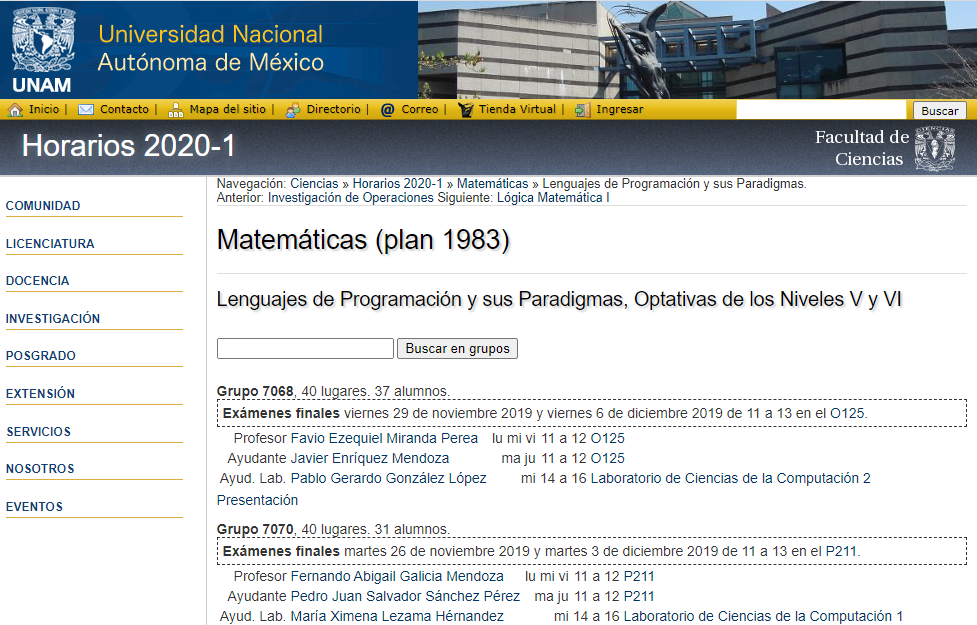
\includegraphics[width=\textwidth]{Fuente_de_info} %scale = 0.5
%\url{http://www.fciencias.unam.mx/docencia/horarios/20201/217/607} %%URL de la imagen
\caption[\textit{Página de horarios de la Facultad}]{\textit{Se muestra un ejemplo de una página de horarios de la Facultad. Se puede ver la información de los horarios de la materia ``Lenguajes de Programación y sus Paradigmas'', de la carrera de Matemáticas, plan 1983, del semestre 2020-1.}}\label{pagFC}
\end{figure}

La información que se puede extraer de las páginas mencionadas es: \textit{nombre de profesores, nombre de ayudantes, salón, horario, plan, carrera, año, número de semestre, materia, semestre de la materia, tipo de materia} e \textit{información de exámenes finales}.


\section{Estructura de las URL's}

Al iniciar la búsqueda de información notamos que las URL's de las páginas web de los horarios de la Facultad tienen una estructura similar. Ésto nos permitió poder realizar la búsqueda de la información de una manera automática y mucho más rápida. Observamos que la estructura que siguen las URL's mencionadas es la siguiente:

\begin{center}
\textit{\textbf{http://www.fciencias.unam.mx/docencia/horarios/a/b/c}}
\end{center}

Se tiene una raíz común para todas las páginas y al final se tienen tres números los cuales representan:

\begin{itemize}
\item[ ] \textit{\textbf{a}} = año y número de semestre

\item[ ] \textit{\textbf{b}} = clave del plan de estudios

\item[ ] \textit{\textbf{c}} = número de materia
\end{itemize}

Para este trabajo tomamos en cuenta sólo los planes de estudio vigentes hasta el semestre 2020-1. Es decir, tomamos todos los planes mostrados en la tabla \tablename{~\ref{PlanesEstudio}}, salvo el plan 1972 de Actuaría (el cual ya no está vigente). Dicha tabla muestra los planes de estudio de cada carrera con su clave correspondiente.

\begin{table}[h]
\centering
\begin{tabular}{|c|c|}
 \hline 
  \textbf{PLAN} & \textbf{CLAVE} \\ 
 \hline 
 \multicolumn{2}{|c|}{Actuaría} \\ 
 \hline 
 1972 & 214 \\ 
 \hline 
 2000 & 119 \\ 
 \hline 
 2006 & 1176 \\ 
 \hline 
 2015 & 2017 \\ 
 \hline 
 \multicolumn{2}{|c|}{Ciencias de la Computación} \\ 
 \hline 
 1994 & 218 \\ 
 \hline 
 2013 & 1556 \\ 
 \hline 
 \multicolumn{2}{|c|}{Matemáticas} \\ 
 \hline 
 1983 & 217 \\ 
 \hline 
 \multicolumn{2}{|c|}{Matemáticas Aplicadas} \\ 
 \hline 
 2017 & 2055 \\ 
 \hline 
 \end{tabular}
\caption[\textit{Planes de estudio por carrera con clave}]{\textit{Se muestran los planes de estudio por carrera con clave. Se sustituye \textbf{b} por la clave de cada plan de estudios, en la estructura de las URL's de las páginas de la Facultad.}}\label{PlanesEstudio}
\end{table}

Una vez identificada la estructura de las URL's pudimos realizar la búsqueda de información de manera automatizada. Originalmente decidimos que $c \in \{1,2,3, \ldots, 10 000\}$. Después hicimos una función que genera una matriz llamada \textit{mat\_posibles\_url}. La función sólo guarda las URL's que si existen.

La descripción de lo que contiene cada columna de la matriz \textit{mat\_posibles\_url} la podemos ver en la \tablename{~\ref{matPosiblesURL}}. Finalmente al obtener dicha matriz, observamos que el valor máximo que toma $c$ es 991, por lo que redujimos su conjunto de posibles valores y definimos $c \in \{1, \ldots, 1 000\}$.

\dfNmatrizChica %%Tabla con la información de la matriz chica

Decidimos buscar información en 25 semestres, del 2008-1 al 2020-1. Al multiplicar el número de semestres por los posibles valores de \textbf{c} obtuvimos $25 \times \textbf{c} = 25,000$. Este valor es una aproximación del número de posibles URL's con información de los horarios de la Facultad. Notemos que no estamos contando los planes de estudio, de ser así el número supera las $170,000$ posibles URL's.

Deseamos obtener información de cada una de esas páginas. Obtener dicha información ingresando a cada una de las páginas es muy tardado por lo que es necesario hacerlo de manera automatizada. Para extraer los datos de las páginas de la Facultad utilizamos una aplicación de \textit{Google Chrome} llamada \textit{SelectorGadget}. En la siguiente sección, explicaremos como obtuvimos los datos de las páginas de la Facultad con dicha aplicación.

\section{Extracción de datos con la aplicación SelectorGadget} \label{sec_ED_SelectorGadget}

La aplicación \textit{SelectorGadget} permite seleccionar la información deseada y arroja una sección del código CSS de una página web. Dicho código se introduce en \textit{R} para poder seleccionar y descargar la información deseada.

A continuación veremos los pasos que se deben de seguir para obtener el código CSS de la información seleccionada. Los colores y señalizaciones mencionados hacen referencia a la \figurename{~\ref{appSelectorGadget}}. %En dicha figura podemos ver un ejemplo del funcionamiento de la aplicación.

\begin{enumerate}
\item Presionar el ícono de la aplicación, el cual es una lupa (señalado por la flecha roja).

\item Seleccionar la información deseada (en color verde).

\item La aplicación automáticamente selecciona todas las entradas que coindiciden (en color amarillo).

\item En caso de que se haya seleccionado más información de la deseada entonces dar click sobre la información excedente (en color rojo).

\item  En el cuadro de texto, la aplicación arroja la sección del código CSS correspondiente a la información seleccionada. También muestra el número de entradas selecionadas (en óvalos rojos).
\end{enumerate}


\begin{figure}[H]
\centering
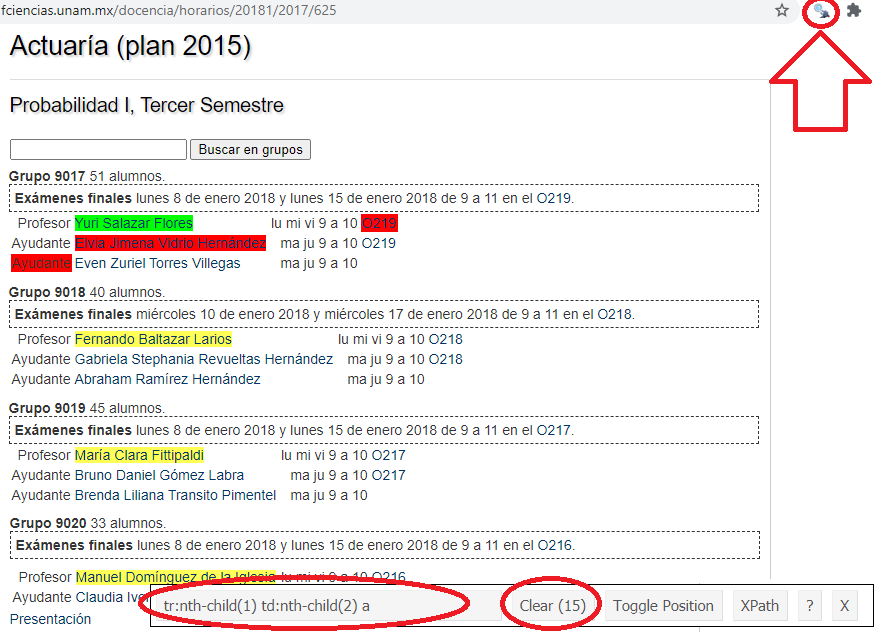
\includegraphics[width=\textwidth]{SelectorGadget} %scale = 0.65
%\url{http://www.fciencias.unam.mx/docencia/horarios/20181/2017/625} %%URL de la imagen
\caption[\textit{Uso de la aplicación SelectorGadget}]{\textit{En esta figura se muestra cómo se ve una página de horarios de la Facultad al usar la aplicación SelectorGadget mientras se selecciona la información que deseamos extraer.}}\label{appSelectorGadget}
\end{figure}

En el ejemplo mostrado en la \figurename{~\ref{appSelectorGadget}}, se seleccionaron 15 entradas correspondientes a los nombres de los profesores en una página con la información de la materia \textit{Probabilidad I}, en el plan 2015 de Actuaría. Los pasos a seguir son los mismos sin importar la información que se desea obtener, lo único que cambia es el código CSS que arroja la aplicación.

Sabiendo ésto, hicimos un ciclo en \textit{R} que recorre todas las posibles combinaciones de las URL's. Encontramos 3 principales tipos de grupos, los cuales describiremos en la siguiente sección.


\section{Tipos de grupos en las páginas web de la Facultad de Ciencias} \label{TiposDeGpos}

Cada uno de los 3 tipos de grupos encontrados contienen información similar. Hicimos la separación de acuerdo a sus diferencias. Cabe mencionar que en este trabajo consideramos como semestre actual al semestre $2020-1$. En todos los grupos se puede encontrar la información del nombre de profesor, nombre del o de los ayudantes, salón, horario y el número de alumnos inscritos en el grupo.

\begin{enumerate}
\item[a)] En el tipo \textbf{A} se tienen las páginas correspondientes al semestre actual. Este tipo de grupo tiene la información del número de lugares diponibles por salón, pero no contiene la información de los exámenes finales, porque se considera que el semestres aún está en curso y aún no termina. En la \figurename{~\ref{GpoA}} podemos ver un ejemplo de este tipo de grupo.

\begin{figure}[H]
\centering
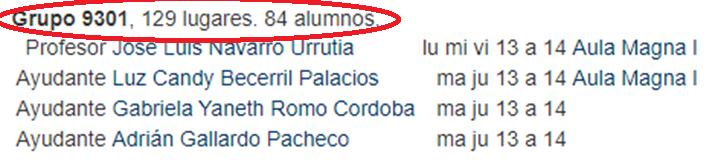
\includegraphics[width=\textwidth]{GrupoA} %scale = 0.8
%\url{http://www.fciencias.unam.mx/docencia/horarios/20201/2017/1707}
\caption[\textit{Tipo de grupo A}]{\textit{Se muestra un ejemplo de un grupo de tipo A. Corresponde al semestre actual (2020-1).}}\label{GpoA}
\end{figure}

\item[b)] En el tipo \textbf{B} se tienen las páginas correspondientes a semestres entre el $2018-2$ y el $2019-2$ (semestre anterior al actual). En este tipo de grupos se tiene información del número de lugares disponibles por salón y la información de los exámenes finales. Ésto porque son semestres que ya finalizaron. En la figura \figurename{~\ref{GpoB}} encontramos un ejemplo de este tipo de grupo.

\begin{figure}[H]
\centering
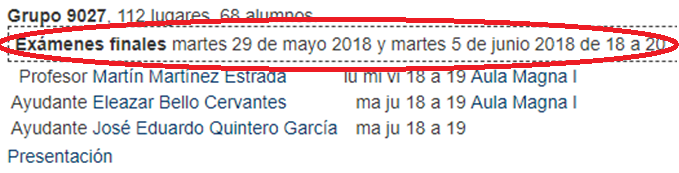
\includegraphics[width=\textwidth]{GrupoB} %scale = 0.8
%\url{http://www.fciencias.unam.mx/docencia/horarios/20182/217/625}
\caption[\textit{Tipo de grupo B}]{\textit{Se muestra un ejemplo de un grupo de tipo B. Corresponde a semestres ya finalizados, desde el 2018-2 hasta el 2019-2.}}\label{GpoB}
\end{figure}

\item[c)] En el tipo \textbf{C} se tienen las páginas correspondientes a semestres anteriores al $2018-1$, incluyéndolo. Este tipo de grupos tiene información de los exámenes finales, pero no contiene la información del número de lugares disponibles por salón. En la figura \figurename{~\ref{GpoC}} podemos ver un ejemplo.

\begin{figure}[H]
\centering
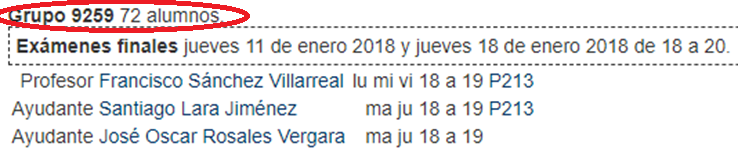
\includegraphics[width=\textwidth]{GrupoC} %scale = 0.8
%\url{http://www.fciencias.unam.mx/docencia/horarios/20181/1556/399}
\caption[\textit{Tipo de grupo C}]{\textit{Se muestra un ejemplo de un grupo de tipo C. Corresponde a semestres ya finalizados, anteriores al semestre 2018-1, incluyéndolo.}}\label{GpoC}
\end{figure}
\end{enumerate}


\section{Limpieza de base de datos} \label{sec_ED_LimpiezaDatos}

Se puede encontrar que, en general, cuando uno realiza la limpieza de datos se hace el 80\% del análisis de los datos. Es en ese momento en donde se encuentran los diferentes problemas que se pueden presentar. Se pueden encontrar posibles errores en los datos, información incompleta o valores poco comunes de acuerdo al comportamiento observado. Los problemas que encontramos al limpiar los datos se desglosan en las siguientes subsecciones.

\subsection{Problemas de falta de información}

Encontramos diferentes tipos de páginas que tenían grupos sin información e incluso páginas sin información alguna. Para guardar la información consideramos sólo los grupos que al menos tenían: nombre de profesor, número de alumnos inscritos y horario. A continuación se muestran varios ejemplos con los diferentes casos encontrados. %con falta de información.


\begin{itemize}
\item[-] En la figura \ref{pagEnBlanco} vemos un ejemplo de páginas en las cuales se tiene el nombre de la materia, pero no hay información de algún grupo: \url{http://www.fciencias.unam.mx/docencia/horarios/20081/1556/803}

\begin{figure}[H]
\centering
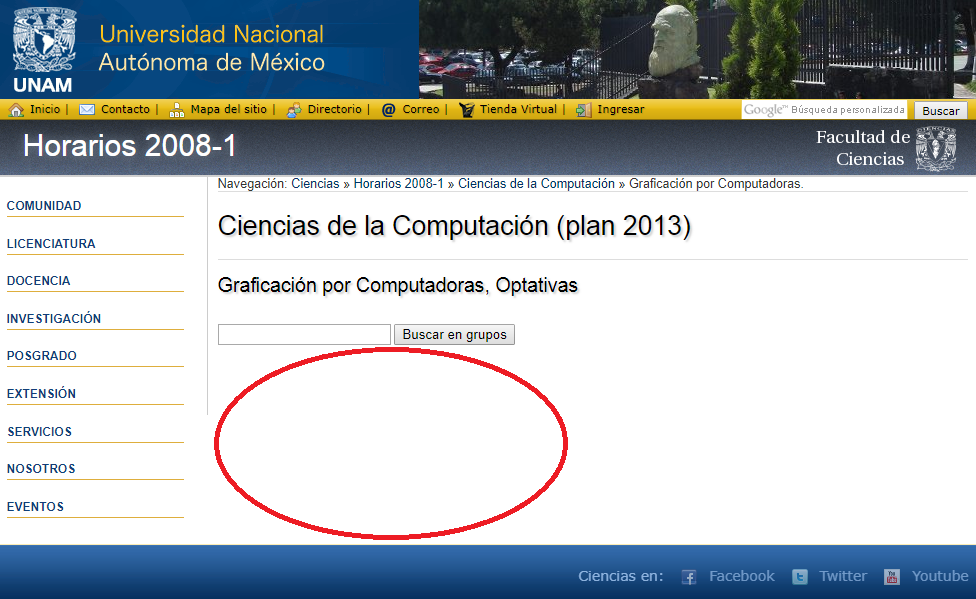
\includegraphics[scale = 0.45]{FaltaInfo_A} %width=\textwidth
\caption[\textit{Ejemplo de página web en blanco}]{\textit{Ejemplo de página web en blanco: En este tipo de páginas no encontramos información de los grupos para la materia.}}\label{pagEnBlanco}
\end{figure}

\item[-] En la figura \ref{GpoSinInfo} encontramos un ejemplo de páginas que no tienen información del salón: \url{http://www.fciencias.unam.mx/docencia/horarios/20081/119/4}

\begin{figure}[H]
\centering
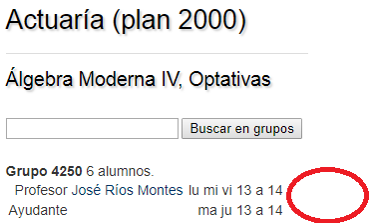
\includegraphics[scale = 0.45]{FaltaInfo_B} %width=\textwidth
\caption[\textit{Ejemplo de grupo sin información de salón}]{\textit{Ejemplo de grupo sin información de salón: En este tipo páginas no se muestra el salón en el que se imparte la clase.}}\label{GpoSinInfo}
\end{figure}

\item[-] En la figura \ref{GpoSinAlumnos} tenemos un ejemplo de páginas que tienen grupos sin información del número de alumnos inscritos en el grupo: \url{http://www.fciencias.unam.mx/docencia/horarios/20112/119/630}

\begin{figure}[H]
\centering
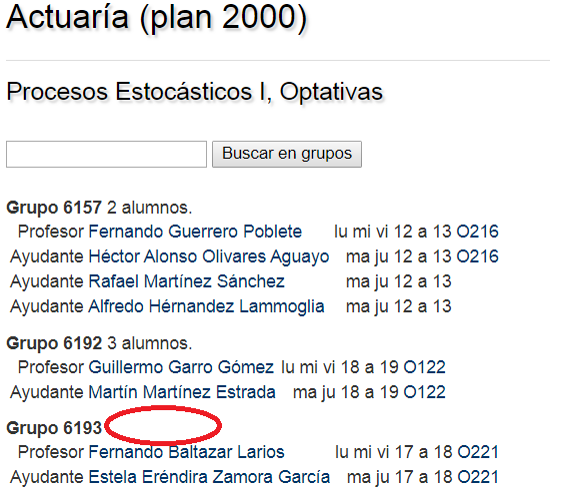
\includegraphics[scale = 0.6]{FaltaInfo_C} %width=\textwidth
\caption[\textit{Ejemplo de grupo sin información de alumnos}]{\textit{Ejemplo de grupo sin información de alumnos: En este tipo páginas encontramos grupos que no tienen el número de alumnos inscritos.}}\label{GpoSinAlumnos}
\end{figure}

\item[-] En la figura \ref{SoloHorario} vemos un ejemplo de páginas que tienen grupos sólo con el horario, sin nombre del profesor, salón, ayudante, número de alumnos, lugares disponibles: \url{http://www.fciencias.unam.mx/docencia/horarios/20091/119/841} %\url{http://www.fciencias.unam.mx/docencia/horarios/20091/119/244}

\begin{figure}[H]
\centering
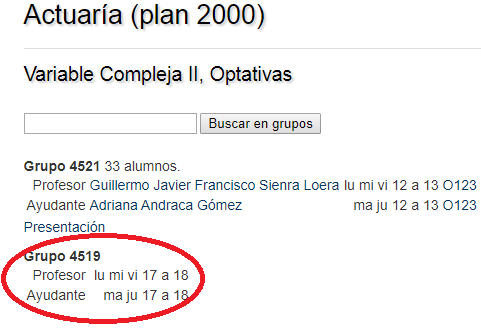
\includegraphics[scale = 0.8]{FaltaInfo_D} %width=\textwidth
\caption[\textit{Ejemplo de grupo sólo con horario}]{\textit{Ejemplo de grupo sólo con horario: En este tipo páginas existen grupos que no tienen información del profesor o salón ni del número de alumnos inscritos, sólo tienen la clave del grupo y el horario.}}\label{SoloHorario}
\end{figure}
\end{itemize} %%Subsección %%To include subfiles in to a subfiles use \input{name_of_file}
\subsection{Problemas de información repetida}

Dentro de los problemas de información repetida, encontramos diferentes casos. Para guardar la información juntamos aquellos grupos que provenían del mismo grupo. A continuación presentamos los casos que encontramos con el problema de tener información repetida.

\begin{itemize}
\item[-] En la \figurename{\ref{planRepetido}} mostramos un ejemplo en donde se tiene información de una materia correspondiente a un plan de estudios posterior al semestre en el que se está buscando la información: \url{http://www.fciencias.unam.mx/docencia/horarios/20082/1556/803} y tener la misma información con el plan de estudios correspondiente: \url{http://www.fciencias.unam.mx/docencia/horarios/20082/218/803}

El número del plan de estudios corresponde al año en que entró en vigencia el plan, por lo que no debería de existir un horario con un plan posterior al año del semestre. En la subfigura $(a)$ de la \figurename{\ref{planRepetido}} podemos ver una materia de la carrera de Ciencias de la Computación del semestre 2008-2, con el plan 2013, lo cual no es lógico. En la subfigura $(b)$ de la misma figura, vemos la infomración de la misma materia y del mismo grupo pero con el plan 1994.

\begin{figure}[H]
\centering
\subfigure[\textit{Plan de estudios posterior}]{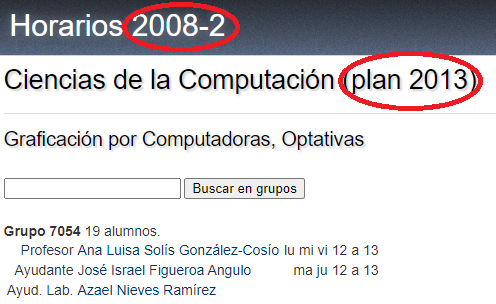
\includegraphics[width=10cm]{InfoRepetida_A_1}} %%Ping\"uino %%[angle=30]
	\subfigure[\textit{Plan de estudios correspondiente}]{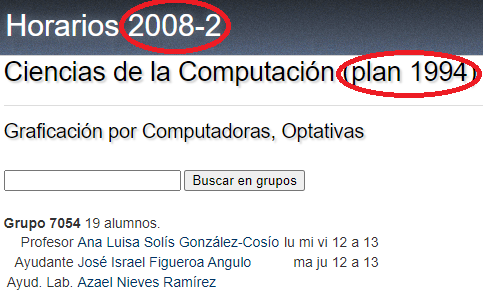
\includegraphics[width=10cm]{InfoRepetida_A_2}}
	\caption[\textit{Ejemplo de información repetida: Planes de estudio}]{\textit{Ejemplo de información repetida (Planes de estudio): No deberían de existir grupos con planes posteriores al año del semestre en el que se busca información.}}\label{planRepetido}
\end{figure}

\item[-] En la \figurename{\ref{MateriaNombresDistintos}} vemos un ejemplo en donde se tiene una misma materia con nombres distintos para las diferentes carreras: \url{http://www.fciencias.unam.mx/docencia/horarios/20201/217/1712} para Matemáicas, plan 1983 y \url{http://www.fciencias.unam.mx/docencia/horarios/20201/2017/1739} para Actuaría, plan 2015. Notamos que la información en ambas páginas es la misma, sólo cambian las claves de los grupos.

\begin{figure}[H]
	\centering
	\subfigure[\textit{Matemáticas: 1983}]{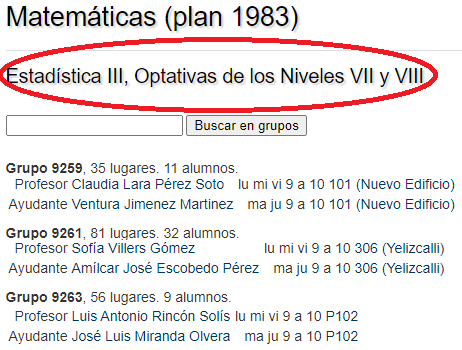
\includegraphics[width=10cm]{InfoRepetida_B_1}} %%Ping\"uino %%[angle=30]
	\subfigure[\textit{Actuaría: 2015}]{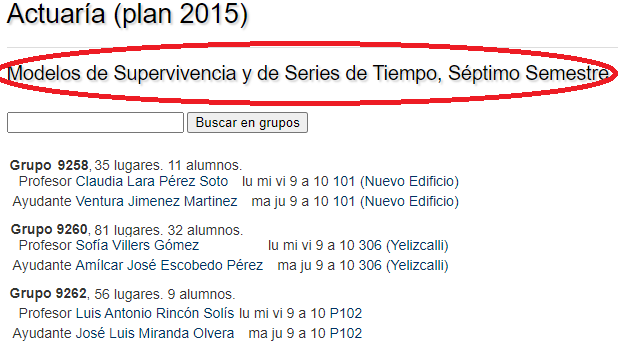
\includegraphics[width=10cm]{InfoRepetida_B_2}}
	\caption[\textit{Ejemplo de información repetida: Materia con nombres distintos}]{\textit{Ejemplo de información repetida: Materia con nombres distintos: En estos casos se tienen materias que tienen nombres diferentes de acuerdo a la carrera o plan de estudios.}}\label{MateriaNombresDistintos}
\end{figure}

\item[-] En la \figurename{\ref{UnProfMuchasMaterias}} tenemos un ejemplo de profesores que imparten dos o más clases distintas en el mismo horario y diferente salón: \url{http://www.fciencias.unam.mx/docencia/horarios/20111/2017/162} para Ecuaciones Diferenciales I y \url{http://www.fciencias.unam.mx/docencia/horarios/20111/2017/91} para Cálculo Diferencial e Integral I.
  
Las materias mencionadas son diferentes, pero las clases comienzan a la misma hora, Ecuaciones de 18-19hrs y Cálculo de 18-20hrs, dado que se tiene la misma ayudante pudiera ser que se intercambien las horas, pero no se puede asignar más de una clase a la misma hora al mismo profesor.

%EJEMPLO CON PROFESOR: Bartolo Guzmán Guevara
%Ecuaciones Diferenciales Parciales II
%\url{http://www.fciencias.unam.mx/docencia/horarios/20131/217/183}
%\url{http://www.fciencias.unam.mx/docencia/horarios/20131/119/183}
%\url{http://www.fciencias.unam.mx/docencia/horarios/20131/2055/183}
%Matemáticas Avanzadas de la Física
%\url{http://www.fciencias.unam.mx/docencia/horarios/20131/217/610}
%Funciones Especiales y Transformadas Integrales
%\url{http://www.fciencias.unam.mx/docencia/horarios/20131/218/217}
%\url{http://www.fciencias.unam.mx/docencia/horarios/20131/119/217}

%EJEMPLO CON PROFESORA: Tania Eréndira Rivera Torres. Introducción Matemática a la Mecánica Celeste y Álgebra Lineal I
%http://www.fciencias.unam.mx/docencia/horarios/20082/119/5
%http://www.fciencias.unam.mx/docencia/horarios/20082/119/356
%http://www.fciencias.unam.mx/docencia/horarios/20082/1176/5
%http://www.fciencias.unam.mx/docencia/horarios/20082/2017/5
%http://www.fciencias.unam.mx/docencia/horarios/20082/218/5
%http://www.fciencias.unam.mx/docencia/horarios/20082/1556/5
%http://www.fciencias.unam.mx/docencia/horarios/20082/217/5
%http://www.fciencias.unam.mx/docencia/horarios/20082/217/356
%http://www.fciencias.unam.mx/docencia/horarios/20082/2055/5 

%EJEMPLO CON PROFESOR: Hugo Alberto Rincón Mejía. Álgebra Moderna II y Álgebra Moderna III
%http://www.fciencias.unam.mx/docencia/horarios/20192/119/2
%http://www.fciencias.unam.mx/docencia/horarios/20081/119/3
%http://www.fciencias.unam.mx/docencia/horarios/20192/218/2
%http://www.fciencias.unam.mx/docencia/horarios/20192/1556/2
%http://www.fciencias.unam.mx/docencia/horarios/20192/217/2

%EJEMPLO CON PROFESOR: Roberto Pichardo Mendoza. Seminario de Apoyo a la Titulación en Matemáticas A y Geometría Analítica II
%http://www.fciencias.unam.mx/docencia/horarios/20192/119/245
%http://www.fciencias.unam.mx/docencia/horarios/20192/1176/245
%http://www.fciencias.unam.mx/docencia/horarios/20192/2017/245
%http://www.fciencias.unam.mx/docencia/horarios/20192/218/245
%http://www.fciencias.unam.mx/docencia/horarios/20192/217/245
%http://www.fciencias.unam.mx/docencia/horarios/20192/217/959
%http://www.fciencias.unam.mx/docencia/horarios/20192/2055/245

%EJEMPLO CON PROFESOR: Roberto Pichardo Mendoza. Seminario de Topología A y Seminario de Apoyo a la Titulación en Matemáticas A
%http://www.fciencias.unam.mx/docencia/horarios/20191/119/977
%http://www.fciencias.unam.mx/docencia/horarios/20191/217/959
%http://www.fciencias.unam.mx/docencia/horarios/20191/217/977

%EJEMPLO CON PROFESOR: Sergio Iván López Ortega. Probabilidad II y Procesos Estocásticos II
%http://www.fciencias.unam.mx/docencia/horarios/20112/119/626
%http://www.fciencias.unam.mx/docencia/horarios/20112/119/631
%http://www.fciencias.unam.mx/docencia/horarios/20112/1176/626
%http://www.fciencias.unam.mx/docencia/horarios/20112/1176/631
%http://www.fciencias.unam.mx/docencia/horarios/20112/2017/626
%http://www.fciencias.unam.mx/docencia/horarios/20112/2017/631
%http://www.fciencias.unam.mx/docencia/horarios/20112/218/626
%http://www.fciencias.unam.mx/docencia/horarios/20112/1556/626
%http://www.fciencias.unam.mx/docencia/horarios/20112/217/626
%http://www.fciencias.unam.mx/docencia/horarios/20112/217/631
%http://www.fciencias.unam.mx/docencia/horarios/20112/2055/626
%http://www.fciencias.unam.mx/docencia/horarios/20112/2055/631

%EJEMPLO CON PROFESORA: Ana Patricia Kuri González. Seminario sobre Enseñanza de las Matemáticas II y Seminario sobre Enseñanza de las Matemáticas I
%http://www.fciencias.unam.mx/docencia/horarios/20172/119/751
%http://www.fciencias.unam.mx/docencia/horarios/20172/119/754
%http://www.fciencias.unam.mx/docencia/horarios/20172/218/751
%http://www.fciencias.unam.mx/docencia/horarios/20172/218/754
%http://www.fciencias.unam.mx/docencia/horarios/20172/217/751
%http://www.fciencias.unam.mx/docencia/horarios/20172/217/754

%EJEMPLO CON PROFESORA: Tania Eréndira Rivera Torres. Introducción Matemática a la Mecánica Celeste y Álgebra Lineal I
%http://www.fciencias.unam.mx/docencia/horarios/20082/119/5
%http://www.fciencias.unam.mx/docencia/horarios/20082/119/356
%http://www.fciencias.unam.mx/docencia/horarios/20082/1176/5
%http://www.fciencias.unam.mx/docencia/horarios/20082/2017/5
%http://www.fciencias.unam.mx/docencia/horarios/20082/218/5
%http://www.fciencias.unam.mx/docencia/horarios/20082/1556/5
%http://www.fciencias.unam.mx/docencia/horarios/20082/217/5
%http://www.fciencias.unam.mx/docencia/horarios/20082/217/356
%http://www.fciencias.unam.mx/docencia/horarios/20082/2055/5

%EJEMPLO CON PROFESOR: Juan Rivera Alcántara. Teoría del Riesgo y Valuación de Opciones
%http://www.fciencias.unam.mx/docencia/horarios/20082/119/1067
%http://www.fciencias.unam.mx/docencia/horarios/20082/119/1807
%http://www.fciencias.unam.mx/docencia/horarios/20082/1176/1067
%http://www.fciencias.unam.mx/docencia/horarios/20082/1176/1807
%http://www.fciencias.unam.mx/docencia/horarios/20082/2017/1807

%EJEMPLO CON PROFESOR: Javier Valdez Quijada. Teoría de los Números I y Teoría de los Números II
%http://www.fciencias.unam.mx/docencia/horarios/20172/119/764
%http://www.fciencias.unam.mx/docencia/horarios/20172/119/777
%http://www.fciencias.unam.mx/docencia/horarios/20172/218/764
%http://www.fciencias.unam.mx/docencia/horarios/20172/218/777
%http://www.fciencias.unam.mx/docencia/horarios/20172/1556/764
%http://www.fciencias.unam.mx/docencia/horarios/20172/1556/777
%http://www.fciencias.unam.mx/docencia/horarios/20172/217/764
%http://www.fciencias.unam.mx/docencia/horarios/20172/217/777



%EJEMPLO CON PROFESOR: 
%EJEMPLO CON PROFESORA: 


\begin{figure}[H]
	\centering
	\subfigure[\textit{Ecuaciones Diferenciales I}]{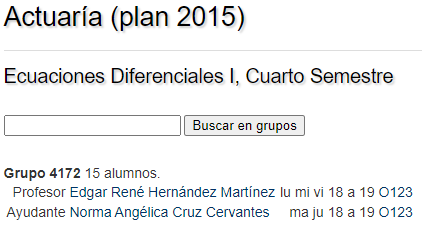
\includegraphics[width=10cm]{Ej_gpo_repetido_1}} %%Ping\"uino %%[angle=30]
	\subfigure[\textit{Cálculo Diferencial e Integral I}]{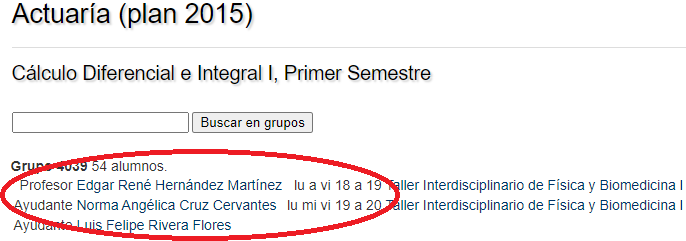
\includegraphics[width=15cm]{Ej_gpo_repetido_2}}
	\caption[\textit{Ejemplo de información repetida: Mismo profesor, materias distintas}]{\textit{Ejemplo de información repetida (mismo profesor, materias distintas): En este caso se tiene más de una clase impartida por el mismo profesor a la misma hora en diferente salón lo cual no debería de ocurrir.}}\label{UnProfMuchasMaterias}
\end{figure}	

\end{itemize}
 %%Subsección
\subsection{Otros problemas al extraer información}

En algunos de los problemas que surgieron, encontramos detalles particulares que tuvimos que resolver caso por caso. Ésto para poder guardar la información de manera adecuada. A continuación se presentan los diferentes casos encontrados:

  \begin{itemize}
\item[-] Dentro de la obtención de datos del número de alumnos, no se lee la información cuando se tiene \textit{Un alumno}, ya que no se reconoce el texto \textit{Un} como el número $1$. En la \figurename{~\ref{UnAlumno}} vemos un ejemplo de este caso.

\begin{figure}[H]
\centering
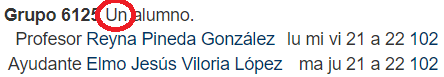
\includegraphics[scale = 0.8]{Ej_un_alumno} %width=\textwidth
%\url{http://www.fciencias.unam.mx/docencia/horarios/20081/119/1809}
\caption[\textit{Ejemplo de grupo con un alumno}]{\textit{Ejemplo de grupo con un alumno: En este caso se tiene el texto ``Un'' y no un número ``1''.}}\label{UnAlumno}
\end{figure}

Para resolver este problema se identificó la variable tipo \textit{string} igual a \textit{Un} para convertir la información y así poder utilizar los datos obtenidos.

\item[-] El algoritmo supone que todas las clases duran una hora y no se consideran las medias horas: \url{http://www.fciencias.unam.mx/docencia/horarios/20172/1556/820}. En la \figurename{~\ref{MediasHoras}} mostramos un ejemplo en donde se considera que esa materia inicia a las 18hrs.

\begin{figure}[H]
\centering
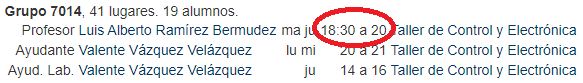
\includegraphics[scale = 0.9]{Ej_gpo_medias_hrs} %width=\textwidth
%\url{http://www.fciencias.unam.mx/docencia/horarios/20172/1556/820}
\caption[\textit{Ejemplo de grupo con medias horas}]{\textit{Ejemplo de grupo con medias horas: Se considera que las materias inician en horas enteras y no a las medias horas.}}\label{MediasHoras}
\end{figure}

\item[-] Se tienen materias con múltiples horarios: \url{http://www.fciencias.unam.mx/docencia/horarios/20181/2055/1323}. En estos casos sólo se registran los horarios y salones en los que los profesores imparten su clase, no se toman en cuenta las clases impartidas por los ayudantes.

En la \figurename{~\ref{horariosMultiples}} tenemos un ejemplo de este caso en donde el profesor imparte su clase los lunes, miércoles y viernes de 13-14hrs en el salón O215, hay una ayudantía los martes y jueves de 13-14hrs en el salón O215 y otra ayudantía los martes de 11-13hrs en el salón 304 (Yelizcalli). Se considera que esta materia inicia a las 13hrs y se imparte en el salón O215.

\begin{figure}[H]
\centering
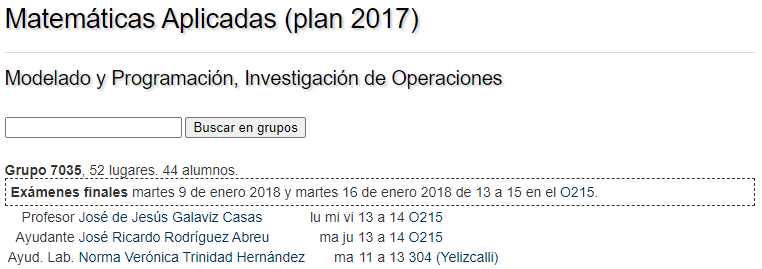
\includegraphics[scale = 0.8]{Ej_gpo_horarios_multiples} %width=\textwidth
\caption[\textit{Ejemplo de grupo con horarios múltiples}]{\textit{Ejemplo de grupo con horarios múltiples: En estos grupos sólo se toman en cuenta los horarios y salones en los que los profesores imparten clase.}}\label{horariosMultiples}
\end{figure}

\item[-] Las materias de inglés no se imparten todos los días de la semana, en algunos casos se imparten clases en línea: \url{http://www.fciencias.unam.mx/docencia/horarios/20202/2017/1135}. Se registran únicamente los horarios de los días en que se imparten las clases presenciales. En la \figurename{~\ref{casoIngles}} mostramos un ejemplo de este caso.

\begin{figure}[H]
\centering
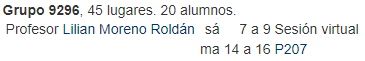
\includegraphics[scale = 1]{Ej_gpo_ingles} %width=\textwidth
\caption[\textit{Ejemplo de grupo de inglés}]{\textit{Ejemplo de grupo de inglés: Las clases no se imparten todos los días. Hay sesiones virtuales. Sólo se toma en cuenta el horario de las clases presenciales.}}\label{casoIngles}
\end{figure}

\item[-] Se tienen grupos que no tienen la misma estructura que los tipos de grupos \textbf{A}, \textbf{B} y \textbf{C} definidos en la Sección \ref{TiposDeGpos}: \url{http://www.fciencias.unam.mx/docencia/horarios/20201/2017/872}, debido a ello el código CSS utilizado no sirve para obtener toda la información que se puede obtener del grupo. En la \figurename{~\ref{GpoEstructuraDiferente}} tenemos un ejemplo de este caso en donde no se lee adecuadamente el número de alumnos inscritos en el grupo.

\begin{figure}[H]
\centering
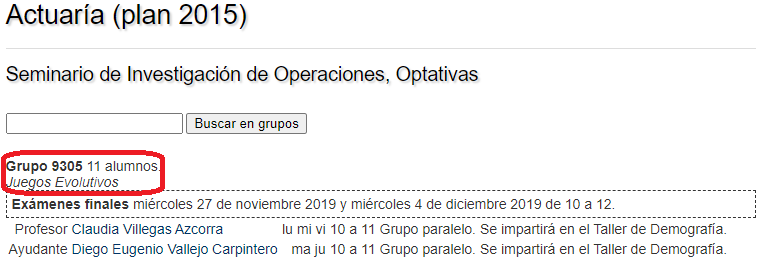
\includegraphics[scale = 0.8]{Ej_gpo_con_estructura_diferente} %width=\textwidth
\caption[\textit{Ejemplo de grupo con estructura diferente}]{\textit{Ejemplo de grupo con estructura diferente: En estos casos no se extrae adecuadamente la información de los grupos porque el código CSS utilizado no corresponde a este tipo de grupos.}}\label{GpoEstructuraDiferente}
\end{figure}

\end{itemize} %%Subsección

\section{Matrices de datos}

Una vez que se realizó el proceso de limpieza de los datos obtenidos, éstos se guardaron, por semestre, en matrices llamadas \textit{m\_grande}. Los nombres de sus columnas con su respectiva explicación y posibles valores, se muestran en la siguiente tabla. Cabe aclarar que la abreviatura \textit{CdC} denota \textit{Ciencias de la Computación} y \textit{MatAp} denota \textit{Matemáticas Aplicadas}.

\dfNmatrizGrande %%Tabla con la información de la matriz grande

La columna \textit{Cambios}, va a guardar todos los cambios que ha tenido cada grupo. El significado de los números que pueden aparecer en esa columna se explican a continuación:

\begin{enumerate}
\item[(1)] Grupos que se revisaron individualmente por tener detalles particulares.

\item[(2)] Se anotaron los días en los que se imparte la materia, en la columna \textit{Horario}, por ejemplo cuando había conflicto debido a que el profesor impartía más de una materia a la misma hora, al revisar el caso se encontró que los días en los que se impartía la clase era distinto.

\item[(3)] Se eliminaron los grupos repetidos, al juntar la información en un mismo grupo.

\item[(4)] Páginas que no tienen información del salón.

\item[(5)] Actualización del número de materia por cambio de nombre o agrupamiento de materias.
\end{enumerate}
 %%2

\chapter{Análisis estadístico}

%Teniendo los datos guardados y limpios, proseguimos con la siguiente etapa del proyecto, se realizó un análisis estadístico de los datos. Para ello se observaron los grupos de datos en los que se dividió la información, se eligió el método Holt-Winters aditivo el cual funciona para series de tiempo con componentes de tendencia aproximadamente lineal y de estacionalidad.

%Teniendo los datos guardados y limpios, se realizó un análisis estadístico de los datos, las herramientas elegidas para dicho análisis fueron las series de tiempo y el método Holt-Winters aditivo el cual funciona para series de tiempo con componentes de tendencia aproximadamente lineal y de estacionalidad.

Debido a la naturaleza de los datos, las herramientas elegidas para realizar un análisis estadístico de los datos fueron las series de tiempo. A continuación se describe su definición y aplicación para explicar el motivo de la elección de dichas herramientas estadísticas.

Definimos a una serie de tiempo como una secuencia de observaciones $X_{t}$ ordenadas cronológicamente. Los datos al tiempo presente dependen de las observaciones anteriores, es decir existe una depencia de $X_{t}$ con $\{X_{t-1}, X_{t-2}, X_{t-3}, \ldots, X_{2}, X_{1}, X_{0}, \ldots\}$.

Denotamos a una serie de tiempo como:
  \begin{equation}
X_{t} = m_{t} + s_{t} + y_{t},
\end{equation}
%Se dice que una serie de tiempo es estacionaria si a lo largo del tiempo su media y su varianza con constantes y es no estacionaria si su tendencia y variabilidad cambian en el tiempo. Sus componentes son:
donde las componentes de la serie de tiempo $m_{t}, s_{t}, y_{t},$ tienen las siguientes propiedades:

\begin{itemize}
\item[-] Tendencia $(m_{t})$: Se le llama tendencia al cambio, a largo plazo, del promedio de los datos. El cambio puede ser creciente o decreciente.

\item[-] Estacionalidad $(s_{t})$: Se llama variación estacional a las fluctuaciones periódicas que tiene una serie de tiempo. La longitud de cada periodo es constante y por lo general menor o igual a un año, por ejemplo semanal, mensual o semestral.

\item[-] Aleatoriedad $(y_{t})$: También llamada componente irregular, son series de residuales que pueden o no ser aleatorios.
\end{itemize}

Chatfield y Xing, en su libro \textit{The Analysis of Time Series An Introduction with R} [\ref{ChatfieldXing}], nos indican que existen 2 tipos de variación estacional:
  
  \begin{itemize}
\item[-] Aditiva: Se dice que la estacionalidad es aditiva cuando la longitud de cada periodo es constante año con año.

\item[-] Multiplicativa: Se dice que la estacionalidad es multiplicativa cuando la longitud de cada periodo es directamente proporcional a la media de los datos de la serie de tiempo.
\end{itemize}

Con estos tipos de variaciones se forman 3 modelos de estacionalidad:
  
  \begin{enumerate}
\item Aditivo: En este modelo se tiene variación estacional aditiva. Se utiliza cuando la varianza o la desviación estándar de la serie de tiempo se mantienen constantes a lo largo del tiempo. El modelo aditivo se denota como:
\begin{equation}
X_{t} = m_{t} + s_{t} + y_{t}.
\end{equation}

\item Multiplicativo: En este modelo se tiene variación estacional multiplicativa. Se utiliza cuando la varianza o la desviación estándar de los datos cambian a través del tiempo. Su variabilidad puede ser mayor o menor conforme pasa el tiempo. El modelo multiplicativo se denota como:
\begin{equation}
X_{t} = m_{t}s_{t}y_{t}.
\end{equation}

\item Mixto: Este modelo se utiliza cuando se tiene variación estacional multiplicativa pero la variabilidad de la componente irregular se mantiene constante a lo largo del tiempo. El modelo mixto se denota como:
\begin{equation}
X_{t} = m_{t}s_{t} + y_{t}.
\end{equation}
\end{enumerate}

Los objetivos principales al hacer el análisis de una serie de tiempo son:
  
  \begin{itemize}
\item[-] Describir: Leer datos en una tabla es mucho más tardado y en algunas ocasiones más complicado que observar una gráfica de los datos que se tienen. Las gráficas ayudan a ver de una manera más inmediata el comportamiento que tienen los datos y es posible observar si la serie de tiempo tiene alguna tendencia o estacionalidad. También se puede ver la posible falta de información o valores atípicos.

\item[-] Predecir: Teniendo una serie de tiempo se desea conocer qué va a pasar en el futuro. Es conveniente tener varios periodos de información para que la predicción sea lo más acertada posible.
\end{itemize}

Las áreas en las que se pueden aplicar las series de tiempo son por ejemplo en economía, demografía, finanzas, medio ambiente, ingeniería o medicina. En estas áreas, algunos ejemplos de su aplicación son: precios de acciones diarios, niveles de producción en la agricultura mensuales, medición del sonido por segundos, barriles de petróleo producidos al año, electrocardiogramas, medición de terremotos, tasa de mortalidad, tasa de natalidad, entre otros.


\section{Análisis estadístico básico}

En esta sección haremos un análisis básico de los datos correspondientes a las carreras del Departamento de Matemáticas. Para dicho análisis utilizaremos series de tiempo. Las técnicas de suavizamiento de series de tiempo son útiles para mostrar patrones subyacentes en los datos de las series de tiempo. El método que vamos a utilizar para mostrar dichos patrones de los datos es el método Holt-Winters aditivo.

%El método Holt-Winters aditivo se utiliza para describir y predecir valores con series de tiempo que tienen componentes de tendencia aproximadamente lineal y de estacionalidad.

Éste método se utiliza para describir y predecir valores de series de tiempo que tienen componentes de tendencia y de estacionalidad. Existen pruebas, que hemos aplicado a los datos, para comprobar que cumplen con los supuestos del método. En particular, estas pruebas se muestran a lo largo de esta sección.

Para analizar los datos, en esta sección presentamos varias gráficas. Específicamente, presentamos algunas gráficas de series de tiempo y otras de sus valores acumulados. Con ellas observaremos el comportamiento de los datos, veremos si tienen alguna tendencia o variación estacional.

En la \figurename{~\ref{TotalAlumBarras}} se muestra la gráfica de barras con el número total de alumnos que toman clases por semestre. A simple vista notamos que tiene una tendencia creciente y una estacionalidad semestral. Podemos ver también que, en general, el número de alumnos de los semestres impares es mayor al de su siguiente semestre par. Este fenómeno los vimos en la \figurename{~\ref{ParImparProbaI}} al hacer el análisis correspondiente a los datos de la materia \textit{Probabilidad I}.

\begin{figure}[H]
\centering
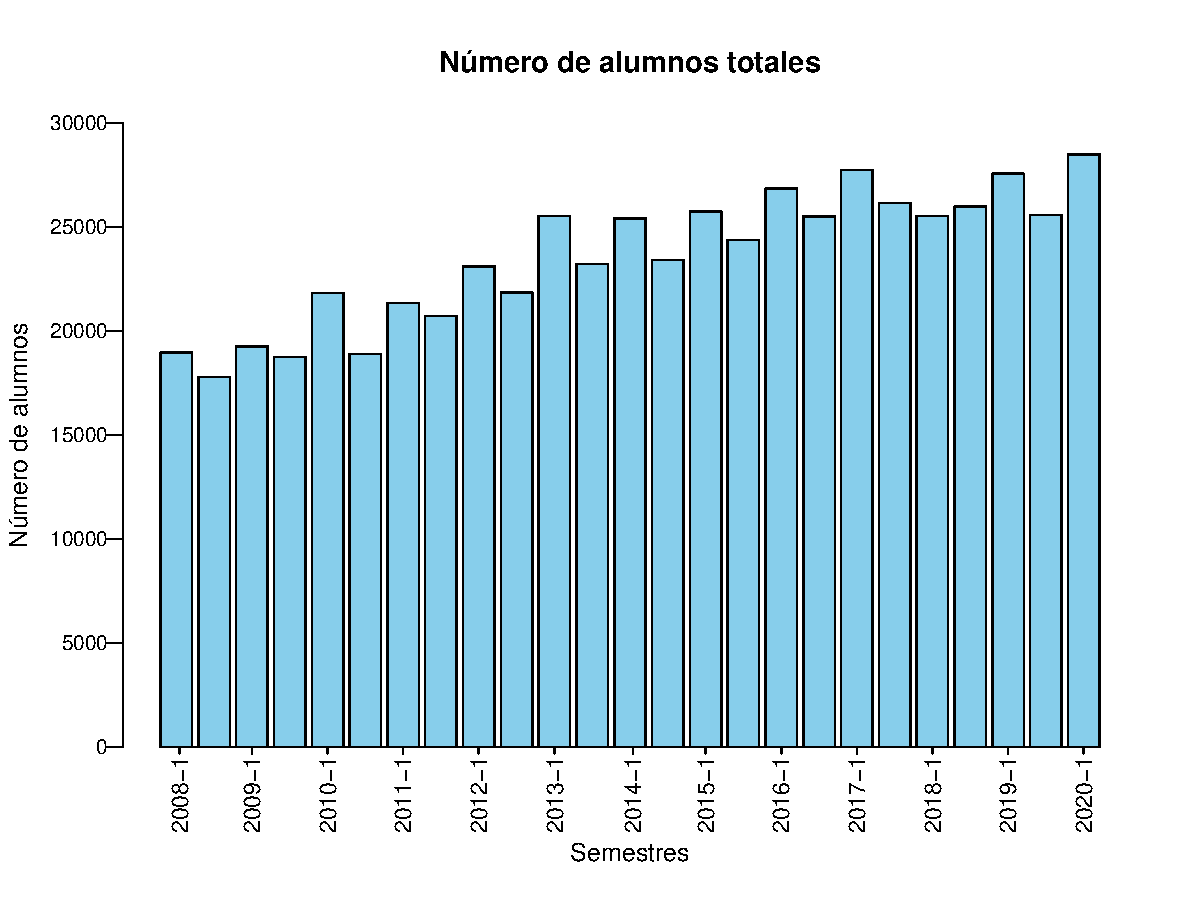
\includegraphics[scale = 0.8]{num_alum_total_x_sem_barplot} %width=\textwidth
\caption[\textit{Número total de alumnos por semestre}]{\textit{Número total de alumnos por semestre: En esta figura se muestra la gráfica de barras del número total de alumnos inscritos por cada semestre. Se observa que año con año el número aumenta. En general, el número de alumnos de los semestres impares es mayor que el de su respectivo semestre par.}}\label{TotalAlumBarras}
\end{figure}

En la \figurename{~\ref{prom_alum_x_sem_ts}} se muestra la gráfica de la media del número de alumnos que toman clases por semestre de todas las materias. Observamos que los valores tienen una tendencia creciente, ésto nos indica que cada semestre, en promedio, el número de alumnos incrementa en la Facultad.

\begin{figure}[H]
\centering
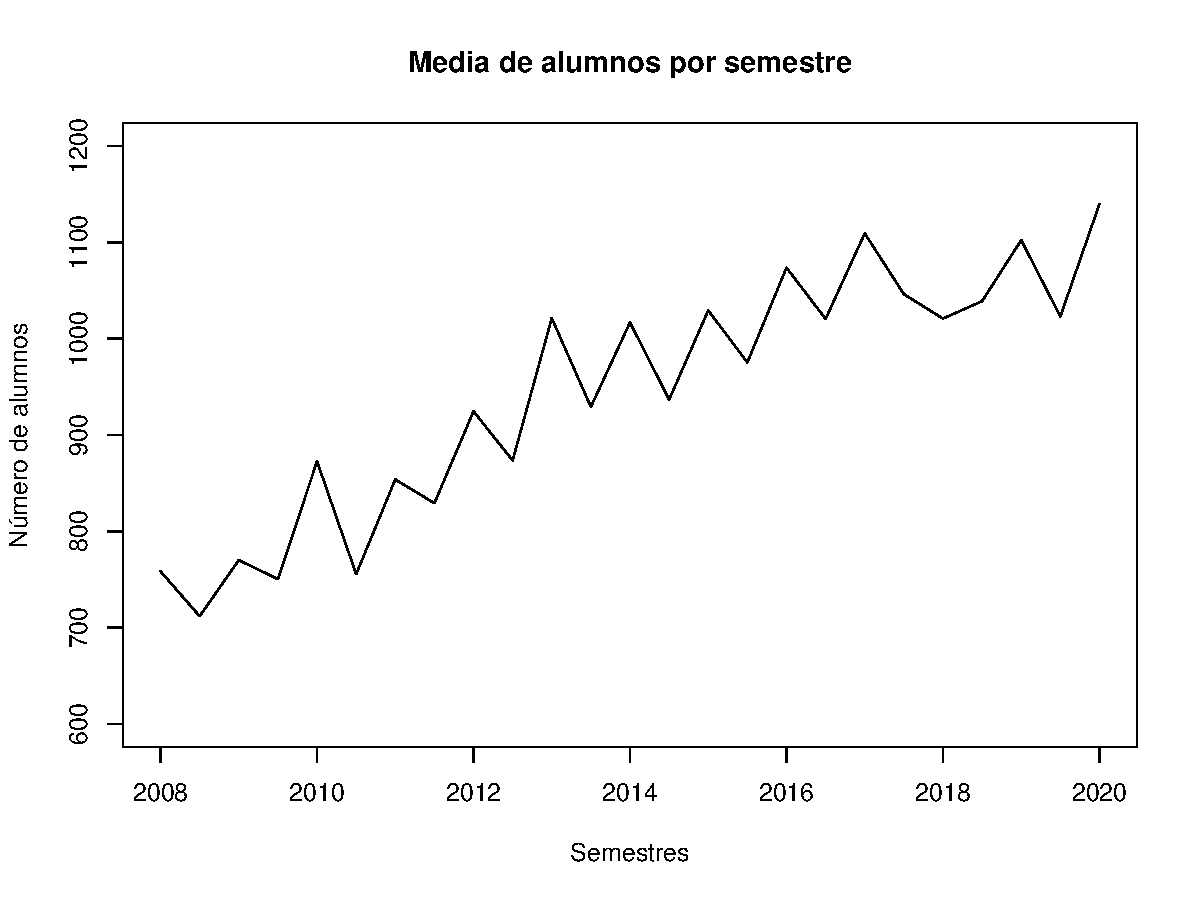
\includegraphics[scale = 0.6]{prom_alum_total_x_sem_ts.pdf} %width=\textwidth
\caption[\textit{Media de alumnos por semestre}]{\textit{Media de alumnos por semestre: Se observa una tendencia creciente en la media de alumnos por semestre. La información corresponde a los semestres del 2008-1 al 2020-1.}}\label{prom_alum_x_sem_ts}
\end{figure}

En la \figurename{~\ref{sd_alum_x_gpo_x_sem_ts}} se muestra la gráfica de la desviación estándar del número de alumnos por grupo y por semestre de todas las materias. Observamos que los valores se mantienen constantes a lo largo del tiempo, en un rango de entre 24 y 29 alumnos.

\begin{figure}[H]
\centering
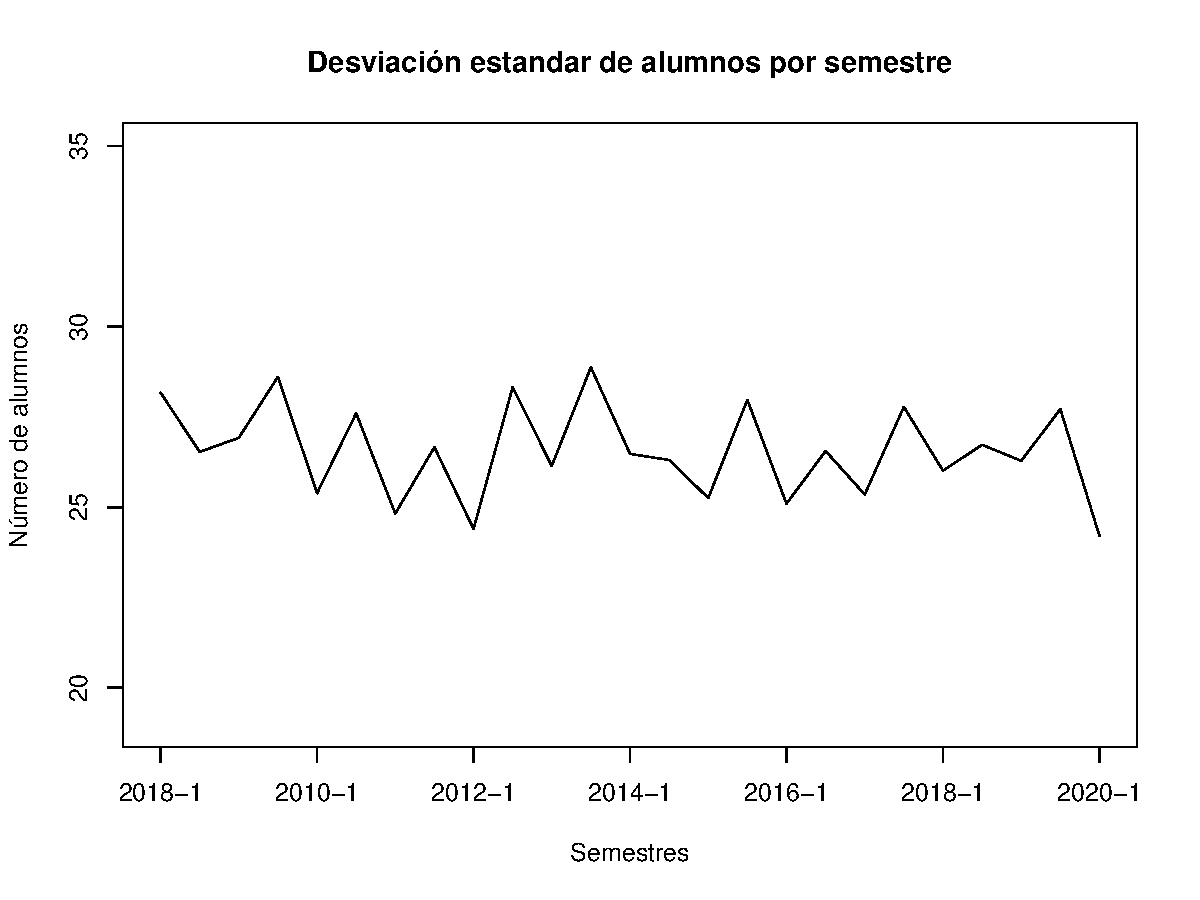
\includegraphics[scale = 0.6]{sd_alum_x_gpo_x_sem_ts.pdf} %width=\textwidth
\caption[\textit{Desviación estándar del número de alumnos por semestre}]{\textit{Desviación estándar del número de alumnos por semestre: Se muestra el comportamiento de los datos el cual es constante a lo largo del tiempo.}}\label{sd_alum_x_gpo_x_sem_ts}
\end{figure}

En la \figurename{~\ref{img_en_ing_2}} se observan 4 diferentes gráficas, en la primera, de arriba hacia abajo, se observan los datos reales del número total de alumnos para cada semestre. En la segunda se muestra la tendecia de los datos, la cual notamos que es creciente. En la tercera vemos la componente estacional que nos indica que los datos tienen una estacionalidad semestral. En la cuarta se ve la componente aleatoria de los datos la cual ya no tiene estacionalidad ni tendencia.

\begin{figure}[H]
\centering
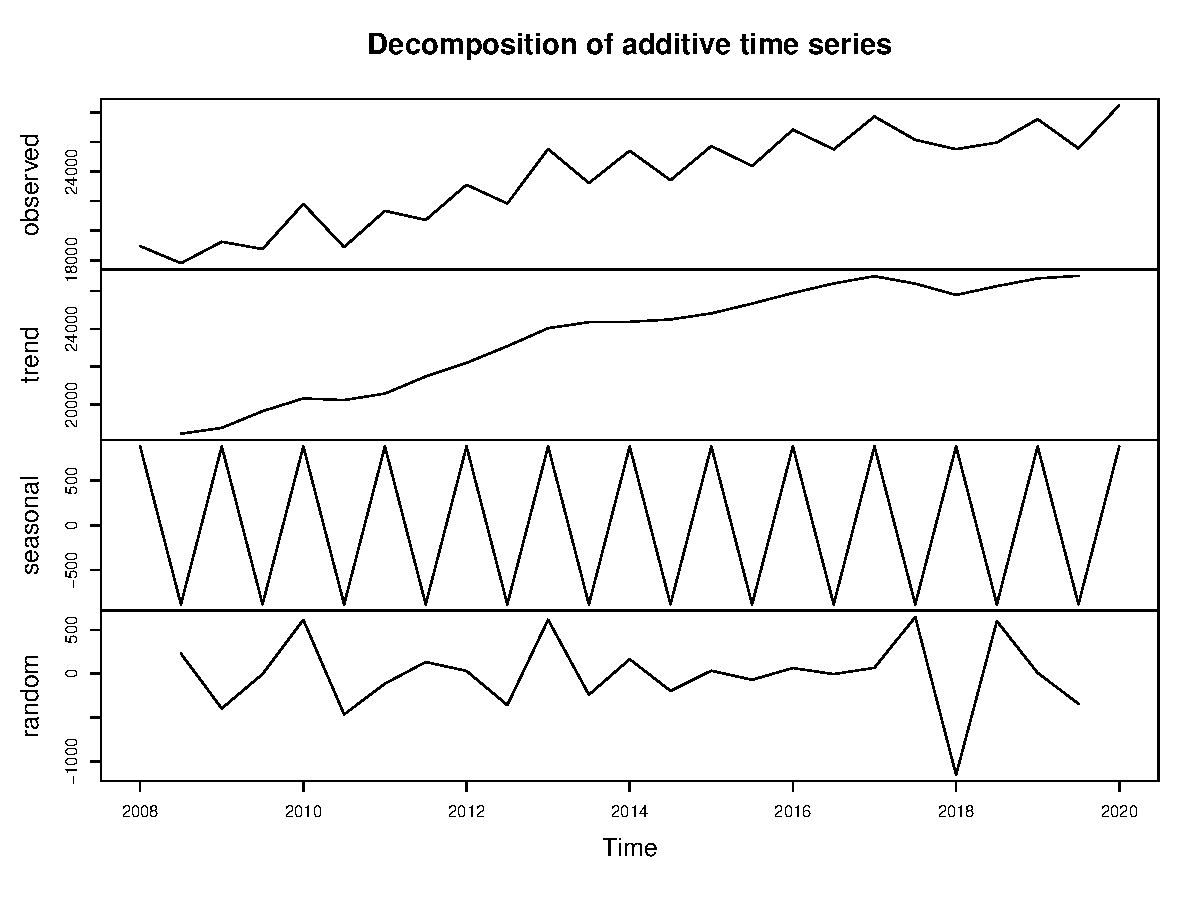
\includegraphics[width=\textwidth]{descomposicion_ts_total_alumnos.pdf} %scale = 0.8
\caption[\textit{Descomposición por el método aditivo de Holt-Winters}]{\textit{Descomposición por el método aditivo de Holt-Winters: Los datos considerados en esta descomposición es el número total de alumnos por semestre.}}\label{img_en_ing_2}
\end{figure}

Viendo la \figurename{~\ref{img_en_ing_2}} notamos que los datos tienen estacionalidad semestral y una tendencia creciente, por lo tanto confirmamos que se puede utilizar el método Holt-Winters ya que se cumplen los supuestos que se requieren. Para verificar que el modelo de estacionalidad adecuado es el aditivo, vemos la \figurename{~\ref{sd_alum_x_gpo_x_sem_ts}} y notamos que la desviación estándar permanece constante a lo largo del tiempo.

Con estas observaciones concluímos que el método Holt-Winters aditivo es el método adecuado para poder hacer predicciones con nuestros datos.

\section{Análisis estadístico por grupo de datos} \label{AE_x_GpoDeDatos}

En la \figurename{~\ref{NumAlTotal_ParImpar_ts}} vemos la gráfica del número de alumnos separado por semestres pares e impares. Se observa un comportamiento similar al de la \figurename{~\ref{ParImparProbaI}}, de la Sección \ref{DatosAnalizar}. Vemos con mayor claridad lo que ocurre en la \figurename{~\ref{TotalAlumBarras}}, los datos efectivamente tienen una tendencia creciente. Notamos que el número de alumnos de los semestres impares es mayor al número total de alumnos de los semestres pares en todos los semestres, salvo en el semestre 2018-1 en donde el número de alumnos es menor a los de los semestres adyacentes.%, los cuales son el 2017-2 y el 2018-2.

\begin{figure}[H]
\centering
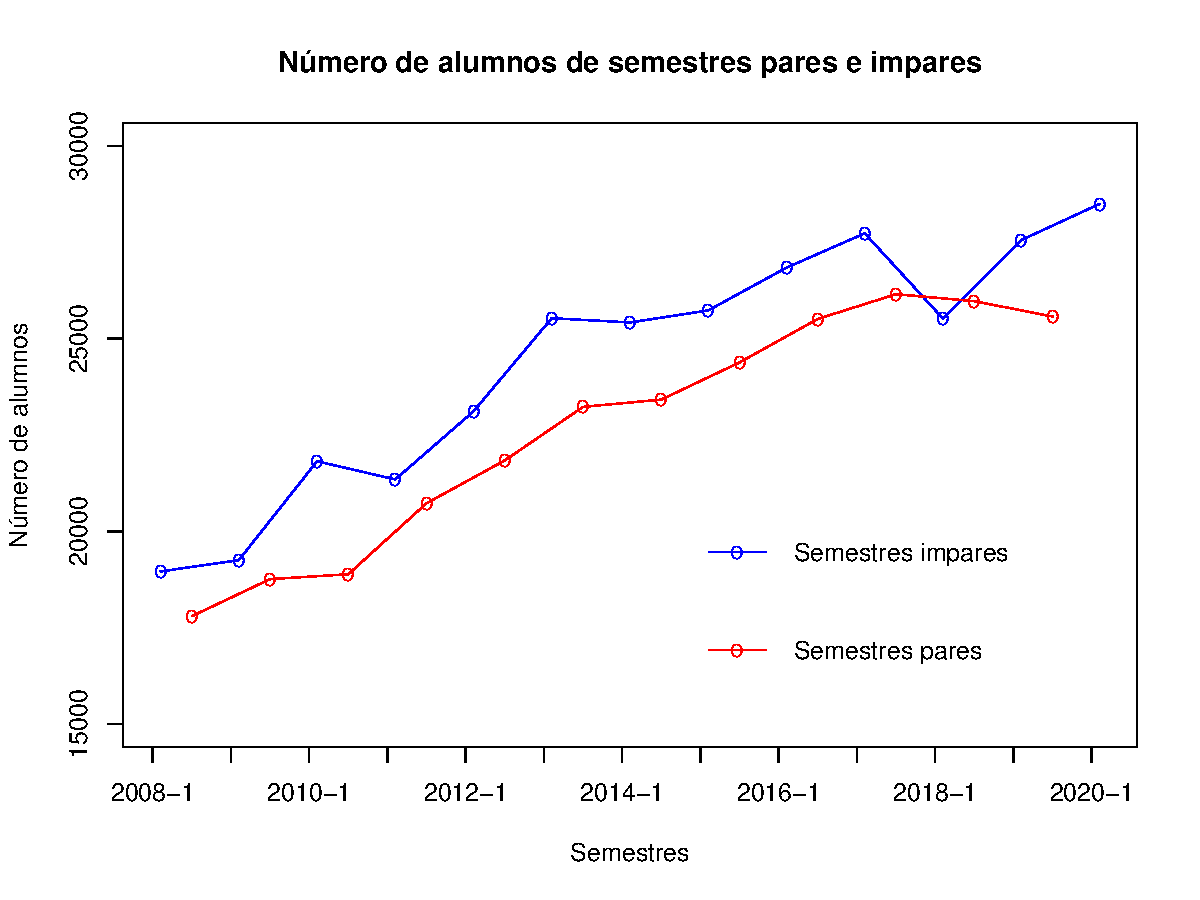
\includegraphics[scale = 0.8]{num_alum_sem_par_impar_ts.pdf} %width=\textwidth
\caption[\textit{Número de alumnos de semestres pares e impares}]{\textit{Número de alumnos de semestres pares e impares: Se observa una tendencia creciente y en general el número de alumnos de semestres impares (línea azul) es mayor al número de alumnos de semestres pares (línea roja).}}\label{NumAlTotal_ParImpar_ts}
\end{figure}


En la \figurename{~\ref{histNumAlTotal_ParImpar}} observamos los dos histogramas con el número total de alumnos de semestres pares e impares con sus respectivas densidades ajustadas. Notamos que hay una ligera diferencia entre el número de alumnos de los semestres pares con respecto al número de alumnos de los semestres impares. Existe una mayor cantidad de grupos en los semestres pares con un menor número de alumnos, que en los semestres impares. Hay una mayor cantidad de grupos en los semestres impares contra los semestres pares, que tienen entre 35 y 100 alumnos. Tanto para los semestres pares como para los impares, el comportamiento de las densidades ajustadas es muy parecido.

\begin{figure}[H]
\centering
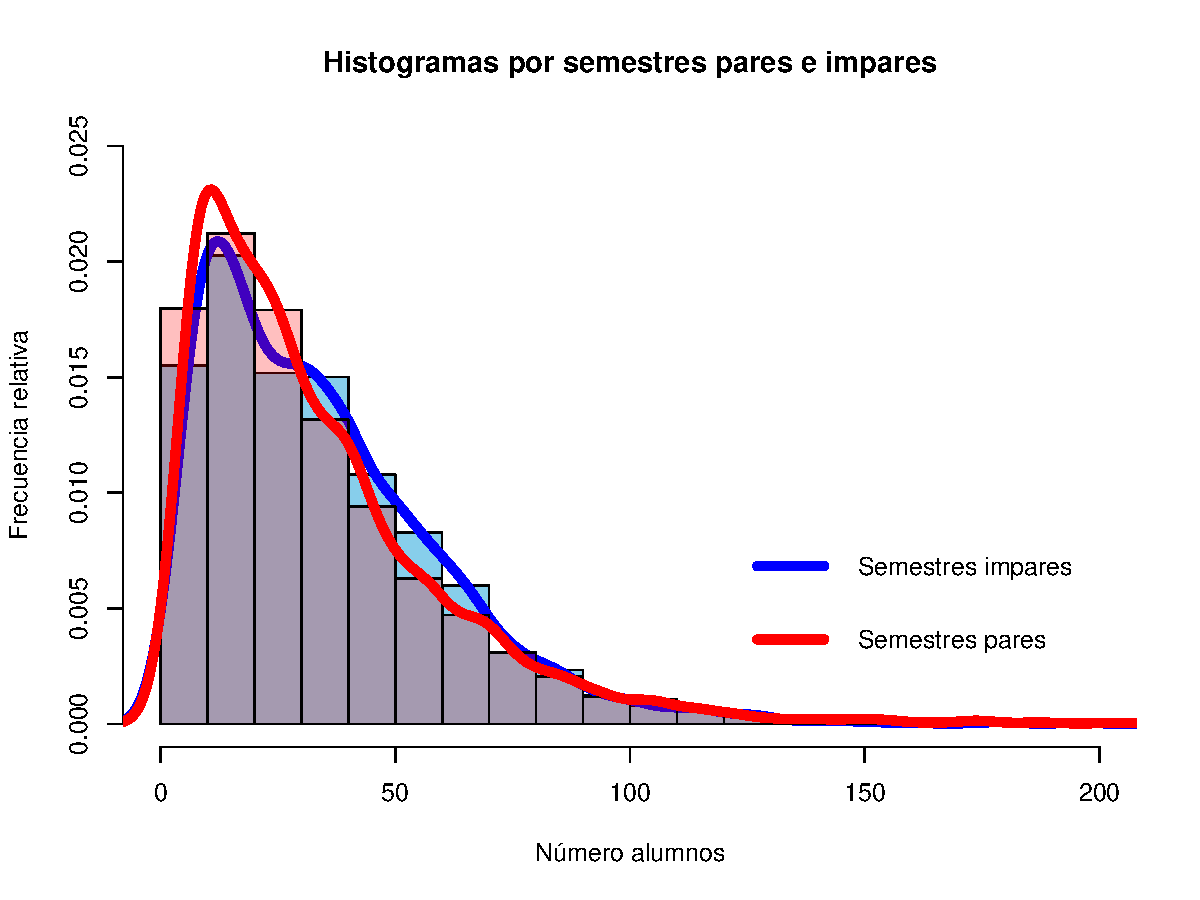
\includegraphics[scale = 0.6]{histograma_FR_num_alum_sem_par_impar.pdf} %width=\textwidth
\caption[\textit{Histogramas del número de alumnos de semestres pares e impares}]{\textit{Histogramas del número de alumnos de semestres pares e impares: Las densidades ajustadas son muy parecidas, no importa si los datos son de semestres pares o impares.}}\label{histNumAlTotal_ParImpar}
\end{figure}


En la \figurename{~\ref{NumAlTotal_MatuVesp_ts}} mostramos la gráfica del número de alumnos por turno: matutino y vespertino. Se puede observar que en todo momento el número de alumnos del turno matutino es mayor al número de alumnos del turno vespertino.

\begin{figure}[H]
\centering
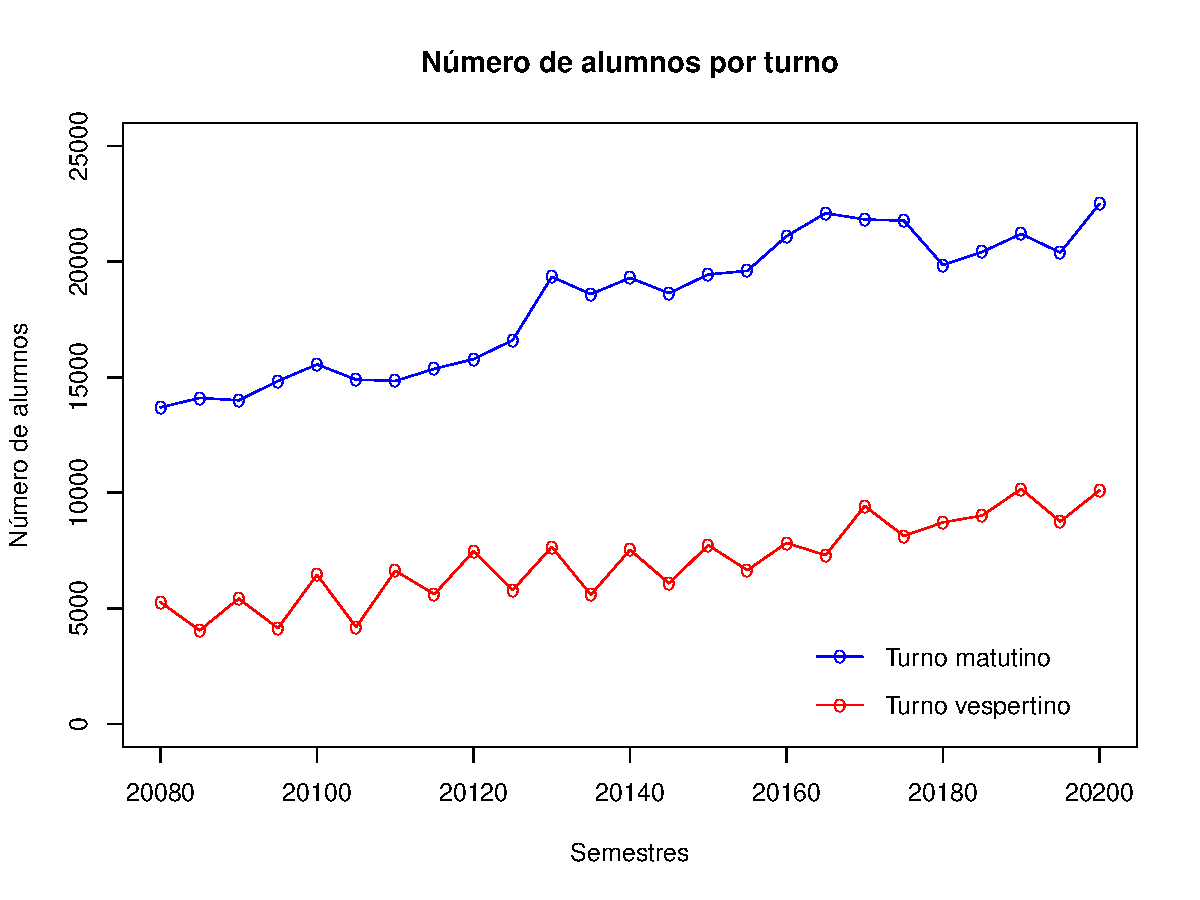
\includegraphics[scale = 0.6]{num_alum_matu_vesp_ts.pdf} %width=\textwidth
\caption[\textit{Número de alumnos por turno de todos los semestres}]{\textit{Número de alumnos por turno de todos los semestres: Se observa que la línea azul (turno matutino) está en todo momento por encima de la línea roja (turno vespertino).}}\label{NumAlTotal_MatuVesp_ts}
\end{figure}

Los datos que se graficaron en el histograma de la \figurename{~\ref{histNumAlTotal_MatuVesp}} son los alumnos totales por hora de cada semestre. En dicha figura se muestran los dos histogramas con los datos divididos en los turnos matutino y vespertino. Notamos que las densidades ajustadas de cada turno son completamente diferentes. Al ver la gráfica podemos concluir que hay más alumnos en el turno matutino que en el vespertino.

\begin{figure}[H]
\centering
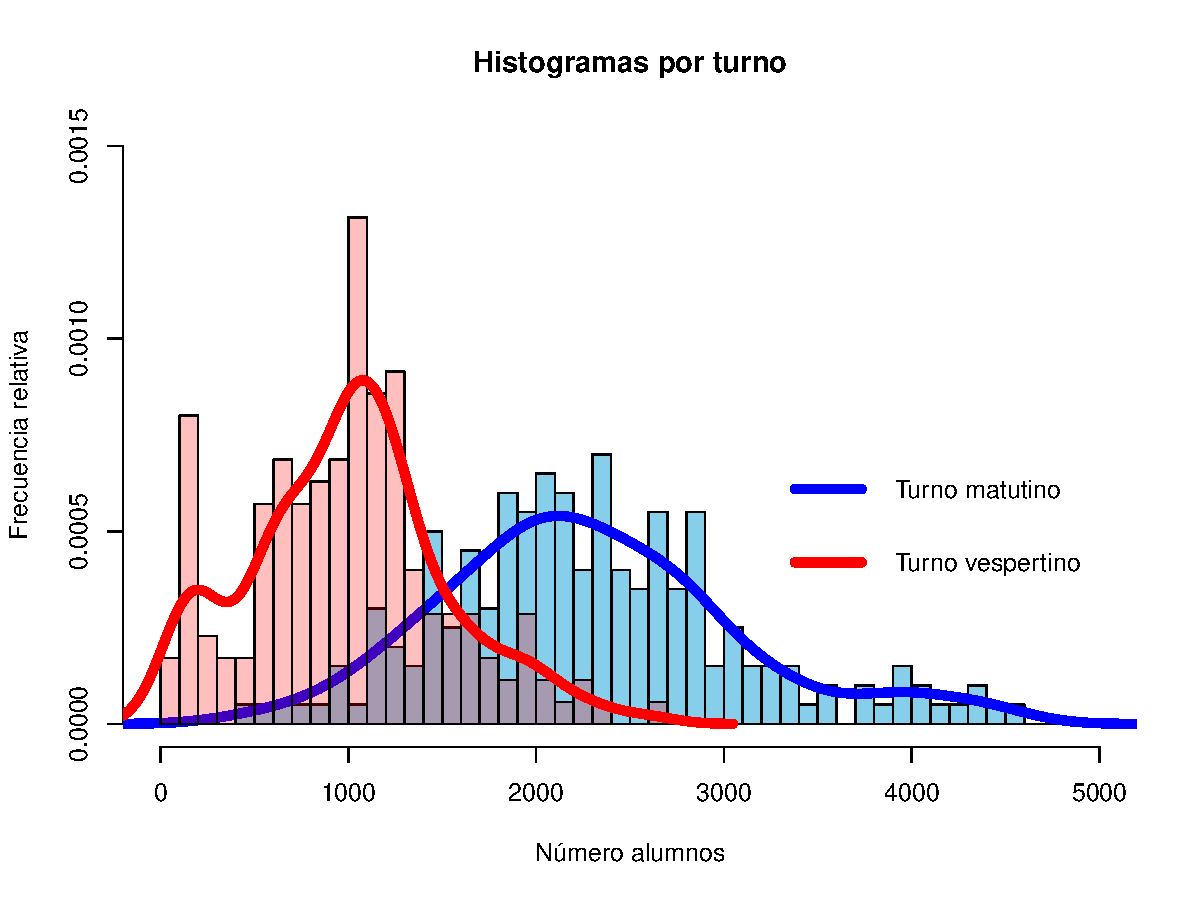
\includegraphics[width=\textwidth]{histograma_FR_num_alum_matu_vesp.pdf} %scale = 0.8
\caption[\textit{Histogramas del número de alumnos de los turnos matutino y vespertino}]{\textit{Histogramas del número de alumnos de los turnos matutino y vespertino: Al observar esta figura podemos concluir que hay más alumnos en el turno matutino que en el vespertino. Sus densidades ajustadas son diferentes.}}\label{histNumAlTotal_MatuVesp}
\end{figure}


\section{Análisis estadístico por carrera}

Es importante recordar que dentro de las carreras existe un tronco común. Es decir, comparten muchas de las materias impartidas en los primeros 4 semestres, por lo que muchos de los grupos de una carrera se encuentran en otra. Cabe mencionar que el número máximo de alumnos por grupo para la carrera de Ciencias de la Computación es 211 y para las otras carreras es 353.

En la \figurename{~\ref{histFAnumAl_x_carrera}} vemos cuatro histogramas con el número de alumnos por grupo, uno para cada carrera del Departamento de Matemáticas. La escala del eje $Y$ es igual para todos los histogramas. De esta manera podemos observar que en las carreras de Actuaría, Ciencias de la Computación y Matemáticas, se tiene la mayor concentración en los grupos de entre 10 y 20 alumnos. La carrera de Matemáticas Aplicadas tiene su mayor concesntración en los grupos que tienen entre 20 y 30 alumnos.

\begin{figure}[H]
\centering
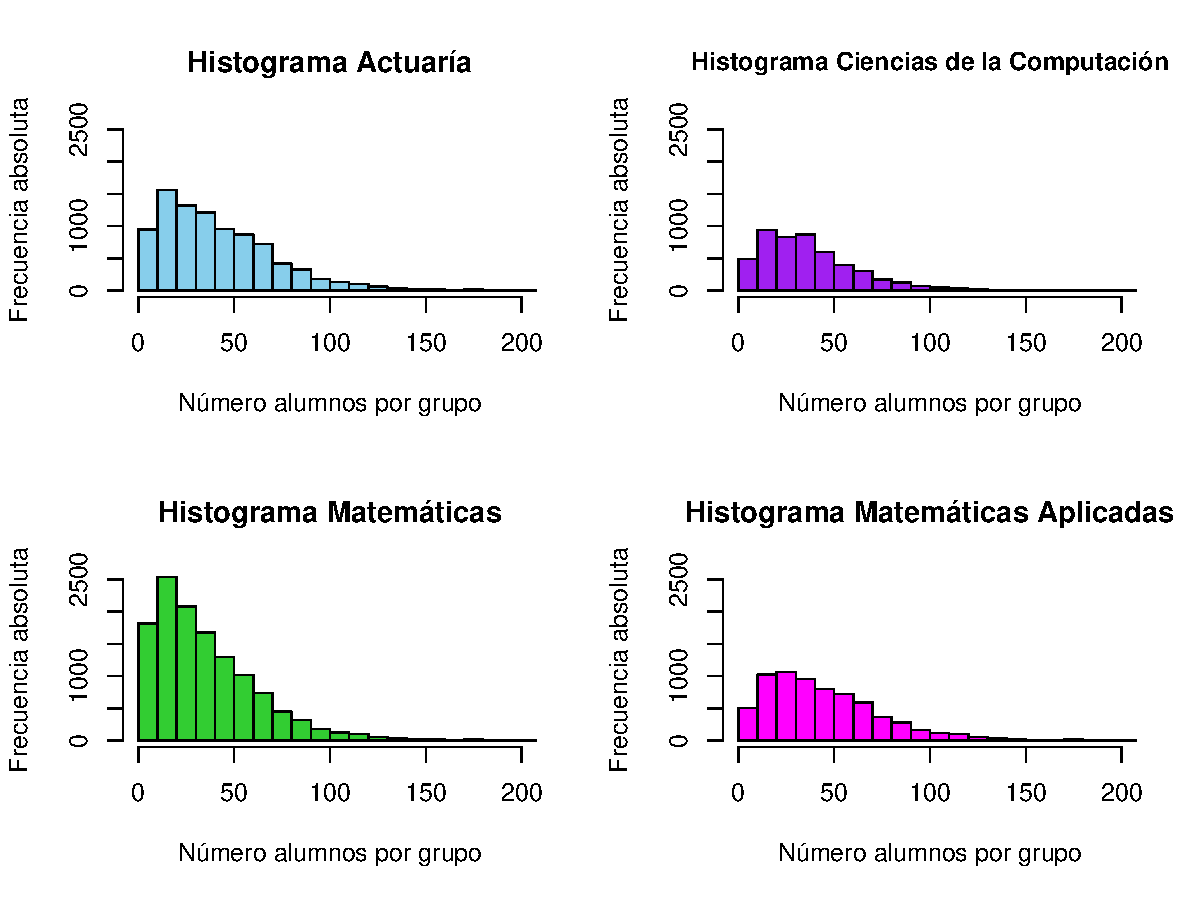
\includegraphics[width=\textwidth]{histogramas_FA_num_alum_x_carrera.pdf} %scale = 0.6
\caption[\textit{Histogramas del número de alumnos por carrera}]{\textit{Histogramas del número de alumnos por carrera: Se muestran los histogramas con el número de alumnos por grupo. Hay un histograma para cada carrera del Departamento de Matemáticas.}}\label{histFAnumAl_x_carrera}
\end{figure}


En la \figurename{~\ref{histFRnumAl_x_carrera}} vemos una gráfica con las densidades ajustadas a los datos del número de alumnos por grupos para cada carrera. Al ver la densidad ajustada a los datos de la carrera de Matemáticas vemos que tiene una mayor concentración de grupos que tienen aproximadamente entre 10 y 30 alumnos, a diferencia de las otras carreras. También podemos observar que en Actuaría y en Matemáticas Aplicadas hay una mayor concentración en los grupos que tienen aproximadamente entre 50 y 75 alumnos, que en Matemáticas o en Ciencias de la Computación. Si vemos la densidad ajustada a los datos de Ciencias de la Computación notamos que hay dos grandes concentraciones, una en los grupos de aproximadamente entre 20 y 30 alumnos y otra entre 40 y 50 alumnos. Con esta gráfica podemos ver con mayor claridad lo que observamos en la \figurename{~\ref{histFAnumAl_x_carrera}}, el comportamiento es similar para todas las carreras pero cada una tiene su propia distribución.

\begin{figure}[H]
\centering
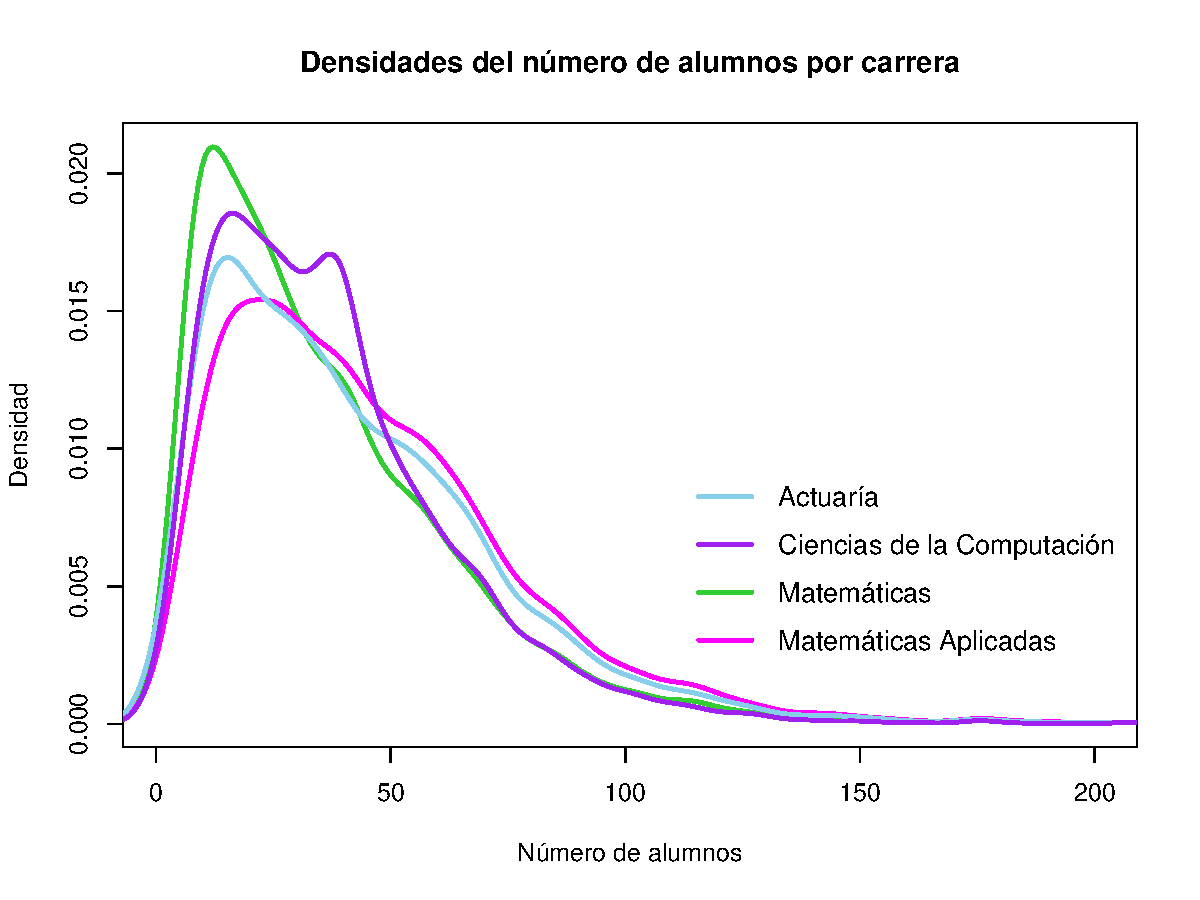
\includegraphics[scale = 0.55]{histogramas_FR_num_alum_x_carrera.pdf} %width=\textwidth
\caption[\textit{Densidades del número de alumnos por carrera}]{\textit{Densidades del número de alumnos por carrera: Se muestran las densidades ajustadas para cada carrera del Departamento de Matemáticas.}}\label{histFRnumAl_x_carrera}
\end{figure}


%\section{Distribución del número de alumnos por grupo / tamaño de grupo}
\section{Distribución del tamaño de los grupos} \label{DitribTamGpos}

En la \figurename{~\ref{histNumAl_x_gpo_x_sem}} se muestra el histograma del número de alumnos por grupo de todos los semestres, desde el 2008-1 hasta el 2020-1. Observamos el mismo comportamiento que en las Figuras \ref{histNumAlTotal_ParImpar}, \ref{histFAnumAl_x_carrera} y \ref{histFRnumAl_x_carrera}. La mayor frecuencia se encuentra en los grupos que tienen entre 10 y 20 alumnos.

\begin{figure}[H]
\centering
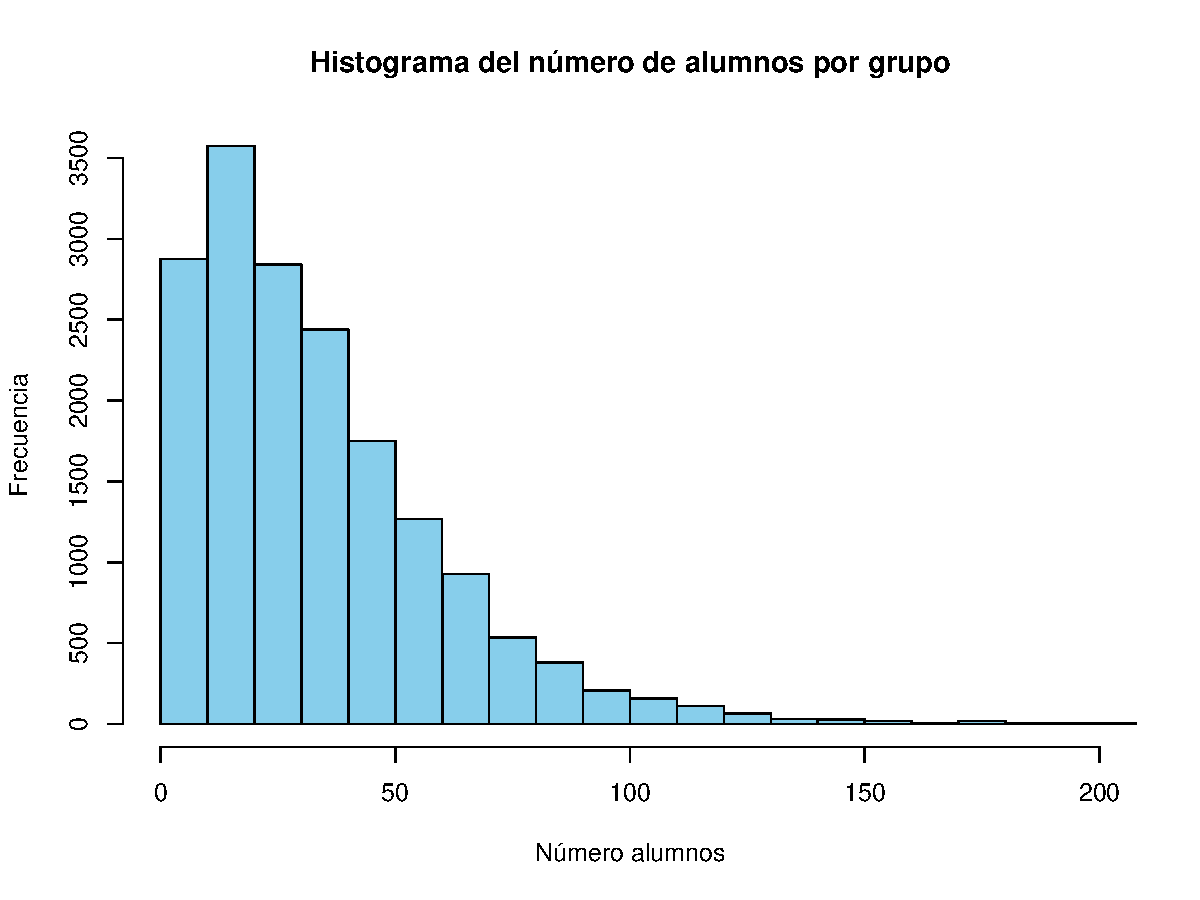
\includegraphics[scale = 0.5]{histograma_FA_num_alum_x_gpo_x_sem.pdf} %width=\textwidth
\caption[\textit{Histograma del número de alumnos por grupo de todos los semestres}]{\textit{Histograma del número de alumnos por grupo de todos los semestres: La información es de los semestres del 2008-1 al 2020-1. Vemos una mayor concentración en los grupos que tienen entre 10 y 40 alumnos.}}\label{histNumAl_x_gpo_x_sem}
\end{figure}


En la \figurename{~\ref{densidadesNumAl_x_gpo_x_sem}} vemos diferentes líneas con las densidades ajustadas a los valores del número de alumnos por grupo de cada semestre. Cada línea corresponde a un semestre. Se tomaron los datos de 25 semestres, del 2008-1 al 2020-1. Notamos que el comportamiento va cambiando conforme pasa el tiempo.

En dicha figura, las líneas de color verde corresponden a las densidades ajustadas a los datos de los semestres del 2008-1 al 2012-2. Las de color rosa corresponden a los semestres del 2013-1 al 2017-2. Las de color azul corresponden a los semestres 2018-1 al 2020-1.

Vemos que en los semestres más antiguos se tiene una concentración mayor en los grupos que tienen aproximadamente entre 10 y 30 alumnos. En los semestres más recientes la mayor concentración se tiene en los grupos con aproximadamente entre 25 y 50 alumnos. Esto lo podemos explicar con el hecho de que cada semestre incrementa el número de alumnos inscritos en la facultad, por lo tanto el tamaño de los grupos aumenta.

También podemos observar que conforme pasa el tiempo la media y la varianza aumentan. Es decir, en semestres antiguos se tiene una menor media y varianza. Ésto comparado con los semestres más actuales, los cuales tienen una media y varianza mayor.

\begin{figure}[H]
\centering
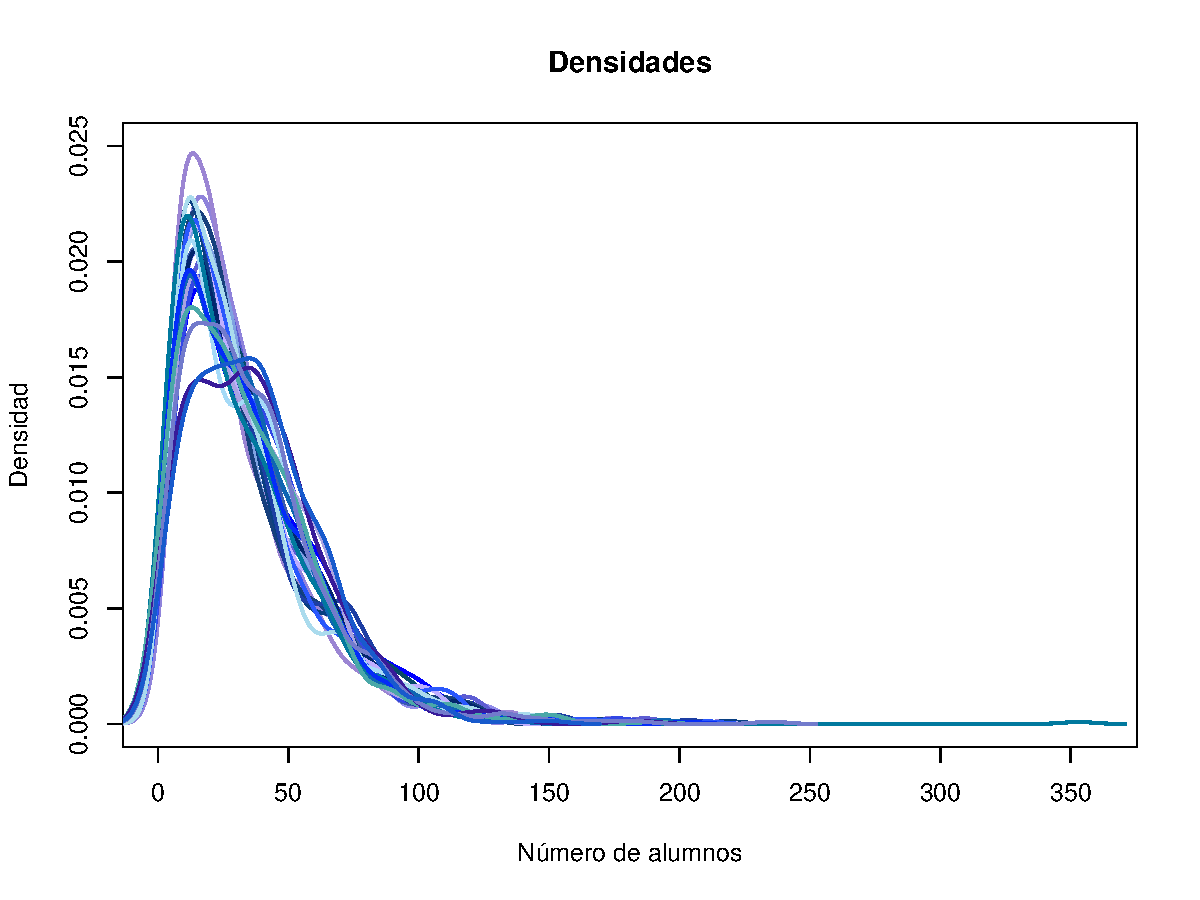
\includegraphics[scale = 0.8]{densidades_num_alum_x_gpo_x_sem.pdf} %width=\textwidth
\caption[\textit{Densidades del número de alumnos por grupo de cada semestre}]{\textit{Densidades del número de alumnos por grupo de cada semestre: Cada línea corresponde a la densidad ajustada de los datos de un semestre entre el 2008-1 y el 2020-1}}\label{densidadesNumAl_x_gpo_x_sem}
\end{figure}

En los semestres del 2013-1 al 2017-2 se tuvieron grupos con más de 350 alumnos. En los semestres más recientes el número máximo de alumnos por grupo fue alrededor de 250. Esto lo podemos explicar por las medidas que se tomaron después del sismo del 19 de septiembre de 2017, con respecto al tamaño de los grupos. El número de alumnos inscritos no podía ser mayor al número de lugares disponibles por salón.

Viendo las Figuras \ref{histNumAl_x_gpo_x_sem} y \ref{densidadesNumAl_x_gpo_x_sem}, podríamos concluir que la distribución que mejor se ajusta al tamaño de los grupos es la distribución Poisson por la forma en la que están distribuidos los datos. Para probar esta hipótesis utilizamos la función \verb@ks.test(X,Y)@, de \textit{R}, para hacer la prueba de Kolmogorov-Smirnov.

La prueba de Kolmogorov-Smirnov, dice que se rechaza $H_{0}$ cuando $D_{n} > D_{n}^{1-\alpha}$. Donde $D_{n}^{1-\alpha}$ nos indica el valor en donde inicia la región de rechazo para un nivel de significancia de $\alpha$ y $n$ es el número de datos de la muestra. Tomamos como hipótesis nula $H_{0}: X$ y $Y$ tienen la misma distribución.

Definimos a $X$ como el vector con el número de alumnos por cada grupo del semestre 2008-1 al 2020-1. Definimos a $Y$ como un vector de números aleatorios de una distribución $Poisson(\lambda)$. Por el resultado \ref{EMVlambda}, del apéndice \ref{Apend_ResultadosUtiles}, sabemos que el estimador máximo verosímil de $\lambda$ para la distribución $Poisson(\lambda)$ es la media de los datos. Con este estimador $(\hat{\lambda} = 34.18),$ obtuvimos los números aleatorios de $Y$. Tenemos que $Y \sim Poisson(34.18)$.%\hat{\lambda} = 34.18746

Por [\ref{Miller}] sabemos que:
  
  \begin{equation}\label{Dn_KS}
D_{n}^{1-\alpha} = \sqrt{\dfrac{ln \left(\dfrac{1}{\alpha}\right)}{2n}} - 1.6693 n^{-1} - 0.20562 n^{-\frac{3}{2}}
\end{equation}

En nuestro caso los valores de las variables son: $n = 17,246$ y $\alpha = 0.01$. Sustituyendo en la ecuación \ref{Dn_KS} tenemos que $D_{17246}^{0.99} = 0.01$. Con la función \verb@ks.test(X,Y)@, de \textit{R}, obtenemos el valor de $D_{17246} = 0.39$.

Como $D_{17246} = 0.39 > 0.01 = D_{17246}^{0.99}$, entonces se rechaza $H_{0}$, por lo tanto los datos no siguen una distribución Poisson con $\lambda = 34.18$.


Hicimos otra prueba suponiendo que los datos tienen una distribución $Normal(\mu,\sigma)$. Para simular los datos de $Y$ utilizamos los estimadores máximo verosímiles de $\mu$ y $\sigma$. Estos estimadores los obtuvimos con la función \verb@fitdistr(X, densfun="normal")@, en \textit{R}. Los valores de los estimadores son $\hat{\mu} = 34.18$ y $\hat{\sigma} = 26.57$. El resultado de la función de la prueba de Kolmogorov-Smirnov es $D_{17246} = 0.10$.

Como $D_{17246} = 0.10 > 0.01 = D_{17246}^{0.99}$, entonces se rechaza $H_{0}$, por lo tanto los datos no siguen una distribución $Normal(34.18,26.57)$.

Hicimos más pruebas con otras distribuciones y en todos los casos rechazamos la hipótesis nula. En la \figurename{~\ref{histFR_pruebaKS}} vemos únicamente los casos que expusimos en esta sección. El histograma representa las frecuencias relativas de los datos del número de alumnos por grupo para cada semestre. La línea azul es la densidad ajustada generada por \textit{R}, la línea morada es la densidad de $n$ números aleatorios con distribución  $Poisson(34.18)$ y la línea roja es la densidad de $n$ números aleatorios con distribución  $Normal(34.18,26.57)$.

%Hicimos más pruebas con otras distribuciones y en todos los casos rechazamos la hipótesis nula. Con estos resultados concluímos que el ajuste que se pudiera hacer a los datos tendría que ser en dos partes. Un ejemplo de una posible partición de los datos es que se puede ajustar una distribución para los datos que están entre 0 y 100, y otra distribución para los datos mayores a 100. Esto debido a que a pesar de ser pocos los datos mayores a 100, si impactan en la distribución total. El análisis con esta propuesta no lo realizamos para este trabajo.

\begin{figure}[H]
\centering
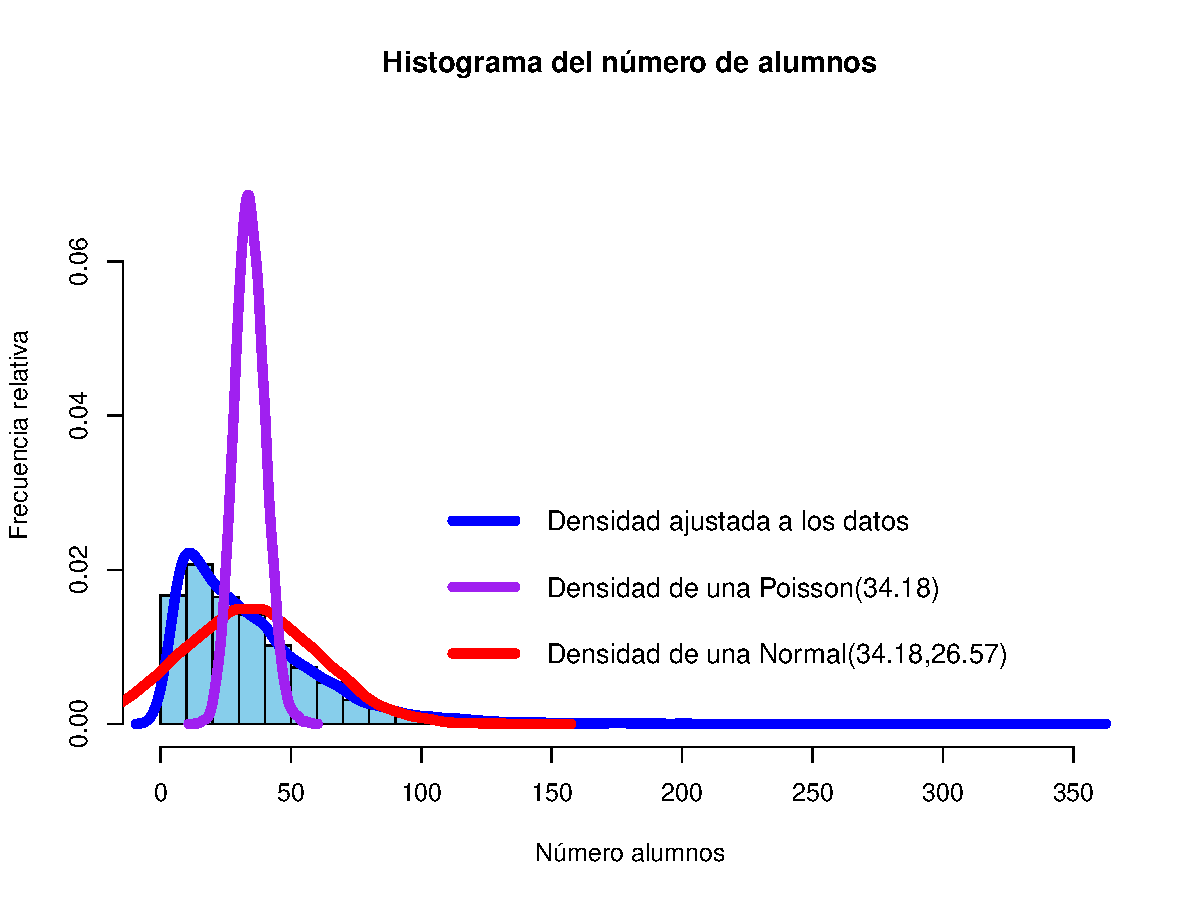
\includegraphics[scale = 0.8]{histograma_FR_prueba_KS.pdf} %width=\textwidth
\caption[\textit{Histograma con densidades ajustadas}]{\textit{Histograma con densidades ajustadas: Se muestran 3 densidades ajustadas. La línea azul es la ajustada con el método kernel gaussiano por la función $\mathrm{density()}$. La morada corresponde a una Poisson(34.18). La roja corresponde a una Normal(34.18,26.57). Ninguna de las distribuciones propuestas se ajustan de manera adecuada a los datos.}}\label{histFR_pruebaKS}
\end{figure}

%Hicimos más pruebas con otras distribuciones y en todos los casos rechazamos la hipótesis nula. Con estos resultados concluímos que el ajuste que se pudiera hacer a los datos tendría que ser en dos partes. Un ejemplo de una posible partición de los datos es que se puede ajustar una distribución para los datos que están entre 0 y 100, y otra distribución para los datos mayores a 100. Esto debido a que a pesar de ser pocos los datos mayores a 100, si impactan en la distribución total. El análisis con esta propuesta no lo realizamos para este trabajo.


\section{Comportamientos por hora}

En esta sección veremos algunas gráficas cuyo eje $x$ corresponde a las horas en las que se imparten las clases. Se empieza por la clase de 7-8hrs y se termina con la clase de 21-22hrs. Primero mostraremos el comportamiento del promedio de grupos por hora y después el comportamiento del promedio del número de alumnos por hora.

En la \figurename{~\ref{num_prom_gpos_x_hora_barplot}} vemos la gráfica de barras con el número promedio de grupos por hora. Tomamos la información de 25 semestres. Observamos una disminución considerable del número de grupos a las 15hrs. Podemos concluir que es debido a que a esa hora, usualmente la gente sale a comer. A las 21hrs se tiene el menor número de grupos, esto se puede explicar por el hecho de que es la última clase impartida en la Facultad.

Hay un descenso leve a las 9hrs donde se pudiera suponer que la gente sale a desayunar. Desde las 7hrs se pueden encontrar clases como \textit{Cálculo Diferencial e Integral}. Pero en general, las clases impartidas a las 7hrs y a las 8hrs suelen ser materias exclusivas para los actuarios como \textit{Teoría del Seguro, Matemáticas Actuariales del Seguro de Personas I y II} o \textit{Matemáticas Actuariales para Seguro de Daños, Fianzas y Reaseguro}. Podemos decir que a partir de las 9 de la mañana se imparten materias de todas las carreras.

%Hay un descenso leve a las 9hrs donde se pudiera suponer que la gente sale a desayunar. En mi caso particular, al estudiar la carrera de Actuaría, tenía clases desde las 7a.m. por lo que las 9a.m. era una buena hora para hacer una pequeña pausa en el horario y tener un descanso para desayunar. Esta hora coincide con el cambio en el que se dejan de impartir las materias exclusivas para los actuarios como Teoría del Seguro, MASP o MASD. Es decir, a partir de las 9 de la mañana se imparten materias de todas las carreras.

A las 10 de la mañana se tiene el número máximo de grupos. Con esta información se podría medir la capacidad que debería de tener la Facultad en cuanto al número de salones necesarios para cubrir la demanda de grupos. Si se está preparado para cubrir la demanda del pico más alto de todas las horas, entonces los demás casos están cubiertos por tener un menor número de grupos.


\begin{figure}[H]
\centering
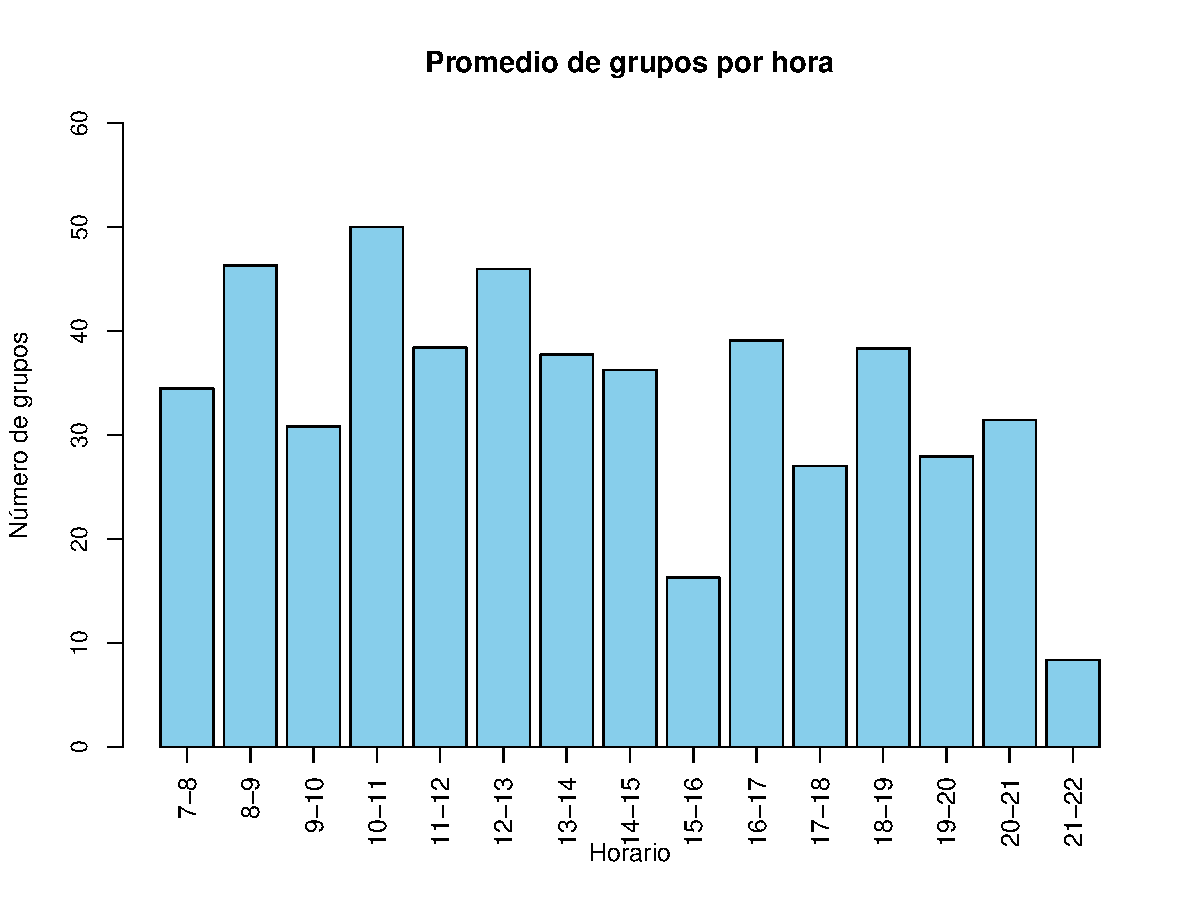
\includegraphics[scale = 0.8]{num_prom_gpos_x_hora_barplot.pdf} %width=\textwidth
\caption[\textit{Número promedio de grupos por hora}]{\textit{Número promedio de grupos por hora: Se observa una disminución considerable a las 15hrs y a las 21hrs. El valor más alto se encuentra a las 10hrs.}}\label{num_prom_gpos_x_hora_barplot}
\end{figure}

En la \figurename{~\ref{prom_alum_x_hora_barplot}} se muestra la gráfica de barras con el promedio del número de alumnos por hora. Notamos que el comportamiento de ésta gráfica es muy similar al de la gráfica mostrada en la \figurename{~\ref{num_prom_gpos_x_hora_barplot}}. El pico más alto de los datos también se tiene a las 10 de la mañana y el menor número de alumnos se encuentra a las 21hrs. También hay una disminución considerable a las 15hrs.

\begin{figure}[H]
\centering
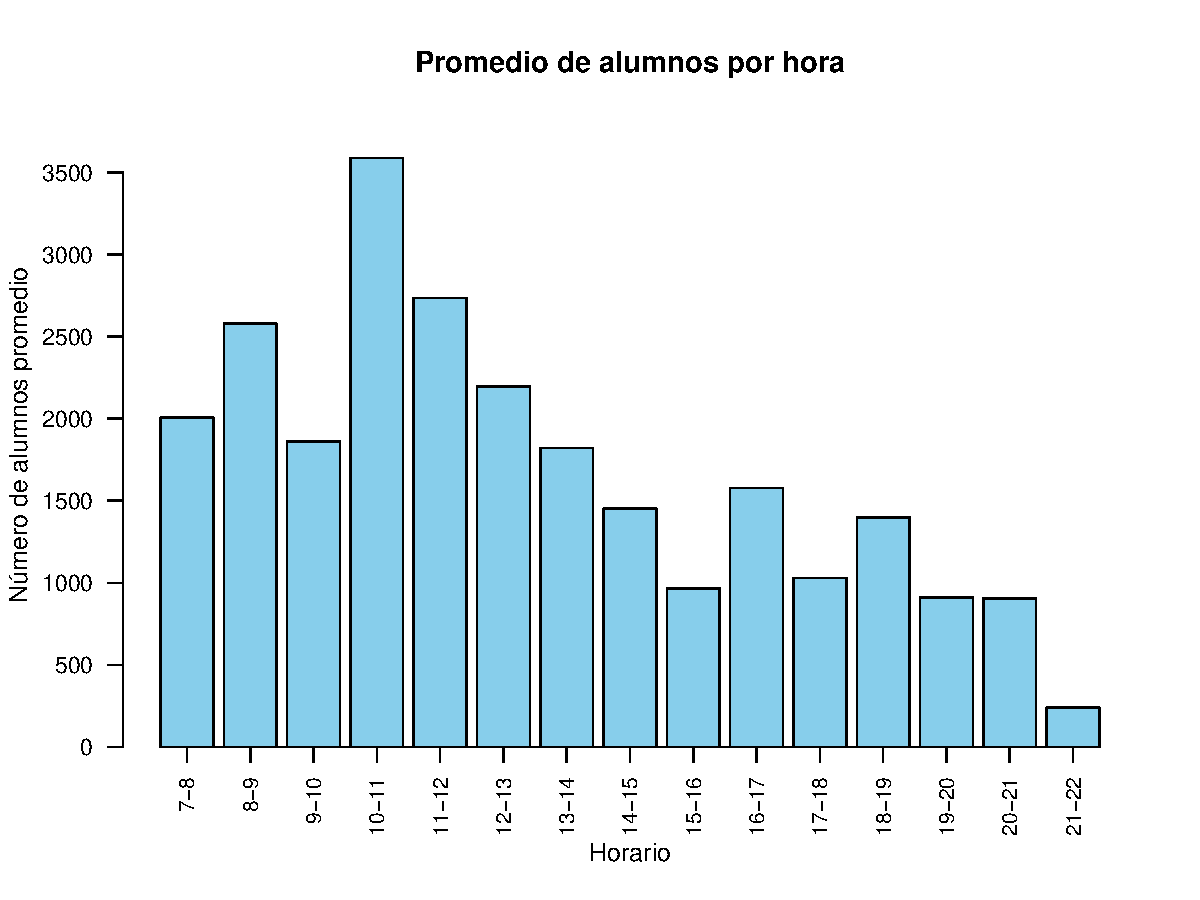
\includegraphics[scale = 0.8]{prom_alum_x_hora_barplot.pdf} %width=\textwidth
\caption[\textit{Número promedio de alumnos por hora}]{\textit{Número promedio de alumnos por hora: Notamos una disminución de los valores a las 9hrs, a las 15hrs y a las 21hrs. El valor más alto lo encontramos a las 10hrs.}}\label{prom_alum_x_hora_barplot}
\end{figure}

Viendo las Figuras \ref{num_prom_gpos_x_hora_barplot} y \ref{prom_alum_x_hora_barplot} podemos concluir que existe una correlación entre el número promedio de grupos por hora y el número promedio de alumnos por hora. Por ejemplo, si no hay alumnos que tomen clases a las 15hrs entonces no tiene caso que se abran grupos a esa hora. Análogamente para las 21hrs. Por el contrario entre más alumnos haya por hora, se deben abrir más grupos a esas horas, como es el caso de las 10hrs. %%3

\chapter{Simulación}

La simulación es un proceso que nos permite estudiar el comportamiento de un sistema complejo que es muy difícil de examinar de manera analítica. Nos ayuda a determinar de manera empírica las probabilidades de ciertos eventos. La simulación nos permite experimentar con diversos supuestos que podrían ser muy costosos de realizar. Las áreas en las que se utiliza la simulación como herramienta diaria son por ejemplo en biología, estadística, medicina, química, matemáticas, investigación de operaciones, física, ingeniería o en las ciencias sociales.

Algunos ejemplos de su aplicación van desde simular el lanzamiento de una moneda justa, hasta la simulación de colisiones de átomos en un acelerador de partículas. Se utiliza para todo tipo de propósitos, por ejemplo para poder realizar predicciones en base a datos históricos o enseñar a los pilotos a volar un avión sin poner en riesgo a la población al volar el avión real.

Actualmente se combinan diferentes metodologías de simulación con el software disponible, el análisis de sensibilidad y la optimización estocástica para poder obtener un mejor resultado al momento de simular sistemas que se hacen cada vez más complejos como las redes neuronales.

A lo largo de este capítulo explicaremos el proceso que seguimos para obtener la asignación de los horarios para cada materia con su respectivo profesor.

\section{Funciones hechas en R}

El diagrama de flujo de la función \textbf{gen\_asignacion} se puede ver en la figura \ref{DF_genAsig}.

\begin{figure}[H]
\centering
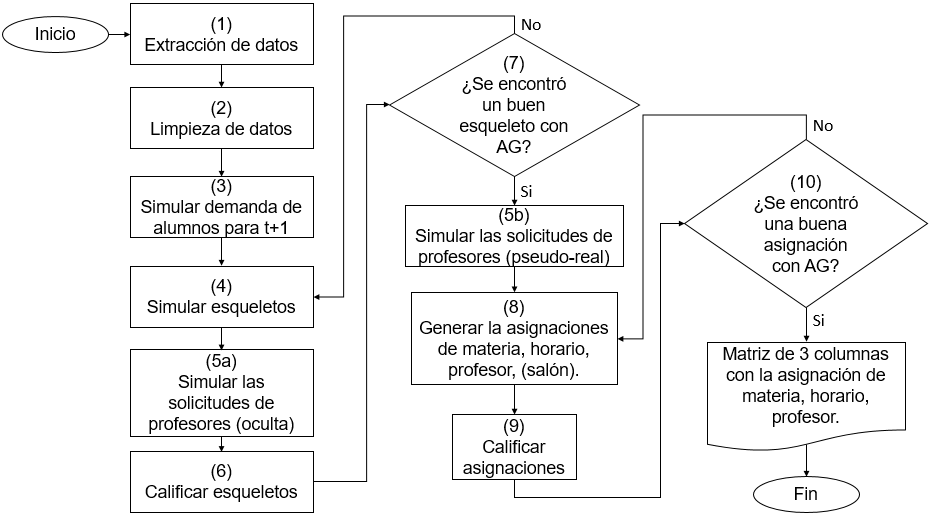
\includegraphics[scale = 0.7]{diagrama_flujo} %width=\textwidth
\caption{\textit{Diagrama de flujo de la función \textbf{gen\_asignacion}}}\label{DF_genAsig}
\end{figure}


\begin{itemize}
\item \textit{posibles\_url}

\item \textit{gen\_m\_grande}

\item \textit{gen\_m\_grande\_total}

\item \textit{gen\_esqueleto: } Función que genera esqueletos la cual carga la función \textit{simula\_grupos} y ésta a su vez carga la función \textit{estima\_grupos}.

\item \textit{gen\_solicitudes}

\item \textit{gen\_asignacion}

\item \textit{gen\_simula\_alumnos}

\item \textit{gen\_simula\_tamano\_grupo}
\end{itemize}

\section{Obtención de los parámetros $q_{1}$ y $q_{2}$}

En esta sección vamos a explicar cómo obtuvimos los valores de $q_{1}$ y $q_{2}$. Son parámetros que se introducen en la función \verb@hw()@ de \textit{R}. Representan los cuantiles utilizados al calcular los intervalos de confianza. Por ejemplo si $q_{1} = 80$ entonces se calcula el intervalo al $80\%$ de confianza. Si se introducen a la función los dos parámetros entonces se calculan dos intervalos, uno al $q_{1}\%$ de confianza y el otro al $q_{2}\%$ de confianza.

Primero definimos los parámetros generales necesarios para las simulaciones:

\begin{enumerate}
\item Fijamos la semilla con \verb@set.seed(8654)@.

\item Elegimos 3 semestres para simular la demanda del número de alumnos. Los seleccionamos de los semestres que ya teníamos guardados con información real. Hicimos una comparación entre nuestros datos simulados y los reales de cada semestre. Los semestres que elegimos fueron: 2019-1, 2019-2 y 2020-1.

\item Fijamos $k = 5$ (número de semestres que se tienen como ventana de información).

\item Fijamos $num\_sim = 10$ (número de simulaciones de la demanda de alumnos para el semestre a simular).
\end{enumerate}


Después fijamos 5 materias que consideramos representativas para hacer las pruebas iniciales: \textit{Cálculo Diferencial e Integral I}, \textit{Demografía I}, \textit{Modelos no Paramétricos y de Regresión}, \textit{Administración de Riesgos Financieros} y \textit{Seminario de Investigación de Operaciones}.

Tomamos 12 posibles combinaciones de valores para $q_{1}$ y $q_{2}$, las cuales podemos ver en la \tablename{\ref{valoresQ1Q2}}. La letra \textit{L} indica que se tomó la cota inferior de $q_{1}$ y la letra \textit{U} indica que se tomó la cota superior de $q_{2}$. Con estas cotas formamos intervalos de los cuales obtuvimos las simulaciones para los 3 diferentes semestres previamente elegidos. %Con las cotas de tipo \textit{$Lq_{1}$,$Uq_{2}$} se forma un intervalo del que s

\begin{table}[H]
\centering
\begin{tabular}{|c|c|c|c|c|}
\hline 
$q_{1} \backslash q_{2}$ & 80 & 85 & 90 & 99 \\ 
\hline 
80 & - & L80,U85 & L80,U90 & L80,U99 \\ 
\hline 
85 & L85,U80 & - & L85,U90 & L85,U99 \\ 
\hline 
90 & L90,U80 & L90,U85 & - & L90,U99 \\ 
\hline 
99 & L99,U80 & L99,U85 & L99,U90 & - \\ 
\hline 
\end{tabular} 
\caption[\textit{Posibles valores para $q_{1}$ y $q_{2}$}]{\textit{Posibles valores para $q_{1}$ y $q_{2}$: Tabla que muestra todas las combinaciones de los intervalos formados con las cotas inferiores y superiores de $q_{1}$ y $q_{2}$}}\label{valoresQ1Q2}
\end{table}


Una vez hecha la simulación obtuvimos una tabla con 7 columnas: materia, intervalo, mín, media, máx, sd y seg. Donde en el renglón i se tienen los datos de la matriz de diferencias relativas de la i-ésima materia para cada intervalo de $q_{1}$ y $q_{2}$. La matriz de diferencias relativas se genera al restar, para cada materia, los datos reales menos los simulados y después dividirlos entre los reales. Por ejemplo en el primer renglón de la \figurename{\ref{matMedDispersion}} vemos que se utilizó el intervalo $(L80,U85)$ para obtener el número de alumnos simulados para el siguiente semestre de la materia \textit{Cálculo Diferencial e Integral I}. Las columnas 2, 3, 4 y 5 corresponden a las medidas de la matriz de diferencias relativas para cada materia. La última columna indica el tiempo que se tardó el proceso.

\begin{figure}[H]
\centering
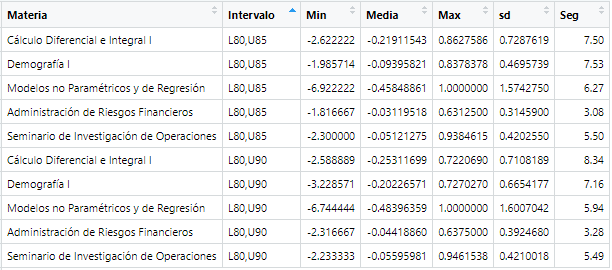
\includegraphics[scale = 0.9]{mat_med_dispersion} %width=\textwidth
\caption[\textit{Matriz con información por materia}]{\textit{Matriz con información por materia: vemos los primeros 10 renglones de la tabla obtenida con información de la matriz de diferencias relativas.}}\label{matMedDispersion}
\end{figure}


Decidimos elegir $q_{1}$ y $q_{2}$ en base a la desviación estándar. Con la \figurename{\ref{matMedDispersion}} obtuvimos una matriz de dos columnas que contine en su primer columna el intervalo y en la segunda el promedio de la desviación estándar para cada intervalo de las 5 materias. Los datos de dicha matriz los podemos ver en la \figurename{\ref{promSD_5m_12p}}.

\begin{figure}[H]
\centering
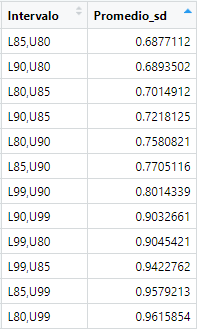
\includegraphics[scale = 1]{prom_SD_5m_12p} %width=\textwidth
\caption[\textit{Promedio de la desviación estándar: 5 materias, 12 pruebas}]{\textit{Promedio de la desviación estándar: 5 materias, 12 pruebas: Matriz con el promedio de la desviación estándar para 5 materias y 12 diferentes intervalos.}}\label{promSD_5m_12p}
\end{figure}


Los datos en la \figurename{\ref{promSD_5m_12p}} están ordenados de menor a mayor con respecto al promedio de la desviación estándar. Para la segunda prueba se eligieron los primeros 6 intervalos de dicha tabla. Se eligieron 10 materias: \textit{Álgebra Lineal I}, \textit{Álgebra Superior II}, \textit{Algoritmos Genéticos}, \textit{Análisis Matemático IV}, \textit{Análisis Numérico}, \textit{Teoría de la Medida I}, \textit{Cálculo Diferencial e Integral IV}, \textit{Graficas y Juegos}, \textit{Inglés I} y \textit{Matemáticas Actuariales para Seguro de Daños}. La tabla con el promedio de la desviación estandar de sus datos se puede ver en la \figurename{\ref{promSD_10m_6p}}.


\begin{figure}[H]
\centering
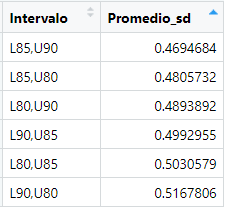
\includegraphics[scale = 1]{prom_SD_10m_6p} %width=\textwidth
\caption[\textit{Promedio de la desviación estándar: 10 materias, 6 pruebas}]{\textit{Promedio de la desviación estándar: 10 materias, 6 pruebas: Matriz con el promedio de la desviación estándar para 10 materias y 6 diferentes intervalos.}}\label{promSD_10m_6p}
\end{figure}


Para la tercera prueba elegimos, de la \figurename{\ref{promSD_10m_6p}} los intervalos que tuvieran un promedio en la desviación estándar menor a $0.5$. Seleccionamos otras 10 materias: \textit{Estadística III}, \textit{Teoría del Seguro}, \textit{Programación Entera}, \textit{Investigación de Operaciones}, \textit{Geometría Moderna I}, \textit{Geometría Analítica II}, \textit{Lógica Matemática I}, \textit{Cálculo Diferencial e Integral III}, \textit{Estadística I} y \textit{Bases de Datos}. La tabla con el promedio de la desviación estandar de sus datos se puede ver en la \figurename{\ref{promSD_10m_4p}}.


\begin{figure}[H]
\centering
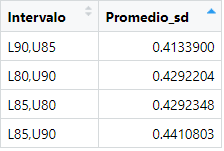
\includegraphics[scale = 1]{prom_SD_10m_4p} %width=\textwidth
\caption[\textit{Promedio de la desviación estándar: 10 materias, 4 pruebas}]{\textit{Promedio de la desviación estándar: 10 materias, 4 pruebas: Matriz con el promedio de la desviación estándar para 10 materias y 4 diferentes intervalos.}}\label{promSD_10m_4p}
\end{figure}

Podemos ver que los valores de la \figurename{\ref{promSD_10m_4p}} son muy parecidos. Hicimos una prueba con los mismos intervalos pero con 5 materias que se dan en todos los semestres y además tienen muchos alumnos. Hicimos la prueba para ver si había alguna diferencia en los datos y poder elegir un sólo intervalo. Las materias que elegimos para esta prueba fueron: \textit{Geometría Analítica I}, \textit{Cálculo Diferencial e Integral II}, \textit{Finanzas I}, \textit{Probabilidad II} y \textit{Procesos Estocásticos I}. La tabla con el promedio de la desviación estandar de sus datos se puede ver en la \figurename{\ref{promSD_5m_4p}}.


\begin{figure}[H]
\centering
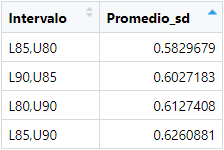
\includegraphics[scale = 1]{prom_SD_5m_4p} %width=\textwidth
\caption[\textit{Promedio de la desviación estándar: 5 materias, 4 pruebas}]{\textit{Promedio de la desviación estándar: 5 materias, 4 pruebas: Matriz con el promedio de la desviación estándar para 5 materias y 4 diferentes intervalos.}}\label{promSD_5m_4p}
\end{figure}

Analizando la información de las matrices de las Figuras \ref{promSD_10m_4p} y \ref{promSD_5m_4p}, decidimos elegir los valores de $q_{1} = 85$ y $q_{2} = 80$. Por lo que el intervalo que buscamos estará formado por la cota inferior del intervalo de confianza al $85\%$ y por la cota superior del intervalo de confianza al $80\%$. Para visualizar de una mejor manera cómo se encuentra el intervalo formado, podemos ver la \figurename{\ref{interConf}}. De ese intervalo vamos a obtener los valores para simular la demanda de alumnos.

\begin{figure}[H]
\centering
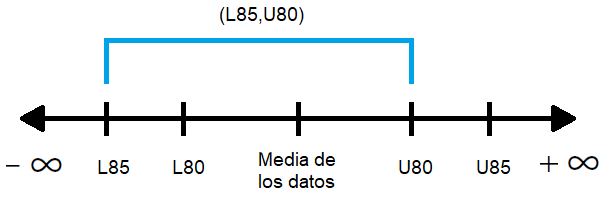
\includegraphics[scale = 0.7]{intervalos_confianza} %width=\textwidth
\caption[\textit{Diagrama de los intervalos de confianza}]{\textit{Diagrama de los intervalos de confianza: Se muestra el intervalo del que se va a obtener el número de alumnos para la simulación de cada materia en cada hora.}}\label{interConf}
\end{figure}

Finalmente con los valores de $q_{1} = 85$ y $q_{2} = 80$ hicimos una prueba aleatoria (eliminando la semilla). Las materias que elegimos para dicha prueba son: \textit{Estadística III}, \textit{Teoría del Seguro}, \textit{Cálculo Diferencial e Integral I}, \textit{Investigación de Operaciones}, \textit{Geometría Moderna I}, \textit{Geometría Analítica II}, \textit{Lógica Matemática I}, \textit{Cálculo Diferencial e Integral III}, \textit{Estadística I}, \textit{Bases de Datos}, \textit{Matemáticas Financieras}, \textit{Cálculo Diferencial e Integral II}, \textit{Probabilidad I}, \textit{Probabilidad II} y \textit{Procesos Estocásticos I}. Los resultados de la prueba aleatoria los podemos ver en la \figurename{\ref{mat_med_dispersion_pruebaAl}}. El promedio de la desviación estándar de todas las materias es $0.48$.%$0.4814898$.

\begin{figure}[H]
\centering
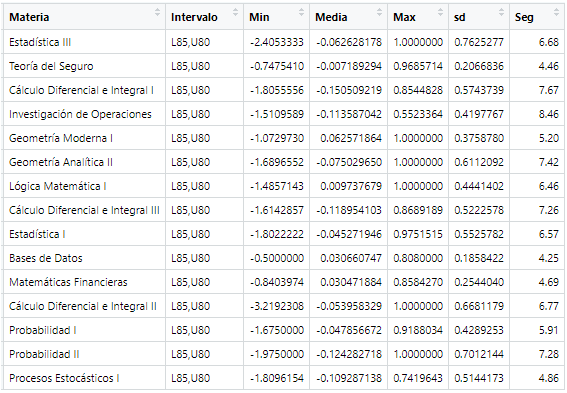
\includegraphics[scale = 0.9]{mat_med_dispersion_pruebaAleatoria} %width=\textwidth
\caption[\textit{Matriz con medidas de dispersión de prueba aleatoria}]{\textit{Matriz con medidas de dispersión de prueba aleatoria: Se muestra en cada renglón la materia y el intervalo del que se tomaron los valores para la simulación.}}\label{mat_med_dispersion_pruebaAl}
\end{figure}
 %%Subsección %%To include subfiles in to a subfiles use \input{name_of_file}

\section{Simulación de la demanda de alumnos}

La demanda del número de alumnos para el siguiente semestre la hicimos por materia y por hora. Para poder hacer la simulación lo primero que hicimos fue acomodar la información que teníamos por semestres y por hora. El procedimiento que seguimos es el siguiente:

\begin{enumerate}
\item Definir el semestre del cual se quiere obtener la simulación.

\item Definir el número de semestres que se quieren como ventana de información.

\item Tomar una submatriz de \textit{m\_grande\_total} con la información de una materia para los semestres en la ventana de información.

\item Para cada semestre dentro de la ventana de información se suma el número de alumnos en cada hora.

\item Se obtiene una matriz de $15 \times k$ ($k$ es el número de semestres en la ventana) como la que se puede ver en la figura \ref{matAl_corregidos}.
\end{enumerate}

%Por ejemplo si teníamos en el semestre 2018-2 una matriz como la que se muestra en la tabla \ref{TablaVariasMaterias} entonces por cada hora sumamos los datos y así para cada semestre.
%\begin{table}[h]
%\centering
%\begin{tabular}{|c|c|c|}
%\hline 
%Horario & Materia 1 & Materia 2 \\ 
%\hline 
%7-8 & 0 & 0 \\ 
%\hline 
%8-9 & 0 & 0 \\ 
%\hline 
%9-10 & 0 & 0 \\ 
%\hline 
%10-11 & 0 & 0 \\ 
%\hline 
%11-12 & 11 & 33 \\ 
%\hline 
%12-13 & 45 & 30 \\ 
%\hline 
%13-14 & 0 & 0 \\ 
%\hline 
%14-15 & 0 & 0 \\ 
%\hline 
%15-16 & 0 & 0 \\ 
%\hline 
%16-17 & 0 & 0 \\ 
%\hline 
%17-18 & 30 & 22 \\ 
%\hline 
%18-19 & 0 & 0 \\ 
%\hline 
%19-20 & 0 & 0 \\ 
%\hline 
%20-21 & 18 & 35 \\ 
%\hline 
%21-22 & 0 & 0 \\ 
%\hline
%\end{tabular} 
%\caption{\textit{Ejemplo de información varias materias}}\label{TablaVariasMaterias}
%\end{table}
%Podemos ver un ejemplo de la matriz que se formó, al aplicar el procedimiento descrito, para varios semestres, en la figura \ref{matAl_corregidos}.

\begin{figure}[H]
\centering
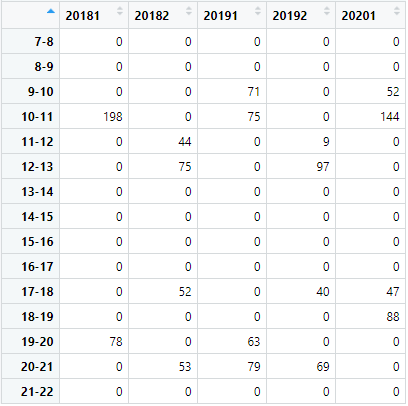
\includegraphics[scale = 0.8]{mat_alumnos_corregidos_EstadisticaIII} %width=\textwidth
\caption{\textit{Ejemplo de matriz con alumnos corregidos}}\label{matAl_corregidos}
\end{figure}

Con el procedimiento descrito pudimos generar vectores por hora y aplicar la función \textit{hw()} en \textit{R} para obtener la demanda de alumnos esperados para el siguiente semestre. En la figura \ref{vec_alum_sim} vemos el vector con la demanda de alumnos simulados para el semestre 2020-2 de la materia \textit{Estadística III}.

Notamos que el valor de la demanda de alumnos es cero cuando en todos los semestres de alguna hora no hay datos. En el ejemplo, es el caso de las 7hrs, 8hrs, 13hrs, 14hrs, 15hrs, 16hrs y 21hrs.

Observando los datos de las 10hrs. vemos que en los semestres pares no hay alumnos, por lo que en la simulación se obtiene únicamente un alumno. Si vemos los datos de las 17hrs vemos que de los 5 semestres en la ventana se tienen alumnos en los semestres pares y en un semestre impar, el número de alumnos simulados para esa hora son 31 alumnos.

Con estos ejemplos podemos ver de manera tangible que el modelo si respeta la estacionalidad semestral que tienen los datos.

\begin{figure}[H]
\centering
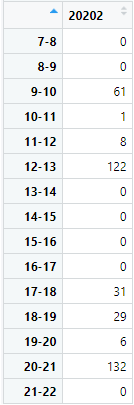
\includegraphics[scale = 0.8]{vec_alum_sim_EstadisticaIII} %width=\textwidth
\caption{\textit{Ejemplo de vector con demanda simulada para el 2020-2}}\label{vec_alum_sim}
\end{figure}

Obtuvimos vectores con la demanda simulada para cada una de las materias y formamos una matriz de $15 \times 333$. En la figura \ref{matDemandaAlum} podemos ver un ejemplo de cómo se ve la matriz formada.

Analicemos 2 pares de grupos, primero veamos la segunda y la quinta columna, que corresponden a las materias de \textit{Álgebra Superior II} y \textit{Geometría Analítica I}, respectivamente. Ambas son materias obligatorias para Actuaría, Matemáticas y Matemáticas Aplicadas. La primera corresponde a semestres pares y la segunda a semestres pares. Notamos que para \textit{Geometría Analítica I}, se tienen alumnos prácticamente en cada hora, pero el número no es muy grande, a diferencia de los alumnos simulados para \textit{Álgebra Superior II}, en donde hay varias horas con cero alumnos simulados pero hay dos grandes cantidades, una a las 9hrs con 832 alumnos y la otra a las 18hrs con 224 alumnos. Con esta comparación podemos ejemplificar la diferencia entre una materia que corresponde a semestres pares con una de semestres impares.

Ahora analicemos las columnas 4 y 8, correspondientes a las materias de \textit{Seminario de Topología A} y \textit{Probabilidad II}. La primera es una materia optativa para Matemáticas y la segunda es una materia obligatoria para Actuaría, correspondiente a semestres pares y optativa para Ciencias de la Computación, Matemáticas y Matemáticas Aplicadas. El número total de alumnos simulados para \textit{Seminario de Topología A} es menor a 20, en cambio para \textit{Probabilidad II} se tiene una gran cantidad de alumnos a las 8hrs, 9hrs y 10hrs. Considerando los valores que se tienen en el turno vespertino para \textit{Probabilidad II}, notamos que a las 19hrs también hay una gran cantidad de alumnos. Con esta comparación podemos ejemplificar la diferencia entre una materia obligatoria y una optativa, así como la diferencia entre el turno matutino y vespertino.


\begin{figure}[H]
\centering
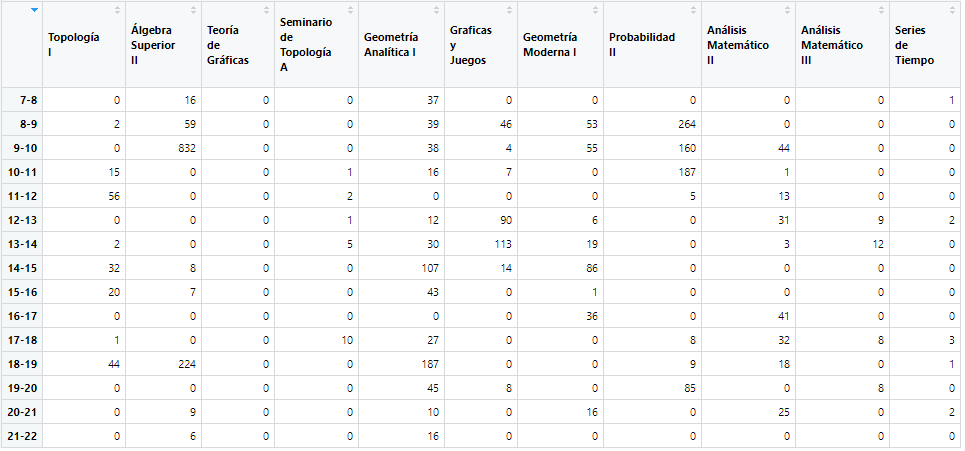
\includegraphics[scale = 0.7]{mat_demanda_alumnos} %width=\textwidth
\caption{\textit{Ejemplo de matriz con demanda simulada para el 2020-2}}\label{matDemandaAlum}
\end{figure}





\section{Simulación de tamaño de grupos}

En esta sección vamos a explicar cómo hicimos la simulación del tamaño de grupos. Vamos a definir al tamaño de un grupo como el número de alumnos que va a tener cada grupo.






\section{Obtención de información para solicitudes}

Antes de iniciar las simulaciones de elección de materia y de horario obtuvimos un vector y una matriz con la información de las materias y de los profesores, respectivamente.

En el caso de las materias, el vector \textit{vec\_nom\_materias\_total} lo obtuvimos a partir de la matriz \textit{m\_grande\_total} del semestre 2008-1 al 2020-1. No tiene nombres repetidos. Tiene 333 materias.

En el caso de los profesores, la matriz \textit{mat\_nom\_prof\_total} tiene 2 columnas. En la primer columna se tienen los nombres de todos los profesores que han impartido clase desde el semestre 2015-1 hasta el 2020-1. Dichos nombres los obtuvimos de la matriz \textit{m\_grande\_total} de los semestres correspondientes.

En la segunda columna de la matriz, se tiene un $1$ si el profesor es de tiempo completo y un $0$ si no. Para llenarla ingresamos a la página \url{http://www.matematicas.unam.mx/index.php/nosotros/profesores-de-tiempo-completo} del Departamento de Matemáticas. Con la aplicación \textit{SelectorGadget} seleccionamos el vector con el nombre de los profesores de tiempo completo. En la figura \ref{profTC_SelectorGadget} podemos ver el código CSS que utilizamos para obtener los datos en R. También observamos que se seleccionaron 94 profesores.

\begin{figure}[H]
\centering
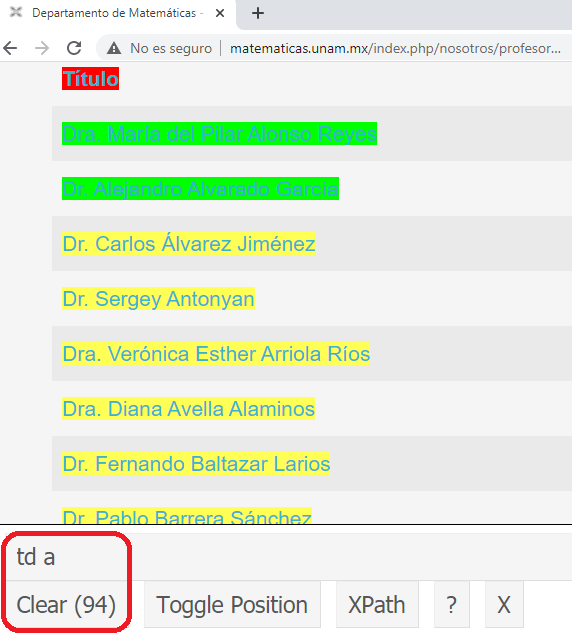
\includegraphics[scale = 0.8]{profesores_TC_SelectorGadget} %width=\textwidth
\caption{\textit{Profesores de tiempo completo: SelectorGadget}}\label{profTC_SelectorGadget}
\end{figure}

Al extraer la información en R obtuvimos un vector con 94 entradas. En la figura \ref{profTC_sinLimpiar} podemos ver los primeros 20 valores del vector. Notamos que cada entrada del vector inicia con los caracteres $\backslash n \backslash t \backslash t \backslash t \backslash t \backslash t \backslash t \backslash t$. Estos caracteres, en la presentación final de la página de internet, indican un salto de línea y las tabulaciones o espacios que se tienen de izquierda a derecha.

\begin{figure}[H]
\centering
\includegraphics[scale = 0.8]{profesores_TC_sinLimpiar} %width=\textwidth
\caption{\textit{Vector de profesores de tiempo completo}}\label{profTC_sinLimpiar}
\end{figure}

Limpiamos los datos para obtener un vector que sólo tuviera los nombres de los profesores. Eliminamos el título de cada uno porque en los horarios publicados en las páginas de la FC sus nombres no tienen título. También eliminamos los espacios finales que había en algunos nombres.

De esta manera obtuvimos el vector con el nombre de los profesores de tiempo completo del Departamento de Matemáticas. Dicho vector lo comparamos con la primer columna de la matriz \textit{mat\_nom\_prof\_total}, cuando los nombres coincidieron, pusimos un $1$ en el renglón correspondiente.

Al limpiar los datos encontramos 11 nombres que analizamos a mano porque no aparecía el $1$ en su respectivo renglón. Encontramos que no aparecía la información necesaria en la matriz \textit{mat\_nom\_prof\_total} por diferencias en los nombres. Encontramos diferencias por acentos, por mayúsculas y por nombre incompleto. En la tabla \ref{DifNomProfTC} vemos los nombres que aparecen en las páginas de FC comparados con los que aparecen en la página del Departamento de Matemáticas.

\begin{table}[h]
\centering
\resizebox{\textwidth}{!}{%
\begin{tabular}{|c|c|}
\hline 
\textbf{Nombre en páginas de FC} & \textbf{Nombre en página del Depto. de Matemáticas} \\ 
\hline 
Alejandro Ricardo Garciadiego Dantan & Alejandro Ricardo Garciadiego Dantán \\ 
\hline 
Edith Corina Sáenz Valadez & Edith Corina Sáenz Valadéz \\ 
\hline 
Emilio Esteban Lluis Puebla & Emilio Lluis Puebla \\
\hline 
Guillermo Javier Francisco Sienra Loera & Guillermo Sienra Loera \\
\hline 
María Asunción Begoña Fernández Fernández & Ma. Asunción Begoña Fernández Fernández \\ 
\hline 
María Concepción Ana Luisa Solís González-Cosío & Ana Luisa Solís González Cosío \\ 
\hline
María Isabel Puga Espinosa & Isabel Puga Espinosa \\ 
\hline 
María Lourdes Velasco Arreguí & María de Lourdes Velasco Arregui \\ 
\hline 
Mucuy-Kak del Carmen Guevara Aguirre & Mucuy-kak del Carmen Guevara Aguirre \\ 
\hline 
Oscar Alfredo Palmas Velasco & Óscar Alfredo Palmas Velasco \\ 
\hline 
Úrsula Xiomara Iturrarán Viveros & Úrsula Iturrarán Viveros \\ 
\hline 
\end{tabular}
} 
\caption{\textit{Diferencias en nombres de profesores de tiempo completo}}\label{DifNomProfTC}
\end{table}

Finalmente en la matriz \textit{mat\_nom\_prof\_total} se tiene la información de 1387 profesores de los cuales 94 son profesores de tiempo completo.

Algunas notas a considerar de esta matriz son:

\begin{itemize}
\item[-] Hay profesores que se repiten por diferencia de acentos. Ej. \textit{César Alejandro Arellano Ruíz, Luis Eduardo García Hernández}

\item[-] Hay profesores que se repiten por tener a lado el nombre de los ayudantes. Ej. \textit{Fermín Alberto Viniegra Heberlein, Edgar Vázquez Luis}

\item[-] Puede haber profesores que ya no impartan clases en la FC.
\end{itemize}


\section{Simulación de solicitudes de profesores oculta y pseudo-real}

En esta sección vamos a explicar cómo hicimos la simulación de la solicitud de los profesores. En la vida real los profesores pueden elegir libremente las materias que quieren impartir y seleccionan las horas a las que desean impartir sus clases. Dado que no contamos con esa información decidimos simular la elección de materias y horarios en base a la información que tenemos de semestres anteriores.

Como vimos en el diagrama \ref{DF_genAsig} simulamos dos veces las solicitudes de los profesores, en el proceso de asignación. A la primera vez que simulamos las solicitudes la llamaremos \textit{Solicitud oculta} y a la segunda la llamaremos \textit{Solicitud pseudo-real}. La explicación de su uso lo vemos a continuación.

\begin{itemize}
\item[-] Solicitud oculta: La llamamos oculta porque nos ayuda para la generación de los esqueletos. No influye directamente en la asignación final.

\item[-] Solicitud pseudo-real: Es la simulación de las posibles elecciones que los profesores harían en la vida real.
\end{itemize}




\subsection{Simulación de elección de materia}

\subsection{Simulación de elección de horario}



\section{Simulación de esqueletos}

Matriz de 2 columnas (Materia-Horario). En el renglón $i$ se tiene la información de cada grupo simulado para \textit{t+1}.

Se utiliza un matriz auxiliar de 3 columnas (Materia-Horario-Demanda\_Alum). En el renglón $i$ se tiene la información del número de alumnos simulados para la hora y materia correspondientes.

\begin{figure}[H]
\centering
\includegraphics[scale = 0.8]{Ej_esqueleto_20202} %width=\textwidth
\caption{\textit{Ejemplo de esqueleto para el semestre 2020-2}}\label{esqueleto20202}
\end{figure}

\section{Calificación de esqueletos de horario}

\begin{eqnarray*}
L_{materia} &=& -1 \,\,\,\,\,\,  \text{por cada materia no impartida}\\
x &=& \text{promedio}\\
y &=& \text{cupo}\\
L_{dif\_p\_c} (x,y) &=& \begin{cases}
    \dfrac{a}{190} (x-y)  & \quad \text{si } x<y\\
    - \dfrac{b}{190} (x-y)  & \quad \text{si } x\geqslant y
  \end{cases}\\
a &=& 0.5\\
b &=& 0.8\\
L_{categoria}^{1} (mat,solicitud) &=& -c(categoria - 1)\\
L_{categoria}^{2} (mat,solicitud) &=& -c_{1}(categoria)
\end{eqnarray*}

Al momento de simular las solicitudes de materias para los profesores suponemos que la que está en primer lugar es la materia que más quiere dar, en segundo lugar, la segunda que quiere dar.

Primero asignar grupos a los profesores de tiempo completo. Después asignar grupos faltantes a los profesores de asignatura.

$L_{materia}$ es la penalización por no tener en el esqueleto una materia que necesitamos.

$L_{dif\_p\_c}$ es la penalización en la asignación de salones. Se tiene un grupo de tamaño $x$ y un salón con capacidad $y$. Se penaliza con $\dfrac{a}{190}$ veces la diferencia entre $x$ y $y$ cuando el tamaño del grupo es menor a la capacidad del salón y se penaliza con $-\dfrac{b}{190}$ veces la diferencia entre $x$ y $y$ cuando el tamaño del grupo es mayor a la capacidad del salón.

El esqueleto depende de la demanda de alumnos y de las solicitudes de los profesores.

Primero se asignan materias a los profesores de tiempo completo y después a los de asignatura.

Los profesores de asignatura pueden quedarse sin materias asignadas.

Penalizaciones:

\begin{enumerate}
\item Si algún profesor pidió alguna materia y no se la dieron.

\item Si hay alumnos que necesitan una clase a alguna hora y no existe profesor que la imparta.

\item Con $\alpha \times num\_alumnos\_faltantes$ por cada alumno que te faltó en cada hora-materia que tenías que dar. $\alpha > 0$

\item Con $\beta \times num\_alumnos\_sobrantes$ por cada alumno que te pasaste en cada hora-materia que tenías que dar. $\beta > 0$

\end{enumerate}

Queremos el esqueleto con el menor valor en $\alpha + \beta$

Con esto se obtiene un nuevo esqueleto.


\section{Generación de asignaciones}

Matriz de 3 columnas (Materia-Horario-Profesor), la cual tiene la información de las asignaciones. A cada renglón de la matriz de esqueletos se agrega un profesor. Se genera con el esqueleto obtenido del proceso del AG y de las solicitudes de los profesores.

\subsection{Calificación de asignaciones de grupo}

%Los valores del modelo se muestran a continuación:

%\begin{lstlisting}[language=R, caption= \textit{Método Holt-Winters aditivo}]
%Holt-Winters' additive method 
%
%Call:
% hw(y = tsData, h = 1, seasonal = "additive", level = c(q1, q2)) 
%
%  Smoothing parameters:
%    alpha = 0.1247 
%    beta  = 1 
%    gamma = 1 
%
%  Initial states:
%    l = 111 
%    b = -22.5 
%    s = -50 50
%
%  sigma:  155.8648
%\end{lstlisting}

%\begin{figure}[H]
%\centering
%\includegraphics[scale = 0.8]{modelo_HW_total_alumnos_x_sem} %width=\textwidth
%\caption{\textit{Modelo del método aditivo de Holt-Winters: Total de alumnos por semestre}}
%\end{figure}




 %%4

\chapter{Algoritmo Genético}

El Algoritmo Genético (AG) es un método de computación evolutiva o \textit{machine learning}, basado en la teoría sintética de la evolución. Dicha teoría, a grandes rasgos, combina el mecanismo de la selección natural de Darwin con la genética de Mendel. Nos indica que el individuo más apto sobrevive, por lo que entre mejores sean los padres, mejor es la descendencia.

Actualmente el AG se utiliza para resolver problemas de búsqueda y optimización. Las áreas de aplicación son por ejemplo: economía, finanzas, medicina, ciencias sociales, investigación de operaciones, hidráulica, aeronáutica y química. Algunos ejemplos dentro de estas áreas son: diseño de redes de agua potable, optimización de portafolios de inversión, el problema del agente viajero y asignar asientos en un evento.

Los pasos del AG son los siguientes:

\begin{enumerate}
\item Selección: Se define una población de tamaño $n$. El valor de aptitud o adaptabilidad, de cada elemento en la población, se asigna al evaluar su utilidad en la función objetivo. Entre mejor sea el elemento, más alto será su valor de adaptabilidad. Se eligen 2 elementos de la población, llamados padres. La selección de los padres depende de qué tan aptos sean. Con dichos padres se va a formar un hijo.

\item Cruce: Con cierta probabilidad se toma información de los padres. Dicha información la llamaremos genes.

\item Mutación: Cada gen agregado al hijo tiene una probabilidad pequeña de mutar.

\item Reemplazamiento: Se repiten los 3 pasos anteriores hasta formar $n$ hijos y poder reemplazar la población.
\end{enumerate}

Con este proceso se obtiene una generación. El número de generaciones así como el tamaño de la población se fijan antes de iniciar con el algoritmo. En la \figurename{~\ref{fig_AG}} podemos ver el diagrama de los pasos mencionados.

\begin{figure}[H]
\centering
\includegraphics[scale = 0.8]{diagrama_flujo_AG} %width=\textwidth
\caption[\textit{Diagrama de flujo del Algoritmo Genético}]{\textit{Se muestra el diagrama de flujo que se sigue en el Algoritmo Genético.}}\label{fig_AG}
\end{figure}

En la siguiente sección explicaremos cómo encontramos una buena asignación utilizando el AG. Cabe mencionar que Reeves y Rowe en su libro \textit{Genetic Algorithms: Principles and Perspectives} [\ref{ReevesRowe}], nos indican que se puede generar una nueva población haciendo el cruce y la mutación o utilizando sólo una de ellas. En nuestro caso, la estrategia que seguimos fue utilizar ambas.


\section{Algoritmo Genético aplicado a los horarios} \label{Sec_AG_aplicado}

El objetivo principal de este proyecto es obtener una matriz con la asignación final de materias, profesores y horas. Para ello haremos uso del AG. A continuación vamos a definir los términos que utilizaremos:

\begin{itemize}
\item[-] Asignación: Matriz de 3 columnas con la información de materias, profesores y horarios.

\item[-] Población: Conjunto de $n$ asignaciones.

\item[-] Padre: Asignación seleccionada, de la población, para formar un hijo.

\item[-] Gen: Vector de 3 entradas (Materia, Profesor, Horario) con la información extraída de una asignación.

\item[-] Hijo: Asignación formada a partir de los genes de 2 padres.

\item[-] Probabilidad de mutación: Debe de ser un valor pequeño. %Definimos \textit{prob\_mutacion} $ = \dfrac{1}{24} \approx 0.04$

\item[-] Generación: Se tiene una generación cuando se han creado $n$  hijos y se puede reemplazar la población.
\end{itemize}

Los pasos que seguimos para obtener la asignación final son:

\begin{enumerate}
\setcounter{enumi}{-1}
\item \textbf{Crear un archivo \textit{xlsx}} \label{paso_cero}

Crear un archivo \textit{xlsx} con 3 hojas:

\begin{itemize}
\item[-] Horario: Contiene una asignación predefinida con los grupos que se desean tener en la asignación final.

\item[-] Materias: Contiene el nombre de las materias del vector \textit{vec\_nom\_materias} (ver Sección \ref{Sec_NomMaterias}).

\item[-] Profesores: Contiene la matriz \textit{mat\_nom\_prof}, con la información de cada profesor (ver Sección \ref{nomProfesores}).
\end{itemize}

Las hojas \textit{Materias} y \textit{Profesores} nos sirven de guía para llenar de manera adecuada la hoja \textit{Horario}. Evitando los problemas vistos en las secciones mencionadas de falta de acentos, nombres incompletos, entre otros.


\item \textbf{Definir parámetros iniciales}

\begin{itemize}
\item[-] $n \in \mathbb{N}$, tamaño de la población.

\item[-] $num\_generacion \in \mathbb{N}$, número de generaciones.

\item[-] $num\_max\_asig \in \mathbb{N}$, número máximo de materias que se le pueden asignar a un profesor.

\item[-] $prob\_mutar \in (0,0.05]$, probabilidad de mutación.
\end{itemize}

\item \textbf{Fijar semilla}

Con el comando \verb@set.seed(42)@ de \textit{R}, se fija la semilla para poder replicar las simulaciones. En este caso elegimos el 42.

\item \textbf{Simular esqueleto} \label{paso_sim_esq}

Obtener la matriz \textit{mat\_esqueleto} con el procedimiento visto en la Sección \ref{sec_esqueletos}.

\item \textbf{Simular solicitudes pseudo-reales} \label{paso_sim_solicitudes}

Obtener la matriz \textit{mat\_solicitudes} con el procedimiento visto en la Sección \ref{SimSolicitudesProfesores}.


\item \textbf{Leer archivo de excel}

Con la función \verb@read_excel()@, en \textit{R}, leer la hoja \textit{Horario} del archivo creado en el paso \ref{paso_cero}.

\item \textbf{Ajustar infomación en matrices}

Eliminar la información de las solicitudes correspondiente a la asignación predefinida. Se eliminan los grupos a esa hora o con esa materia.

Eliminar los grupos de la asignación predefinida en \textit{mat\_esqueleto}.


\item \textbf{Definir matrices auxiliares}

Estas matrices nos ayudan durante el proceso sin alterar las matrices originales.

Definir \textit{mat\_aux\_esqueleto} igual a \textit{mat\_esqueleto}.

Definir \textit{mat\_aux\_solicitudes} igual a \textit{mat\_solicitudes}.

%Estas matrices nos ayudan a eliminar información que ya no necesitamos durante el proceso sin alterar las matrices originales.


\item \textbf{Generar una población inicial}

Se generan $n$ asignaciones a partir del esqueleto simulado en el paso \ref{paso_sim_esq} y de las solicitudes pseudo-reales simuladas en el paso \ref{paso_sim_solicitudes}.

Para cada asignación, comparamos el número de solicitudes con el número de grupos simulados en el esqueleto. Ésto por materia y por hora. Se tienen dos casos:

\begin{enumerate}
\item[a)] El número de solicitudes es mayor al número de grupos simulados. En este caso se asignan los grupos tomados de una muestra aleatoria de las solicitudes. El tamaño de la muestra es igual al número de grupos simulados para la materia y hora correspondientes.

\item[b)] El número de solicitudes es menor o igual al número de grupos simulados. Se asignan todos los grupos en la solicitud, para la materia y hora correspondientes.
\end{enumerate}

De esta manera se asignan todos los posibles grupos que se hayan solicitado. Se debe de considerar lo siguiente:

\begin{itemize}
\item[-] Un profesor no puede impartir diferentes materias a la misma hora.

\item[-] Un profesor no puede impartir la misma materia en diferentes horarios.

\item[-] Un profesor no puede tener más de \textit{num\_max\_asig} materias asignadas.
\end{itemize}

\item \textbf{Calificar cada asignación de la población} \label{paso_califica_asig}

Cada asignación tiene 2 tipos de calificaciones:

\begin{enumerate}
\item Por gen: Se califica cada gen de la asignación. Se premia con +5 si el profesor asignado es de tiempo completo. Se penaliza con -1 por cada asignación que pudo haber tenido un profesor de tiempo completo y tiene un profesor de asignatura. Para tener una calificación diferente para cada grupo, sumamos a cada gen una $\epsilon \in [0,0.1]$.

\item Global: Se califica la asignación completa. Se penaliza por cada grupo en el esqueleto sin profesor, se resta de acuerdo a la diferencia relativa. Se penaliza con -10 por cada materia pedida por algún profesor de tiempo completo y no se le asignó. Se suma el promedio de las calificaciones por gen.

Nota:
Si el número máximo de asignaciones es 2 y un profesor pidió 3 o más  materias pero sólo se le asignó 1, entonces se penaliza una materia. Si se le asignaron, 2 no hay penalización.
\end{enumerate}

\item \textbf{Ordenar de acuerdo a la calificación}

Los genes de cada asignación y las asignaciones se ordenan de menor a mayor calificación.

\item \textbf{Elegir 2 padres} \label{paso_elegir_padres}

Los padres se eligen con probabilidad: $\mathbb{P}(\text{elegir la asignación } i \text{ ya ordenada}) = \dfrac{2i}{n(n+1)}$, donde $i$ es la posición de la asignación con respecto a su calificación. Se desea elegir con mayor probabilidad las asignaciones con mejor calificación.

\item \textbf{Elegir un gen} \label{paso_elegir_gen}

Primero se elige al azar un padre (ambos tienen probabilidad $0.5)$. Una vez que se eligió un padre, seleccionar un gen: $\mathbb{P}(\text{elegir el gen } i \text{ ya ordenado}) = \dfrac{2i}{g(g+1)}$, donde $i$ es la posición del gen en la asignación con respecto a su calificación y $g$ es el número de genes que tiene la asignación. Se quiere elegir con mayor probabilidad los genes con mejor calificación.

\item \textbf{Mutación}

Se simula un número aleatorio, si ese número es menor a la probabilidad de mutación, entonces el gen tiene una mutación. Si un gen muta, se elige un gen de las solicitudes pseudo-reales y se intercambia por el gen previamente seleccionado.

\item \textbf{Agregar gen}

Una vez seleccionado el gen, éste se agrega al hijo.

\item \textbf{Ajustar información} \label{paso_ajusta_info}

\begin{itemize}
\item[a)] Disminuir en 1 al grupo correspondiente al gen en \textit{mat\_aux\_esqueleto}.

\item[b)] Quitar la información a los padres, del profesor en el gen elegido:

\begin{itemize}
\item[-] A esa hora y con esa materia para evitar que se elijan genes repetidos para el hijo. Esto puede ocurrir por ejemplo cuando ambos padres tienen el mismo gen.

\item[-] A esa hora porque los profesores no pueden impartir más de una clase a la misma hora.

\item[-] Con esa materia porque no se les puede asignar la misma materia en diferentes horarios.

\item[-] Cualquier materia a cualquier hora cuando el profesor ya tiene el número máximo de materias asignadas.
\end{itemize}

\item[c)] Quitar la información correspondiente en la matriz \textit{mat\_aux\_solicitudes}.
\end{itemize}

\item \textbf{Repetir \ref{paso_elegir_gen} - \ref{paso_ajusta_info}}

Repetir los pasos \ref{paso_elegir_gen} al \ref{paso_ajusta_info} hasta que uno de los padres se quede sin genes.

\item \textbf{Añadir genes} \label{paso_agrega_genes}

Agregar al hijo los genes del padre que aún tiene información.

Con el algoritmo utilizado en la generación de la población inicial, agregar los grupos que falta por asignar de \textit{mat\_aux\_esqueleto}. Ésto tomando en cuenta las solicitudes en \textit{mat\_aux\_solicitudes}.

\item \textbf{Repetir \ref{paso_elegir_padres} - \ref{paso_agrega_genes}}

Repetir los pasos \ref{paso_elegir_padres} al \ref{paso_agrega_genes} $n$ veces para poder formar una generación.

\item \textbf{Reemplazar población} \label{paso_reemplaza_pob}

Reemplazar a la población con la que se formó la generación.

\item \textbf{Repetir \ref{paso_califica_asig} - \ref{paso_reemplaza_pob}}

Repetir los pasos \ref{paso_califica_asig} al \ref{paso_reemplaza_pob} hasta completar el número de generaciones deseadas.

\item \textbf{Asignación final}

Definir la asignación final como el hijo mejor calificado de la última generación.

\item \textbf{Agregar grupos predefinidos}

Agregar los grupos de la asignación predefinida a los grupos de la asignación final.
\end{enumerate}


Algunas notas que se deben de considerar en la asignación final:

\begin{itemize}
\item[-] Algunos profesores se les asignaron 2 cálculos.

\item[-] Puede haber profesores que ya no imparten clases en la Facultad.

\item[-] No se asignaron todos los grupos simulados en el esqueleto. Ésto porque:

\begin{itemize}
\item[a)] No hay solicitudes de esas materias a esas horas.

\item[b)] Se asignaron otras materias a los profesores en esas horas.
\end{itemize}

\item[-] Es posible que la asignación final no sea la mejor calificada de todas las generaciones.
\end{itemize}


\section{Resultados del Algoritmo Genético}

Hicimos algunas pruebas con el AG para definir los parámetros de la asignación final. En la \tablename{~\ref{ResumenPruebasAG}} se puede ver un resumen con los resultados de dichas pruebas. A continuación explicamos lo que contienen sus columnas.

\begin{itemize}
\item[(1)] Número de generaciones, para cada prueba.

\item[(2)] Tamaño de la población, para cada generación.

\item[(3)] Calificación del mejor elemento de todas las generaciones.

\item[(4)] Número de genes de la asignación final.

\item[(5)] Calificación de la asignación final de cada prueba.
\end{itemize}

En las últimas 2 pruebas la asignación final no tuvo la mejor calificación de todas las asignaciones generadas. Ésto puede ocurrir porque el AG explora diferentes posibilidades y no necesariamente son siempre mejores que las anteriores.

%También podemos observar que las calificaciones de los mejores elementos es cada vez mayor en cada prueba. Con ello podemos concluir que al incrementar el tamaño de la población o el número de generaciones la asignación final será cada vez mejor.
Al observar la última columna notamos que al incrementar el tamaño de la población o el número de generaciones la calificación de la asignación final es cada vez mejor. Si comparamos la prueba $1$ con la $2$ vemos que hay una diferencia de $11.82$ puntos, en la calificación. Se incrementaron 10 elementos a la población de 5 a 15 elementos.

Si ahora comparamos la prueba $1$ con la $3$ notamos que la diferencia es de $65.24$ puntos, en la calificación. En este caso se incrementó el número de generaciones de 3 a 6.

Con estas observaciones concluímos que hay un mayor incremento en la calificación cuando se aumenta el número de generaciones que el tamaño de la población.

\begin{table}[H]
\centering
\begin{tabular}{|c|c|c|c|c|}
\hline 
 \textbf{Generaciones} & \textbf{Población} & \textbf{Mejor calif.} & \textbf{Genes asig. final} & \textbf{Calif. asig. final} \\ \hline
 3 & 5 & -599.43 & 677 & -599.43 \\ \hline
 3 & 15 & -587.61 & 672 & -587.61 \\ \hline
 6 & 5 & -534.19 & 679 & -534.19 \\ \hline
 6 & 10 & -527.56 & 694 & -527.56 \\ \hline
 8 & 8 & -510.52 & 682 & -510.52 \\ \hline
 10 & 5 & -521.78 & 683 & -530.79 \\ \hline
 10 & 10 & -514.41 & 682 & -515.85 \\ \hline
\end{tabular}
\caption[\textit{Resumen de las pruebas del Algoritmo Genético}]{\textit{Se muestran los datos de las pruebas del Algoritmo Genético. Se observa una mejora en la calificación cuando se incrementa el número de generaciones o el tamaño de la población.}}\label{ResumenPruebasAG}
\end{table}

%> xtable(mat_info_AG)
%% latex table generated in R 4.0.2 by xtable 1.8-4 package
%% Sun Jan 10 17:34:18 2021
%\begin{table}[ht]
%\centering
%\begin{tabular}{rrrrrrrrr}
%  \hline
% & Num\_generaciones & Tam\_pob & Tiempo & Mejor\_calif & Num\_genes\_asig\_fin & Calif\_asig\_fin & Prom\_genes\_gen1 & Prom\_genes\_generaciones \\ 
%  \hline
%1 & 3.00 & 5.00 & 39.52 & -599.43 & 677.00 & -599.43 & 658.40 & 670.50 \\ 
%  2 & 3.00 & 15.00 & 116.99 & -587.61 & 672.00 & -587.61 & 659.20 & 672.50 \\ 
%  3 & 6.00 & 5.00 & 96.63 & -534.19 & 679.00 & -534.19 & 660.20 & 675.00 \\ 
%  4 & 6.00 & 10.00 & 176.08 & -527.56 & 694.00 & -527.56 & 658.70 & 675.64 \\ 
%  5 & 10.00 & 5.00 & 156.97 & -521.78 & 683.00 & -530.79 & 654.00 & 675.20 \\ 
%  6 & 10.00 & 10.00 & 394.80 & -514.41 & 682.00 & -515.85 & 658.40 & 678.24 \\ 
%   \hline
%\end{tabular}
%\end{table}


A continuación presentaremos los resultados obtenidos con el AG correspondientes a la prueba con 8 generaciones y 8 elementos por cada población. En esta prueba obtuvimos la mejor calificación en la asignación final de todas las pruebas realizadas. El número de genes varía dependiendo de cada asignación, en este caso se encuentra entre 650 y 690.


En la \figurename{~\ref{EjcalifMejoresHijos}} vemos las calificaciones de la mejor asignación por generación. Observamos que la mejora en la calificación es considerable de la población inicial a la segunda generación. Este fenómeno es común en el AG porque la primera generación se simula de manera aleatoria. Para la segunda generación es más probable elegir los mejores elementos de la población. Incluso a nivel gen se tiene una mayor probabilidad de elegir los mejores. Es por ello que se da esa gran diferencia en las calificaciones entre la generación 1 y la 2.

Notamos que la calificación del mejor elemento de la generación 6 es menor a la calificación de la generación 5. Con ésto podemos observar que las diferentes posibilidades que explora el AG no necesariamente son siempre mejores que las anteriores.


%\begin{figure}[H]
%\centering
%\includegraphics[scale = 0.7]{calif_mejores_hijos_g08_n08_m004_U510.pdf} %width=\textwidth
%\caption[\textit{Calificaciones de las mejores asignaciones por generación}]{\textit{Se muestran las calificaciones de la mejor asignación por generación. Se observa una mejora considerable en la calificación de la generación 1 a la 2.}}\label{EjcalifMejoresHijos}
%\end{figure}

En la \figurename{~\ref{boxplot_calif_x_generacion}} observamos las gráficas de caja de las calificaciones de las asignaciones, para cada generación. Hay una mejora considerable en las calificaciones de la generación 1 a la 2. Los puntos representan las calificaciones de cada asignación por generación. Notamos que las calificaciones de las asignaciones en la generación 6, son muy parecidas. A diferencia de las calificaciones en la generación 3, las cuales varían más.

%\begin{figure}[H]
%\centering
%\includegraphics[scale = 0.7]{boxplot_calif_g08_n08_m004_U510.pdf} %width=\textwidth
%\caption[\textit{Gráficas de caja de calificaciones de asignaciones por generación}]{\textit{Se muestran las gráficas de caja de las calificaciones de las asignaciones por generación. Se observa una mejora considerable en la calificación de la generación 1 a la 2.}}\label{boxplot_calif_x_generacion}
%\end{figure}

En la \figurename{~\ref{media_calif_x_generacion}} se puede ver el promedio de las calificaciones de las asignaciones por generación. Al igual que en las Figuras \ref{EjcalifMejoresHijos} y \ref{boxplot_calif_x_generacion} se observa una mejora considerable en la calificación de la generación 1 a la 2. Podemos observar que el promedio de las calificaciones de la generación 7 es menor que el promedio de las calificaciones de la generación 6.


%\begin{figure}[H]
%\centering
%\includegraphics[scale = 0.7]{media_calif_g08_n08_m004_U510.pdf} %width=\textwidth
%\caption[\textit{Media de calificaciones de asignaciones por generación}]{\textit{Se muestra el promedio de las calificaciones de las asignaciones por generación. Se observa una mejora considerable en la calificación de la generación 1 a la 2.}}\label{media_calif_x_generacion}
%\end{figure}

En la \figurename{~\ref{var_calif_x_generacion}} se ve la varianza de las calificaciones de las asignaciones por generación. El valor más pequeño se observa en la generación 6. Al ver la \figurename{~\ref{boxplot_calif_x_generacion}} en dicha generación, notamos que los puntos tienen valores muy similares. La varianza más grande se obtiene en la generación 3. Ésto también se puede ver en la \figurename{~\ref{boxplot_calif_x_generacion}}.


\begin{figure}[H]
\centering
\includegraphics[scale = 0.67]{calif_mejores_hijos_g08_n08_m004_U510.pdf} %width=\textwidth
\caption[\textit{Calificaciones de las mejores asignaciones por generación}]{\textit{Se muestran las calificaciones de la mejor asignación por generación. Se observa una mejora considerable en la calificación de la generación 1 a la 2.}}\label{EjcalifMejoresHijos}
\end{figure}


\begin{figure}[H]
\centering
\includegraphics[scale = 0.67]{boxplot_calif_g08_n08_m004_U510.pdf} %width=\textwidth
\caption[\textit{Gráficas de caja de calificaciones de asignaciones por generación}]{\textit{Se muestran las gráficas de caja de las calificaciones de las asignaciones por generación. Se observa una mejora considerable en la calificación de la generación 1 a la 2.}}\label{boxplot_calif_x_generacion}
\end{figure}

\begin{figure}[H]
\centering
\includegraphics[scale = 0.67]{media_calif_g08_n08_m004_U510.pdf} %width=\textwidth
\caption[\textit{Media de calificaciones de asignaciones por generación}]{\textit{Se muestra el promedio de las calificaciones de las asignaciones por generación. Se observa una mejora considerable en la calificación de la generación 1 a la 2.}}\label{media_calif_x_generacion}
\end{figure}


\begin{figure}[H]
\centering
\includegraphics[scale = 0.67]{varianza_g08_n08_m004_U510.pdf} %width=\textwidth
\caption[\textit{Varianza de calificaciones de asignaciones por generación}]{\textit{Se muestra la varianza de las calificaciones de las asignaciones por generación. Se observa una disminución considerable de la generación 5 a la 6. El valor más grande se encuentra en la generación 3.}}\label{var_calif_x_generacion}
\end{figure}

En la \figurename{~\ref{boxplot_num_genes_x_generacion}} podemos ver las gráficas de caja del número de genes en las asignaciones por generación. Los puntos representan el número de genes de cada asignación por generación. Notamos que la media de la generación 2 es considerablemente mayor que la media de la generación 1.

De la generación 1 a la 6 los promedios del número de genes tienden a ser cada vez mayores. Ésto se logra al agregar los grupos que aún se pueden asignar después de hacer el cruce con los padres.

También podemos observar que el promedio del número de genes en las generaciones 7 y 8 es menor al promedio del número de genes en la generación 6. En las generaciones 4 y 7, el número de genes varía mucho.

\begin{figure}[h]
\centering
\includegraphics[scale = 0.7]{boxplot_num_genes_g08_n08_m004_U510.pdf} %width=\textwidth
\caption[\textit{Gráficas de caja del número de genes en asignaciones por generación}]{\textit{Se muestran las gráficas de caja del número de genes en asignaciones por generación. Se observa que los valores tienen una tendencia no decreciente.}}\label{boxplot_num_genes_x_generacion}
\end{figure}

%****************************************************************************

%En un esqueleto simulado para el 2020-2 se tuvieron 1018 grupos. De éstos se asignaron 612. Encontramos que 262 grupos sin asignación correspondían a materias optativas. Prácticamente $\dfrac{1}{4}$ de los grupos no asignados son de materias optativas. Ésto se debe a que se pueden asignar \textit{num\_max\_asig} materias obligatorias a los profesores por lo que ya no se les asignan las optativas. En la matriz de solicitudes puede haber grupos que no están en la asignación final. Ésto por el cruce de los padres.
%
%\begin{eqnarray*}
%\dfrac{612}{1018} &=& 60.11\% \text{grupos asignados}\\
%\dfrac{262}{1018} &=& 25.73\% \text{grupos de optativas sin asignación}\\
%\dfrac{1018 - (612 + 262)}{1018} &=& \dfrac{144}{1018} = 14.14\% \text{grupos de obligatorias sin asignación}
%\end{eqnarray*}

%\begin{figure}[H]
%\centering
%\includegraphics[width=\textwidth]{num_genes_generaciones_1_2} %scale = 0.7
%\caption[\textit{Número de genes en generaciones 1 y 2}]{\textit{Número de genes en generaciones 1 y 2}}
%\end{figure}

%Sabemos que la asignación final es el mejor elemento de la última generación. En la \tablename{~\ref{submatAsigFinal}} presentamos una submatriz de la asignación final. Cabe aclarar que los datos se ordenaron con respecto a la materia (en orden alfabético) y por hora (de menor a mayor). La matriz completa se puede ver el el Apéndice \ref{Ej_AsigFinal}. Dicha matriz tiene 630 grupos asignados, cada uno con materia, profesor y horario correspondiente. En el semestre 2020-1 se tuvieron 747 grupos reales. Se simularon 1011 grupos en \textit{mat\_esqueleto}. Las materias optativas y obligatorias de los siguientes porcentajes se consideran con respecto a la carrera de Actuaría.
%
%\begin{eqnarray*}
%\dfrac{630}{1011} &=& 62.31\% \text{grupos asignados}\\
%\dfrac{229}{1011} &=& 22.65\% \text{grupos de optativas sin asignación}\\
%\dfrac{17}{1011} &=& 1.68\% \text{grupos de inglés sin asignación}\\
%\dfrac{1011 - (630 + 229 + 17)}{1011} &=& \dfrac{135}{1011} = 13.35\% \text{grupos de obligatorias sin asignación}\\
%\dfrac{630}{747} &=& 84.33\% \text{grupos asignados comparado con el 2020-1}
%\end{eqnarray*}

Sabemos que la asignación final es el mejor elemento de la última generación. En la \tablename{~\ref{submatAsigFinal}} presentamos una submatriz de una asignación final. Cabe aclarar que los datos se ordenaron con respecto a la materia (en orden alfabético) y por hora (de menor a mayor). La matriz completa se puede ver en el Apéndice \ref{Ej_AsigFinal}.

Dicha matriz tiene 682 grupos asignados, cada uno con materia, profesor y horario correspondiente. En el semestre 2020-1 se tuvieron 747 grupos reales. Se simularon 1091 grupos en \textit{mat\_esqueleto} para el semestre 2020-2.

\begin{table}[H]
\centering
\begin{tabular}{|c|p{7cm}|p{4.7cm}|c|}
\hline
\textbf{ } & \textbf{Materia} & \textbf{Profesor} & \textbf{Horario} \\ \hline
1 & Administración Actuarial del Riesgo & Fernando Pérez Márquez & 7 \\ \hline
  133 & Cálculo Diferencial e Integral I & Elena de Oteyza de Oteyza & 7 \\ \hline
  156 & Cálculo Diferencial e Integral II & Héctor Méndez Lango & 11 \\ \hline
%  353 & Inferencia Estadística & Martha Angélica Montes Fonseca & 18 \\ \hline
  401 & Manejo de Datos & José Alfredo Cobián Campos & 13 \\ \hline
  418 & Matemáticas Financieras & Irma Rocío Zavala Sierra & 7 \\ \hline
  498 & Modelos de Supervivencia y de Series de Tiempo & Margarita Elvira Chávez Cano & 10 \\ \hline
%  505 & Modelos no Paramétricos y de Regresión & Jaime Vázquez Alamilla & 8 \\ \hline
  510 & Modelos no Paramétricos y de Regresión & Lizbeth Naranjo Albarrán & 11 \\ \hline
  534 & Probabilidad I & María Asunción Begoña Fernández Fernández & 10 \\ \hline
  539 & Probabilidad II & Daniel Alejandro Zurita Gutiérrez & 8 \\ \hline
  561 & Procesos Estocásticos I & Arrigo Coen Coria & 10 \\ \hline
  567 & Productos Financieros Derivados & Jesús Agustín Cano Garcés & 10 \\ \hline
%  679 & Variable Compleja I & Micho Durdevich Lucic & 16 \\ \hline
%  680 & Variable Compleja I & Mico Djurdjevic & 16 \\ \hline
  682 & Variable Compleja I & Jesús Manuel Mayorquín García & 19 \\ \hline
\end{tabular}
\caption[\textit{Submatriz con asignación final}]{\textit{Se muestra una submatriz de la asignación final. Cada renglón tiene la información de un grupo con una materia, profesor y horario asignado.}}\label{submatAsigFinal}
\end{table}


A continuación presentamos algunos porcentajes que nos permiten hacer diferentes comparaciones. Las materias optativas y obligatorias que se mecionan, se consideran con respecto a la carrera de Actuaría.

\begin{eqnarray*}
\dfrac{682}{1091} &=& 62.51\% \text{ grupos asignados}\\\\
\dfrac{409}{1091} &=& 37.48\% \text{ grupos no asignados}\\\\
\dfrac{241 + 18}{1091} &=& 23.73\% \text{ grupos de optativas e inglés sin asignación}\\\\
%\dfrac{18}{1091} &=& 1.64\% \text{ grupos de inglés sin asignación}\\\\
\dfrac{150}{1091} &=& 13.74\% \text{ grupos de obligatorias sin asignación}\\\\ %\dfrac{1091 - (682 + 241 + 18)}{1091}
\dfrac{682}{747} &=& 91.29\% \text{ grupos asignados comparados con el 2020-1}
%\dfrac{1091}{747} &=& 146.05\% \text{ grupos simulados para 2020-2 comparados con el 2020-1}
\end{eqnarray*}

%\begin{figure}[H]
%\centering
%\includegraphics[width=\textwidth]{dif_rel_optativas_sin_gpo} %scale = 0.7
%\caption[\textit{Optativas sin grupos asignados}]{\textit{Optativas sin grupos asignados}}
%\end{figure}

Notamos que casi una cuarta parte de los grupos simulados en \textit{mat\_esqueleto} corresponde a materias optativas y de inglés sin asignación. Ésto ocurre por dos principales motivos:

\begin{enumerate}
\item No hay solicitudes en \textit{mat\_solicitudes} de los grupos no asignados. Existen materias optativas que no se imparten todos los semestres. Por ello hay ocasiones en las que no se simula la solicitud.

\item Se les asigna otra materia a esa hora a los profesores que hayan solicitado alguna optativa. Usualmente se les asigna una obligatoria a la hora en la que solicitaron la optativa.
\end{enumerate}

La principal razón por la que se tiene alrededor de un $10\%$ de materias obligatorias sin asignar es por la forma en la que definimos \textit{mat\_esqueleto}. El modelo de mezcla de normales nos permite que los grupos se distribuyan a lo largo de las horas sin tener picos demasiado altos.

Ésto se basa en el supuesto de que los alumnos tienen la misma preferencia por una materia a cierta hora, o a la hora anterior o a la siguiente. Es decir, si un alumno elige \textit{Probabilidad I} a las 10hrs, le es indistinto si la toma a las 9hrs, a las 10hrs o a las 11hrs.

Este fenómeno se observa con mayor claridad en las materias con horarios muy específicos como \textit{Teoría del Seguro, Matemáticas Actuariales para Seguro de Daños, Fianzas y Reaseguro} o \textit{Matemáticas Actuariales del Seguro de Personas I}.

En el caso de \textit{Teoría del Seguro} se simularon 4 grupos en \textit{mat\_esqueleto}, a las 8hrs, 10hrs, 13hrs y 19hrs. Las solicitudes simuladas se pueden ver en la \figurename{~\ref{sol_TeoSeguro}}. Notamos que sólo hay solicitudes a las 8hrs y a las 19hrs. Con estos datos el algoritmo sólo puede asignar dos grupos, uno a las 8hrs y otro a las 19hrs.

\begin{figure}[H]
\centering
\includegraphics[scale = 0.8]{solicitudes_teoria_del_seguro} %width=\textwidth
\caption[\textit{Solicitudes simuladas de la materia ``Teoría del Seguro'' para el semestre 2020-2}]{\textit{Se muestran las solicitudes simuladas de la materia ``Teoría del Seguro'' para el semestre 2020-2.}}\label{sol_TeoSeguro}
\end{figure}

Por estas razones el algoritmo asigna alrededor del $60\%$ de los grupos simulados. Para aumentar este porcentaje, se pueden definir manualmente grupos de materias optativas o de inglés. Ésto en el archivo de excel definido en el paso \ref{paso_cero} del algoritmo. Dado que se elimina la información en las solicitudes antes de realizar el AG, no se tienen grupos repetidos en la asignación final.

 %%5

\chapter{Resultados del Algoritmo Genético}

En este capítulo presentamos la matriz con la asignación final después de haber aplicado el AG. Se simularon $g$ generaciones y el tamaño de la población es de \textit{tam\_poblacion}. Una vez terminado el proceso se extrajo el mejor elemento de la última generación. Éste elemento es la matriz que presentamos a continuación. Cabe aclarar que los datos se ordenaron con respecto a la materia (en orden alfabético) y por hora (de menor a mayor).

\dfNmatAsigFinal %%6

\chapter{Comportamiento de la selección}
 %%7

\chapter{Conclusiones}

\begin{enumerate}
\item Se encontró que el Algoritmo Genético es una buena opción para solucionar este problema de maximización. El problema de asignación de horarios se considera como un problema NP-duro. Por lo tanto se requiere un tiempo exponencial para encontrar la solución óptima. El Algoritmo Genético nos permite encontrar una buena solución en un periodo corto de tiempo. En la Sección \ref{Sec_Resultados_AG} se mostraron los resultados de una prueba con 8 generaciones y tamaño de población 8. El tiempo total para generar una asignación con dichos parámetros es apróximadamente 3.5 horas. Con ello se puede ayudar a agilizar la asignación de horarios actual.%no se puede resolver en un tiempo polinomial (razonable)

\item Este trabajo apoya las necesidades, con respecto a los horarios de las materias, de los alumnos de la Facultad de Ciencias. El número de grupos necesarios para el siguiente semestre se estima en base a la demanda del número de alumnos. Ésto nos permite proponer una asignación que depende del número de alumnos esperados en el siguiente semestre.

\item La división que se hizo de los datos es estadísticamente adecuada. En la Sección \ref{SimDemandaAlumnos} vemos que los datos están divididos por semestres pares e impares y por hora. El modelo distingue entre el tipo de semestre. Puede predecir el número de alumnos para un semestre par o impar. Al hacer la predicción por hora, se puede observar el comportamiento del turno matutino y el del turno vespertino.

\item Con el modelo de mezcla de normales es posible suavizar la distribución que tiene el tamaño de grupos por hora, como vimos en la Sección \ref{sec_esqueletos}. Ésto se basa en el supuesto de que los alumnos tienen la misma preferencia por una materia a cierta hora, o a la hora anterior o a la siguiente. %Es decir, si un alumno elige una materia a las 11hrs, le es indistinto si la toma a las 10hrs, a las 11hrs o a las 12hrs.

\item El poder definir grupos por medio de un archivo \textit{.xlsx} (ver Sección \ref{Sec_AG_aplicado}), otorga a los usuarios de este programa mayor control en las asignaciones. Con esto permitimos al usuario introducir parámetros iniciales que sean requeridos.

\item El algoritmo propuesto puede ser aplicado en otras escuelas o facultades que cuenten con características similares de información a las de la Facultad de Ciencias. También puede ser utilizado para resolver problemas generales de asignación de recursos.

\item En particular, para las carreras de la Facultad de Ciencias que no pertenecen al Departamento de Matemáticas, el programa realizado se puede ajustar. Algunas extensiones pueden ser: %Se debe de considerar lo siguiente: %(cada inciso tiene un ejemplo):

%\begin{itemize}
%\item[a)] Las materias impartidas en los laboratorios duran 2 o más horas: \url{http://www.fciencias.unam.mx/docencia/horarios/20191/1081/830}.
%
%\item[b)] No todas las materias se imparten todos los días: \url{http://www.fciencias.unam.mx/docencia/horarios/20192/1439/1419}.
%
%\item[c)] Existen materias que no duran horas enteras: \url{http://www.fciencias.unam.mx/docencia/horarios/20192/1081/104}.
%
%\item[d)] Hay materias que no inician en horas enteras: \url{http://www.fciencias.unam.mx/docencia/horarios/20172/181/1601}.
%\end{itemize}

\begin{itemize}
\item[-] Las materias impartidas en los laboratorios duran 2 o más horas.

\item[-] No todas las materias se imparten todos los días.

\item[-] Existen materias que no duran horas enteras.

\item[-] Hay materias que no inician en horas enteras.
\end{itemize}

\item La aplicación \textit{SelectorGadget} de \textit{Google} es útil para automatizar el proceso de la descarga de información en páginas web. Como vimos en la Sección \ref{Sec_ED_estructura_URL}, el número de páginas de las que sacamos la información es grande. El proceso de automatización nos sirvió para extraer información en poco tiempo. Este proceso se puede aplicar a diversos problemas. %No sólo para las páginas de la Facultad de Ciencias.

\end{enumerate}

 %%8

%%%%% Apéndices %%%%%
\backmatter %%Los "Capítulos" ya no se registran como tal en el índice general

%%%%%%%%%% A partir de aquí los apéndices se declaran como secciones, ya que el Capítulo es "Apéndices": %%%%%%%%%%

\begin{appendices}
\chapter{Materias agrupadas}\label{materias_agrupadas}

Vemos las materias que se actualizaron o cambiaron de nombre. Las negritas son los nombres y número de materia que tenían cuando el vector tenía 335 materias.


  \begin{itemize}
  \item Administración \textbf{(1)} -> Administración Actuarial (148) -> \textbf{Administración Actuarial del Riesgo} (288)
  
  \item Seminario de Inteligencia Artificial \textbf{(3)} -> \textbf{Recuperación y Búsqueda de Información en Textos} (257)
  
  \item \textbf{Seminario de Aplicaciones a las Ciencias Sociales y Administrativas (4)} -> Administración de Empresas de Software (258) -> Riesgo Tecnológico (278) -> Temas Selectos de Ingeniería de Software A (192)
  
  \item Probabilidad y Estadística \textbf{(5)} -> \textbf{Probabilidad I} (60)

\item \textbf{Mecánica Vectorial (6)} -> Cálculo Tensorial (248)

  
  \item Matemáticas Avanzadas de la Física \textbf{(12)} -> \textbf{Funciones Especiales y Transformadas Integrales} (53) -> Análisis de Fourier I (208) -> Análisis de Fourier II (231) -> Introducción a las Funciones Recursivas y Computabilidad (224)

  \item \textbf{Mecánica Analítica (13)} -> Introducción Matemática a la Mecánica Celeste (119)

  \item \textbf{Física Computacional (15)} -> Supercómputo (195)

  \item \textbf{Teoría de Gráficas (33)} -> Teoría de las Gráficas II (147)
  
  \item Graficas y Juegos \textbf{(36)} -> \textbf{Introducción a las Matemáticas Discretas} (311)
  
  \item Estadística I \textbf{(41)} -> \textbf{Inferencia Estadística} (300)
  
  \item Análisis de Redes \textbf{(44)} -> \textbf{Teoría de Redes} (152)
  
  \item Bases de Datos \textbf{(50)} -> Formación Científica I (330) -> Sistemas Manejadores de Bases de Datos (106) -> Sistemas de Bases de Datos (123) -> Grandes Bases de Datos (169) -> Fundamentos de Bases de Datos (241) -> Almacenes y Minería de Datos (269) -> \textbf{Manejo de Datos} (301) -> Programación II (51)
  
  \item \textbf{Análisis Numérico (54)} -> Análisis Numérico II (161) -> Temas Selectos de Análisis Numérico (321)
  
  \item \textbf{Seminario sobre Enseñanza de las Matemáticas I (56)} -> Seminario de Filosofía de la Ciencia I (118) -> Didáctica de las Matemáticas (319)
  
  \item Estadística II \textbf{(59)} -> \textbf{Modelos no Paramétricos y de Regresión} (284) -> Análisis de Regresión (113)
  
  \item Teoría de la Computación \textbf{(67)} -> \textbf{Autómatas y Lenguajes Formales} (240)
  
  \item Matemáticas Discretas \textbf{(68)} -> \textbf{Estructuras Discretas} (220)
  
  \item Programación I \textbf{(69)} -> \textbf{Programación} (287)
  
  \item \textbf{Procesos Estocásticos I (70)} -> Procesos Estocásticos (159)

  \item \textbf{Seminario de Geometría A (73)} -> Álgebra Geométrica (207) -> Geometría Algebraica II (209)
  
  \item Fianzas \textbf{(78)} -> Matemáticas Actuariales del Seguro de Daños (79) -> \textbf{Matemáticas Actuariales para Seguro de Daños, Fianzas y Reaseguro} (SN) -> Matemáticas Actuariales para Seguro de Daños (297) -> Reaseguro (98) -> Reaseguro Financiero (127)
  
  \item Teoría de Juegos I (143) -> \textbf{Teoría de Juegos en Economía (80)}

  \item Finanzas II \textbf{(82)} -> \textbf{Métodos Cuantitativos en Finanzas} (298)
  
  \item Seminario de Aplicaciones Actuariales I (303) -> Seminario de Matemáticas Actuariales Aplicadas \textbf{(85)} -> Seminario de Aplicaciones Actuariales II (323) -> \textbf{Seminario de Aplicaciones Actuariales} (142) -> /Seminario de Aplicaciones Actuariales I/Seminario de Estadística I (333) -> Seminario de Probabilidad A (211) -> Teoría de la Medida II (313)
  
  \item Finanzas I \textbf{(86)} -> \textbf{Mercados Financieros y Valuación de Instrumentos} (306) -> Valuación de Opciones (128)

  \item Problemas Socio-Económicos de México \textbf{(87)} -> \textbf{Análisis del México Contemporáneo} (275) -> México: Nación Multicultural (176)
  
  \item Formación Científica II \textbf{(88)} -> \textbf{Economía} (304) -> Economía I (88)

  \item Productos Financieros Derivados I \textbf{(91)} -> Productos Financieros Derivados II (184) -> \textbf{Productos Financieros Derivados} (326)
  
  \item Economía II \textbf{(93)} -> \textbf{Temas Selectos de Economía} (307) -> Econometría II (233)
  
  \item Demografía I \textbf{(94)} -> Demografía II (97) -> \textbf{Demografía} (289) -> Demografía Avanzada (308)

  \item Introducción a Ciencias de la Computación I \textbf{(95)} -> Introducción a Ciencias de la Computación II (101) -> \textbf{Introducción a Ciencias de la Computación} (222) -> Estructuras de Datos (234) -> Robótica (268)
  
  \item Arquitectura de Computadoras \textbf{(102)} -> \textbf{Organización y Arquitectura de Computadoras} (245)
  
  \item Análisis de Algoritmos I \textbf{(103)} -> Análisis de Algoritmos II (205) -> \textbf{Análisis de Algoritmos} (243)
  
  \item \textbf{Lenguajes de Programación (104)} -> Lenguajes de Programación y sus Paradigmas (247) -> Semántica y Verificación (214)
  
  \item Seminario de Ciencias de la Computación A (254) -> \textbf{Seminario de Ciencias de la Computación} (SN) -> Seminario de Ciencias de la Computación B (263) -> Seminario de Temas Selectos de Computación \textbf{(105)} -> Seminario de Aplicaciones de Cómputo (133) -> Seminario de Computación Teórica (162) -> Seminario de Aplicaciones de Cómputo II (191) -> Seminario de Sistemas para Cómputo B (217) -> Seminario de Computación Teórica II (228) -> Seminario de Sistemas para Cómputo A (164) -> Administración de Sistemas Unix/Linux (282) -> Sistemas de Información Geográfica (274) -> Métodos Formales (291)
  
  \item Principios de Computación Distribuida (190) -> Computación Concurrente (259) -> \textbf{Computación Distribuida} (252) -> \textbf{(202)}
  
  \item \textbf{Animación por Computadora} (255) -> \textbf{(203)}
  
  \item Seminario de Programación \textbf{(107)} -> \textbf{Modelado y Programación} (246) -> Diseño y Programación Orientada a Objetos (168) -> Programación Funcional y Lógica (196) -> Programación de Dispositivos Móviles (277) -> Programación Declarativa (296)
  
  \item Análisis Lógico \textbf{(108)} -> \textbf{Lógica Computacional} (244) -> Lógica Computacional II (251) -> Lógicas no Clásicas (166)
  
  \item Diseño de Sistemas Digitales \textbf{(130)} -> \textbf{Diseño de Interfaces de Usuario} (272) -> Diseño de interfaces (167)

  \item Seminario de Inteligencia Artificial II (163) -> Reconocimiento de Patrones (264) -> \textbf{Reconocimiento de Patrones y Aprendizaje Automatizado} (281) -> Seminario de Temas Selectos de Computación II \textbf{(132)} -> Computación Cuántica I (267) -> Computación Cuántica II (279) -> Sistemas Expertos (198) -> Razonamiento Automatizado (292)

  \item \textbf{Seminario Filosofía de las Matemáticas (135)} -> Seminario de Filosofía de la Ciencia II (138) -> Seminario de Filosofía de la Ciencia III (155) -> Seminario de Filosofía de la Ciencia IV (146)
  
  \item Estadística III (139) -> \textbf{Modelos de Supervivencia y de Series de Tiempo} (285)  ->  Series de Tiempo \textbf{(41)}
    
  \item \textbf{Seminario Matemáticas Aplicadas I (144)} -> Seminario de Cálculo de Formas Diferenciales (273)
  
  \item Seminario de Investigación de Operaciones \textbf{(160)} -> \textbf{Temas Selectos de Investigación de Operaciones} (305)
  
  \item Temas Selectos de Ingeniería de Software B \textbf{(165)} -> Temas Selectos de Ingeniería de Software A (192) -> Tecnologías para Desarrollos en Internet (265) -> \textbf{Ingeniería de Software II} (283) -> Patrones de Diseño de Software (294)
  
  \item Diseño de Experimentos \textbf{(177)} -> \textbf{Seminario de Estadística I} (324)

  \item \textbf{Seminario de Topología B (179)} -> Topología Diferencial II (232)

  \item \textbf{Mercadotecnia de Seguros (183)} -> Contabilidad de Seguros (290)
  
  \item \textbf{Graficación por Computadoras (186)} -> Visualización (188) -> Geometría Computacional (213) -> Visión Por Computadora (293)
  
  \item Seminario de Ciencias Computacionales \textbf{(189)} -> \textbf{Taller de Herramientas Computacionales} (312) -> Sistemas Dinámicos Computacionales I (276) -> Lingüística Computacional (227) -> Herramientas de Computación para las Ciencias (229) -> Algoritmos de Apareamiento de Cadenas (286)
  
  \item Redes Neuronales y Autómatas Celulares \textbf{(193)} -> \textbf{Redes Neuronales} (302)
  
  \item Procesos Paralelos y Distribuidos \textbf{(194)} -> \textbf{Algoritmos Paralelos} (270)
  
  \item Algoritmos Genéticos \textbf{(197)} -> \textbf{Cómputo Evolutivo} (280)
  
  \item Simulación y Control \textbf{(201)} -> \textbf{Control Estadístico de la Calidad} (210)
  
  \item Introducción a la Criptografía \textbf{(262)} -> \textbf{Criptografía y Seguridad} (271)
  
  \item \textbf{Seminario de Apoyo a la Titulación en Ciencias de la Computación} (SN) -> Seminario de Apoyo a la Titulación en Ciencias de la Computación A \textbf{(315)} -> Seminario de Apoyo a la Titulación en Ciencias de la Computación B (316)
  
  \item \textbf{Seminario de Apoyo a la Titulación en Matemáticas} (SN) -> Seminario de Apoyo a la Titulación en Matemáticas A \textbf{(310)} -> Seminario de Apoyo a la Titulación en Matemáticas B (317)
  \end{itemize}%Fin de materias con múltiples nombres



%\appendix
\chapter{Resultados útiles} \label{Apend_ResultadosUtiles}

\begin{defn} \label{EMVlambda}
\textbf{Estimador máximo verosímil de $\lambda$}

Sean $X_{1}, X_{2}, \ldots, X_{n}$ una muestra aleatoria de una población con función de densidad de probabilidad $Poisson(\lambda)$. Su función de densidad es:

\begin{equation}
f(x) = \mathrm{e}^{-\lambda} \dfrac{\lambda^{x}}{x!}
\end{equation}

\begin{eqnarray*}
\mathcal{L}(X_{1}, X_{2},\ldots, X_{n}; \lambda) &=& \displaystyle \prod_{i = 1}^{n} \left( \mathrm{e}^{-\lambda} \dfrac{\lambda^{x_{i}}}{x_{i}!} \right)\\
												 &=& \mathrm{e}^{-n \lambda} \dfrac{\lambda^{\displaystyle \sum_{i = 1}^{n} x_{i}}}{\displaystyle  \prod_{i = 1}^{n} x_{i}!}\\
\text{Sacamos ln}\\
ln \mathcal{L}(X_{1}, X_{2}, \ldots, X_{n};\lambda) &=& -n\lambda + \displaystyle \sum_{i = 1}^{n} x_{i} ln \lambda - ln \displaystyle  \prod_{i = 1}^{n} x_{i}! \\
\text{Derivamos con respecto a } \lambda\\
\dfrac{\partial}{\partial \lambda} ln \mathcal{L}(\underline{X};\lambda) &=& -n + \dfrac{\displaystyle \sum_{i = 1}^{n} x_{i}}{\lambda} \\
\text{Igualamos a cero}\\
-n + \dfrac{\displaystyle \sum_{i = 1}^{n} x_{i}}{\lambda} &=& 0 \\
\Rightarrow\\
\text{Despejamos } \lambda\\
\hat{\lambda} &=& \dfrac{\displaystyle \sum_{i = 1}^{n} x_{i}}{n} = \overline{x}\\
\text{Derivamos otra vez}\\
\dfrac{\partial^{2}}{\partial \lambda} ln \mathcal{L}(\underline{X};\lambda)  &=& - \dfrac{\displaystyle \sum_{i = 1}^{n} x_{i}}{\lambda^{2}} < 0\\
\therefore \hat{\lambda} &=& \overline{x} \,\,\,\,\,\, \text{es el estimador máximo verosímil}
\end{eqnarray*}
\end{defn}






%\appendix
\chapter{Abreviaturas} %

\begin{table}[H]
\centering
\begin{tabular}{|c|c|}
\hline 
 ABREVIATURA & SIGNIFICADO \\ 
\hline 
 AG & Algoritmo Genético \\ 
\hline 
 CdC & Ciencias de la Computación \\ 
%\hline 
% ESIME & Escuela Superior de Ingeniería Mecánica y Eléctrica\\ 
\hline 
 Facultad & Facultad de Ciencias de la UNAM \\ 
\hline 
 FES & Facultad de Estudios Superiores \\
\hline 
 ITAM & Instituto Tecnológico Autónomo de México \\ 
\hline 
 MatAp & Matemáticas Aplicadas \\ 
\hline 
 TC & Tiempo Completo \\ 
\hline 
 UNAM & Universidad Nacional Autónoma de México \\ 
\hline 
 URL & Uniform Resource Locator \\ 
\hline 
 a & b \\ 
\hline 
\end{tabular} 
\caption{\textit{Abreviaturas}}
\end{table}



\chapter{Ejemplo de asignación final} \label{Ej_AsigFinal}


Sabemos que la asignación final es el mejor elemento de la última generación. Éste elemento es la matriz que presentamos a continuación. Cabe aclarar que los datos se ordenaron con respecto a la materia (en orden alfabético) y por hora (de menor a mayor). La matriz tiene 630 grupos asignados, cada uno con materia, profesor y horario correspondiente.

\dfNmatAsigFinal



\chapter{Observaciones / Notas} %

\begin{enumerate}
	\item La matriz \verb+ mat_posibles_url+ se define con un tamaño fijo antes de correr el algoritmo para que no se demore por tener un objeto que va cambiando de tamaño, por lo que al final de haberle aplicado la función se le deben de quitar los renglones que no tienen información.

  \item La función \textit{casos\_alumnos} convierte los \textit{NA} de la columna \textit{Alumnos} de \textit{m\_grande} en ceros pero al generar \textit{m\_grande\_total} y pasarla por la función \textit{limpia\_m\_grande} se eliminan los \textit{NA} y se cambian por ceros por lo tanto no es necesaria la función \textit{casos\_alumnos}, basta pasar la columna correspondiente a \textit{Alumnos} de \textit{m\_grande\_total}.
  
  \item Cuando se hacen comparaciones se toman los valores reales y se les restan los valores simulados $(Reales - \mathbb{E}[Simulados])$

  \item Con las gráficas \textit{heatmap} se revisa si el modelo es adecuado o si se debe modificar algo. Se espera que las gráficas sean de color claro ya que nos interesa que el número de grupos y alumnos simulados se parezca al real.
  
  \item Se tienen dos tipos de matrices las cuales llamaremos \textit{m\_objetivo} y \textit{m\_definición}; las matrices \textit{m\_objetivo} son las que tienen la información que se utiliza para la asignación; las matrices \textit{m\_definición} nos sirven para dos cosas:
  
	\begin{enumerate}
		\item Respaldo de la descripción de cada columna
		
		\item Para guardar los índices en los que se encuentran las columnas
	\end{enumerate}
  
%  \item Para obtener lo índices de las columnas de las matrices tipo \textit{m\_definición} se debe buscar el nombre en la columna 1 (de \textit{m\_definición}) y se debe arrojar un número de columna el cual se toma de la columna 2 (de \textit{m\_definición}), ese valor es el que se utiliza para sacar información de \textit{m\_grande}. 
  
  \item Las matrices tipo \textit{m\_definición} son:
  
  	\begin{enumerate}
  		\item mat\_def\_columnas\_MG
		
		\item mat\_def\_grupos\_reales
		
		\item mat\_def\_grupos\_simulados
	\end{enumerate}
  
  \item Las matrices tipo \textit{m\_objetivo} son:
  
  	\begin{enumerate}
  		\item m\_grande
		
		\item m\_grande\_total
		
		\item $\ldots$
	\end{enumerate}  
  
  
  \item La función \textit{checa\_ind\_materia} se encarga de obtener lo índices de las columnas de las matrices tipo \textit{m\_definición} para poder sacar información de \textit{m\_grande} o de \textit{m\_grande\_total}.
  
  \item Para las simulaciones se utiliza la información anterior a la del semestre que se quiere simular para no tener información real dentro  de los datos para la simulación.
  
  \item En caso de querer elegir la capacidad del salón se va a elegir la mayor de sus capacidades (comparando las capacidades que se han tenido a lo largo de varios semestres).
  
  \item Las matrices \textit{m\_grande} y de \textit{m\_grande\_total} tienen información real.
  
%  \item Al actualizar los renglones de \textit{m\_grande} sólo se se registran los horarios y salones en los que los profesores imparten su clase, no se toman en cuenta las clases impartidas por los ayudantes.
%  
%  Ej. \url{http://www.fciencias.unam.mx/docencia/horarios/20181/2055/1323}
%  
%  El profesor imparte su clase los lunes, miércoles y viernes de 13-14hrs en el salón O215, hay una ayudantía los martes y jueves de 13-14hrs en el salón O215 y otra ayudantía los martes de 11-13hrs en el salón 304 (Yelizcalli).
%  
%  Se considera que esta materia inicia a las 13hrs y se imparte en el salón O215.
%  
%\begin{figure}[H]
%\centering
%\includegraphics[scale = 0.65]{Ej_gpo_horarios_multiples} %width=\textwidth
%\caption{\textit{Ejemplo de grupo con horarios múltiples}}
%\end{figure}

  \item En los ciclos que recorren renglones y columnas de matrices, siempre es más rápido hacer (de afuera hacia adentro) primero las columnas y luego los renglones.
  
  Si se tiene una matriz con entradas $(i,j)$ entonces:
  
  \begin{lstlisting}[language=R, caption= \textit{Ejemplo de ciclo for}]
	for(j){
	 for(i){
      m[i,j]
    }
   }
  \end{lstlisting}

%\item[-] Las materias de inglés no se imparten todos los días de la semana, en algunos casos se imparten clases en línea; los días en que se imparten las clases presenciales se van a colocar en la columna \textit{Horario} para que sólo haya números en la columna \textit{horario\_num}.

  \item El vector \textit{vec\_nom\_materias\_total} tiene los nombres de las materias, sin repeticiones, que se utiliza para las simulaciones.
  
  \item El vector \textit{vec\_excepciones} tiene las posibles ecxepciones en las que las funciones que extraen información pueden caer, de esta manera se pueden generar nuevas funciones para corregir esos casos.
  
  \item La siguiente imagen es el resultado de la función \textit{imprime\_info\_idiomas} la cual muestra la información de los idiomas. Dicha función arroja un vector con los semestres que requieren modificación.

\begin{figure}[H]
\centering
\includegraphics[scale = 0.65]{clases_de_ingles} %width=\textwidth
\caption{\textit{Resumen de clases de ingles antes de modificación}}
\end{figure}
  
Con esta información se decidió observar caso por caso los renglones que requieren modificación para la matriz \textit{m\_grande}


  \item Debido a la situación en la que estamos viviendo actualmente, ahora más que nunca es necesario tener un programa para la asignación de horarios que permita la realización de las asignaciones sin tener la necesidad de hacer reuniones en persona, ya que al proseguir con las medidas de distanciamiento social, las reuniones antiguamente hechas en persona se tendrían que hacer por medio de alguna plataforma digital las cuales no necesariamente son las más óptimas ya que dependen de la señal de todos los participantes para que haya una comunicación de manera fluída. Debido a ésto, el programa es una buena solución.

  \item Al hacer las simulaciones del número de alumnos el redondeo es hacia arriba, usando la función \textit{ceiling}.
  
  \item El vector \textit{vec\_nom\_materias\_total}, que contiene el nombre de las materias se definió en la lista \textit{param} para poder tomarlo en las diferentes funciones.
  
  \item Para resolver un problema, pensar en los pasos en los que se puede dividir dicho problema, usualmente se requieren entre 3 y 8 pasos o casos para obtener un producto final. Para cada paso hacer una función. 
  
  Se tienen dos posibles estructuras:
  
  \begin{itemize}
  \item[a)] La función del paso $n$ manda a llamar a la del paso $n-1$.
  
  Ej.

  $\textit{simula\_grupos} \left\{ \textit{simula\_gpos\_1\_sem}\right. \left\{ \textit{simula\_gpos\_1\_materia}\right. \left\{ \textit{simula\_tam\_gpo}\right.$\\
  
  \item[b)] Se tiene una función principal que manda a llamar a las funciones de cada paso:
  
  Ej.

%  \begin{lstlisting}[language=R, caption= Ejemplo 2 de estructura de funciones]
  \begin{lstlisting}[language=R, caption= \textit{Ejemplo de estructura de funciones}]
  gen_asignacion_completa <- function(sem_ini,sem_fin){   
    # Se carga y se limpia la lista de urls (para no tener paginas sin informacion,...)
    list_url <- Actualiza_list_url(list_url)
    
    # Se obtiene "m_grande" y se genera un archivo para cada semestre
    for(k in 1:length(semestres)){
      sem_info <- semestres[k]
      directorio_info[k] <- gen_m_grande(sem_info,list_url)
    }
    
    # Se genera el esqueleto del semestre que se quiere obtener
    mat_esqueleto <- gen_esqueleto(directorio_info,param)
        
    # Se genera la matriz de solicitudes de todos los profesores
    mat_solicitudes <- gen_solicitudes(param)
    
    # Se genera la matriz de asignaciones de todos los profesores
    mat_asignaciones <- gen_asignacion(mat_esqueleto,mat_solicitudes,param)
    
    return(mat_asignaciones)
  }
}
  \end{lstlisting}
  \end{itemize}
  
  \item Pudiera ser que haya un apéndice con ``Observaciones'' utlizando las notas escritas.
  
  \item Todo lo que se escriba debe tener un propósito, sino quitarlo.
  
  \item La información que se puede encontrar actualmente (debido a la pandemia) en las páginas web de los horarios de la Facultad no es la misma que la mostrada a lo largo del trabajo ya que ahora no se tiene información del salón, o del número de alumnos inscritos por materia, ni los lugares disponibles por grupo.
  
\begin{figure}[H]
\centering
\includegraphics[scale = 0.45]{Ej_horarios_20211} %width=\textwidth
\caption{\textit{Ejemplo de horarios de semestre 2021-1}}
%\url{http://www.fciencias.unam.mx/docencia/horarios/20211/2017/1639}
\end{figure}
  
  \item Notas de T26
\begin{figure}[H]
\centering
\includegraphics[scale = 0.4]{Notas_T26} %width=\textwidth
\caption{\textit{Notas de T26}}
\end{figure}
  
  \item En caso de tener subsecciones: entre 3 y 4
  
  \item Ser muy directa al escribir, pero explicar mucho más (platicar más). No hacer enunciados tan largos. No puede haber párrafos formados por un sólo enunciado. Escribir una idea por enunciado. No sólo escribir en párrafos, utilizar listas, tablas, ...  
  
  \item La estructura de cada párrafo debe ser de tipo \textit{reloj de arena}. Ir de lo general a lo particular y volver a lo general con una conclusión.
  
  \item Un enunciado equivale a una idea. Un párrafo equivale a un conjunto de ideas comunes.
  
  \item Sea $D = \dfrac{r - s}{s}$, donde \textit{r} son datos reales, \textit{s} datos simulados y \textit{D} la diferencia relativa, se busca que $D \in \left[ -\dfrac{1}{2},\dfrac{1}{2}\right]$. 
  
  \item Ejemplo del uso del comando \textit{Roxygen} para comentar las funciones en \textit{R}.
\begin{figure}[H]
\centering
\includegraphics[scale = 1]{Ej_Roxygen} %width=\textwidth
\caption{\textit{Ejemplo de Roxygen}}
\end{figure}

  \item Escribir en el archivo de LaTeX pequeños comentarios de la idea que se quiere transmitir en cada párrafo (de 2 a 3 palabras claves). Ésto sirve para referencias futuras y para ordenar los párrafos con mayor facilidad.
  
  \item Escribir párrafos de 2 a 3 enunciados completos, no dejar enunciados solos a menos que contengan información muy importante.
  
  \item En caso de tener más de 10 referencias bibliográficas utilizar \textit{Mendeley} para genera un archivo \textit{.bib} y  ponerlo en la tesis para tener la bibliografía.
  
  \item Cuidar el tamaño de letra en las gráficas que se pongan
  
  \item No poner abreviaturas en los títulos.
  
  \item La imagen \ref{img_en_ing_2} tiene título en inglés, se tienen 2 opciones: dejarlo así o buscar cómo cambiarlo.
  
  \item Recordar la diferencia entre:
  \begin{itemize}
  	\item[-] Número de alumnos inscritos
  	
  	\item[-] Número de alumnos reales
  	
  	\item[-] Número de alumnos que toman clase por cada horario (no se toman en cuenta los alumnos que empalman clases)
  \end{itemize}
  
  \item Para la elección de $q_{1}$ y $q_{2}$ se debe darle prioridad a la varianza no al mín y al máx porque se pueden tener casos en los que el mín y el máx estén muy cercanos a cero (gráfica superior) pero su varianza es grande. Queremos que la varianza se encuentre alrededor del cero (gráfica inferior).

\begin{figure}[H]
\centering
\includegraphics[scale = 0.3]{Ej_varianza} %width=\textwidth
\caption{\textit{Ejemplo de varianza}}
\end{figure}
  
  \item Preferir sacrificar el B/N en las imágenes impresas para tener una mejor versión digital a color.
  
  \item Guardar figuras hechas en R con el comando: \textit{dev.print(pdf, ``Figures/Fig\_Examples\_of\_GB\_distributions.pdf'',width=8, height=5)}
  
  \item Arrigo dijo que posiblemente alguien se va a quejar de no tomar en cuenta la preferencia de los profesores al realizar las solicitudes.
  
  \item Un histograma nos muestra la representación de la distribución empírica de un conjunto de datos. Cada barra en el histograma representa la frecuencia de un intervalo sobre el rango de las observaciones que se tienen.
  
  \item Cláusula 99 CCTPA: Ayuda para la impresión de la tesis.
  
  \url{https://www.personal.unam.mx/Docs/Contratos/AAPAUNAM20132015.pdf}

\begin{figure}[H]
\centering
\includegraphics[scale = 0.8]{clausula99_CCTPA} %width=\textwidth
\caption{\textit{Cláusula 99 CCTPA: Ayuda para la impresión de la tesis}}
\end{figure}
  
  \item Equivalencias de nombres para estadística:
  \begin{enumerate}
  \item Estadística I - Inferencia Estadística
  
  \item Estadística II - Modelos no Paramétricos y de Regresión
  
  \item Estadística III - Modelos de Supervivencia y de Series de Tiempo
  \end{enumerate}
  
  \item La frecuencia relativa en los histogramas no refleja directamente el porcentaje. Se debe multiplicar el valor del eje $Y$ por el ancho del intervalo por $100$ para obtener cifras en porcentaje. El área total de las barras sumará 1 (\ref{MargaritaJaimeRuthLizbeth}).
  
  \item No confundir las carpetas de \textit{Figuras} del GitHub con la del pdf.
  
  \item Ya no son necesarias las pruebas de bondad de ajuste porque los tamaños de grupo se van a simular con respecto a los profesores. Ver $T_{32} xx)$
  
  \item Los archivos \textit{README} sirven para explicar las cosas a los demás.
  
  \item Si los grupos pequeños dan muchos problemas podemos considerar quitarlos.
  
  \item Las materias que se actualizaron o cambiaron de nombre se pueden ver en \chaptername{~\ref{materias_agrupadas}}.
  
	\item Arrigo dijo que posiblemente alguien se va a quejar del hecho de que actualmente las inscripciones ya no se hacen con tira de materias firmada.
  
  \item El comando \verb+\figurename{~\ref{nom_figura}}+ imprime la palabra \textit{Figura} antes del número correspondiente a la figura de la referencia.
  
  \item El comando \verb+\chaptername{~\ref{nom_capitulo}}+ imprime la palabra \textit{Capítulo} antes del número correspondiente al capítulo de la referencia.

  \item El comando \verb+ \tablename{~\ref{nom_tabla}}+ imprime la palabra \textit{Tabla} antes del número correspondiente a la tabla de la referencia.

  \item En los 3 comandos anteriores la \verb+~+ sirve para poner un espacio entre el nombre y el número.
  
  \item Los comandos \verb+\subsecname{\ref{nom_subseccion}}+, \verb+ \secname{\ref{nom_seccion}}+, \verb+ \subsectionname{\ref{nom_subseccion}}+ y \verb+\subsectionname{\ref{nom_seccion}}+ no existen.
  
  \item Para cada figura, al momento de explicarla, pensar en el mensaje principal que se quiere transmitir y \textit{dejarla hablar} por sí sola.
  
  \item Nos interesa más el comportamiento de semestres más recientes. Darle más peso a ellos en las figuras.
  
  \item Utilizar la coma de Oxford en caso de confusión o si el último elemento es compuesto. Ej. Finanzas II, Procesos Estocásticos I, y Probabilidad y Estadística.
  
  \item Imagen que muestra el uso de Plan de estudio con sus diferentes variantes \textit{Plan de Estudio, Plan de Estudios, Planes de Estudios, Planes de Estudio}. Los links en donde se encuentran esos nombres son: \url{https://www.dgae-siae.unam.mx/educacion/planes.php} y \url{https://www.dgae.unam.mx/planes/licenciatura.html}.

\begin{figure}[H]
\centering
\includegraphics[scale = 1]{planes_de_estudio} %width=\textwidth
\caption{\textit{Nombres planes de estudio}}
\end{figure}
  
  \item No usar palabras despectivas como: restante,...
  
  \item En el modelo de mezcla de Normales tenemos el comando \verb+plot(mixmdl,which = 2)+, la opción \verb+which+ se encarga de seleccionar el tipo de gráfica que se muestra. \url{https://stackoverflow.com/questions/29044055/plot-which-parameter-where-in-r}
  
\begin{figure}[H]
\centering
\includegraphics[scale = 1]{which_in_plot} %width=\textwidth
\caption{\textit{which in plot}}
\end{figure}
  
  \item Uso de mayúsculas:
  \begin{itemize}
  \item RAE: \url{https://www.rae.es/dpd/may\%C3\%BAsculas#33c}
  
  \item Otro: \url{http://iesbinef.educa.aragon.es/lengua/ortografia/reglas/reglama.htm}
  \end{itemize}
  
  \item Uso de mayúsculas después de dos puntos RAE:
  
  \url{https://www.rae.es/dpd/dos\%20puntos}
  
  \item How to write your PhD thesis (without going insane) \url{https://www.youtube.com/watch?v=pM6orL-bGDc&ab_channel=JamesHaytonPhD}:
  
  \begin{itemize}
    \item Definir tiempos de trabajo y tiempos de trabajo.
  
  \item Ser constante. Escribir al menos una página al día.
  
  \item Escribir más de las áreas en las que se tiene mayor conocimiento que en temas que no se conocen al 100\%.
  
  \item Si se tiene un nivel de habilidad medio y el nivel del problema/reto es alto, entonces basta que uno se concentre en el problema para poder resolverlo.
  
\begin{figure}[H]
\centering
\includegraphics[scale = 0.65]{skill_vs_challenge_level} %width=\textwidth
\caption{\textit{Skill vs challenge level}}
\end{figure}  
  
  \end{itemize}
  

  
  \item El 50\% del tiempo se destina a salvar variables, comentar códigos, definir nombres correctos, hacer buenas estructuras en el código.
  
  \item Procurar aprender algo nuevo cada día (videos de 5-10min al día), como:

\begin{enumerate}
\item Ver videos de cómo hacer gráficas en R

\item \%\% > \%\% en R para filtrar información en matrices

\item Excel

\item Cosas de R
\end{enumerate}
  
  \item Tener en cuenta que el código hace cosas similares por materia. Se tienen los mismos errores por materia.
  
  \item Un programa de computadora, con que haga los mismos errores que un humano, es bueno porque su costo es menor.
  
  \item Se espera que después de la primera generación, la mejora en las calificaciones de las asignaciones sea grande. Casi es una regla para el AG.
  
  \item No poner cosas de otros si no se les menciona. Se se pone => hacer referencia/darle crédito.
  
  \item No se da 2 veces la misma materia al mismo profesor para que los alumnos tengan mayor gama de profesores para elegir.
  
  \item Mientras más información se pueda imprimir para darse cuenta de los posibles errores, es muy útil.
  
  \item $X_{4}:$ Analizar presentación: Hacer varias pruebas con distintas combinaciones y elegir el mejor estilo/presentación.
  
  \item $X_{14}:$ Revisar/Investigar al respecto del problema y resolverlo.
  
  \item 29/12/20202: Ya tenemos la herramienta, ahora hay que hacer pruebas para entenderla y explicarle a los demás su funcionamiento.
  
  \item 29/12/20202: Actualmente falta por asignar $\dfrac{1}{3}$ de los grupos. La meta es que sólo falte el $10\%$ de los grupos (o menos).
  
  \item 
  
  \item 
  
  \item 
  
  \item 
  
  \item 
  
  \item 
  
  \item 
  
  \item 
  
  \item 
  
  \item 
  
  \item 
  
  \item 
  
  \item 
  
  \item 
\end{enumerate}


%$$\delta \alpha \eta \mathbb{I} \varepsilon \lambda:$$\\
%$$\mathbb{Q} \cup \mathbb{I} \varepsilon \mathbb{R} \varepsilon \int$$\\
%$$\int \varepsilon \mathbb{R}$$\\
%$$\mu \mathbb{I} \,\,\,\,\,\, \eta \Theta \nu \mathbb{I} \Theta ??$$

%\appendix



















\end{appendices}



%\appendix
%\chapter{Apéndices} %%


 %%A.1

%%%%%%%%%%%%%%%%%%%%%%%%%%%%%%%%%%%%%%%%%%%%%%%%%%%%%% BIBLIOGRAFÍA %%%%%%%%%%%%%%%%%%%%%%%%%%%%%%%%%%%%%%%%%%%%%%%%%%%%%%%%%%%
\begin{thebibliography}{X}

%%%%%%%%%%%%%%%%%%% LIBROS %%%%%%%%%%%%%%%%%%%

\bibitem{Casella} Casella G., (2006), \textit{Statistical Inference}, Thomson Press

\bibitem{ChatfieldXing} Chatfield C. y Xing H., (2019), \textit{The Analysis of Time Series An Introduction with R}, Chapman $\&$ Hall/CRC \label{ChatfieldXing}

\bibitem{GibbonsChakraborti} Gibbons J. D. y Chakraborti S., (2011), \textit{Nonparametric Statistical Inference}, Chapman $\&$ Hall/CRC %Fifth Edition

\bibitem{Miller} Miller L. H., (1956), \textit{Journal of the American Statistical Association}, Vol. 51, No. 273, pp. 111-121. \label{Miller}

\bibitem{Montgomery} Montgomery D., Jennings C. y Kulahci M., (2015), \textit{Introduction to Time Series Analysis and Forecasting}, Wiley

\bibitem{RinconIntermedio} Rincón L., (2007), \textit{Curso intermedio de probabilidad}, UNAM

\bibitem{Rubinstein} Rubinstein R. y Kroese D., (2016), \textit{Simulation and the Monte Carlo Method}, Wiley%Second Edition

\bibitem{ShumwayStoffer} Shumway R. y Stoffer D., (2017), \textit{Time Series Analysis and Its Applications: With R Examples}, Springer

\bibitem{Yazdani} Yazdani M., Naeri B. y Zeinali E., (2017), \textit{Algorithms for university course scheduling problems}, Tehnički vjesnik 24, Suppl. 2, 241-247 \label{Yazdani}




%\bibitem{Mood} Mood A., Graybill F. y Boes D., (2011), \textit{Introduction to the theory of statics}, McGraw-Hill%%Probability - Nonparametric methods

%\bibitem{Buontempo} Buontempo F., (2019), \textit{Genetic Algorithms and Machine Learning for Programmers: Create AI Models and Evolve Solutions}, Pragmatic Programmers

%\bibitem{RinconProcesos} Rincón L., (2012), \textit{Introducción a los procesos estocásticos}, UNAM \label{RinconProcesos}

%\bibitem{RinconIntro} Rincón L., (2014), \textit{Curso introducción a la probabilidad}, UNAM

%\bibitem{Ross} Ross S., (2014), \textit{A first course in probability}, Pearson \label{Ross}



%%%%%%%%%%%%%%%%%%% URLS %%%%%%%%%%%%%%%%%%%

\bibitem{IntroEstadisticaMargarita} \url{https://estadisticafciencias.files.wordpress.com/2019/08/introduccic3b3n-a-la-estadc3adstica-versic3b3n-final.pdf} \label{MargaritaJaimeRuthLizbeth}

%\url{https://www.youtube.com/watch?v=b2dGlujy0e4}%%Video plática del Aquelarre

%\url{http://www.fciencias.unam.mx/comunicacion/detalle/2257}%%Hoja Verde: Avisos Aquelarre

%\url{https://computo.fciencias.unam.mx/PortadaTesis-FC/portadaTesis.php}%%Página para generar portada en .tex

%\url{http://www.fciencias.unam.mx/secretarias/general/dep/caratulas.pdf}%%Ejemplos de carátulas

%\url{https://z-lib.org/}%%Página para descargar libros

%\url{http://libgen.rs/}%%Página para descargar libros

%\url{https://github.com/adam-p/markdown-here/wiki/Markdown-Cheatsheet}%%Guía para hacer documentos .md

%\url{https://www.rinconmatematico.com/instructivolatex/formulas.htm}%%Ejemplos útiles para LaTeX

%\url{https://contrataciondelestado.es/wps/wcm/connect/80732194-3c4d-45eb-b20f-2b0e42f5cc97/DOC20190923123244Manual+de+estilo.pdf?MOD=AJPERES}%%Uso de mayúsculas, referencias de figuras,...

%\url{http://132.248.9.195/ptd2019/marzo/0787319/Index.html}%%Tesis dirigida por Margarita

%\url{http://132.248.9.195/ptd2019/octubre/0796385/Index.html}%%Tesis dirigida por Jaime Vazquez Alamilla

%\url{http://132.248.9.195/ptd2019/noviembre/0798621/Index.html}%%Tesis dirigida por Ruth

%\url{http://132.248.9.195/ptd2020/junio/0802122/Index.html}%%Tesis dirigida por Lizbeth

%%%%%%%%%%%%%%%%%%% IMÁGENES %%%%%%%%%%%%%%%%%%%




\end{thebibliography}

\end{document}